

%% bare_conf.tex
%% V1.4a
%% 2014/09/17
%% by Michael Shell
%% See:
%% http://www.michaelshell.org/
%% for current contact information.
%%
%% This is a skeleton file demonstrating the use of IEEEtran.cls
%% (requires IEEEtran.cls version 1.8a or later) with an IEEE
%% conference paper.
%%
%% Support sites:
%% http://www.michaelshell.org/tex/ieeetran/
%% http://www.ctan.org/tex-archive/macros/latex/contrib/IEEEtran/
%% and
%% http://www.ieee.org/

%%*************************************************************************
%% Legal Notice:
%% This code is offered as-is without any warranty either expressed or
%% implied; without even the implied warranty of MERCHANTABILITY or
%% FITNESS FOR A PARTICULAR PURPOSE! 
%% User assumes all risk.
%% In no event shall IEEE or any contributor to this code be liable for
%% any damages or losses, including, but not limited to, incidental,
%% consequential, or any other damages, resulting from the use or misuse
%% of any information contained here.
%%
%% All comments are the opinions of their respective authors and are not
%% necessarily endorsed by the IEEE.
%%
%% This work is distributed under the LaTeX Project Public License (LPPL)
%% ( http://www.latex-project.org/ ) version 1.3, and may be freely used,
%% distributed and modified. A copy of the LPPL, version 1.3, is included
%% in the base LaTeX documentation of all distributions of LaTeX released
%% 2003/12/01 or later.
%% Retain all contribution notices and credits.
%% ** Modified files should be clearly indicated as such, including  **
%% ** renaming them and changing author support contact information. **
%%
%% File list of work: IEEEtran.cls, IEEEtran_HOWTO.pdf, bare_adv.tex,
%%                    bare_conf.tex, bare_jrnl.tex, bare_conf_compsoc.tex,
%%                    bare_jrnl_compsoc.tex, bare_jrnl_transmag.tex
%%*************************************************************************


% *** Authors should verify (and, if needed, correct) their LaTeX system  ***
% *** with the testflow diagnostic prior to trusting their LaTeX platform ***
% *** with production work. IEEE's font choices and paper sizes can       ***
% *** trigger bugs that do not appear when using other class files.       ***                          ***
% The testflow support page is at:
% http://www.michaelshell.org/tex/testflow/



\documentclass[conference]{IEEEtran}
% Some Computer Society conferences also require the compsoc mode option,
% but others use the standard conference format.
%
% If IEEEtran.cls has not been installed into the LaTeX system files,
% manually specify the path to it like:
% \documentclass[conference]{../sty/IEEEtran}

\usepackage{graphicx}      % include this line if your document contains figures
%\usepackage{natbib}        % required for bibliography
\usepackage{amsfonts}
\usepackage{amsmath}
\usepackage{subfigure}
\usepackage{ieeeconf}
\usepackage{ieeetran}



% Some very useful LaTeX packages include:
% (uncomment the ones you want to load)


% *** MISC UTILITY PACKAGES ***
%
%\usepackage{ifpdf}
% Heiko Oberdiek's ifpdf.sty is very useful if you need conditional
% compilation based on whether the output is pdf or dvi.
% usage:
% \ifpdf
%   % pdf code
% \else
%   % dvi code
% \fi
% The latest version of ifpdf.sty can be obtained from:
% http://www.ctan.org/tex-archive/macros/latex/contrib/oberdiek/
% Also, note that IEEEtran.cls V1.7 and later provides a builtin
% \ifCLASSINFOpdf conditional that works the same way.
% When switching from latex to pdflatex and vice-versa, the compiler may
% have to be run twice to clear warning/error messages.






% *** CITATION PACKAGES ***
%
%\usepackage{cite}
% cite.sty was written by Donald Arseneau
% V1.6 and later of IEEEtran pre-defines the format of the cite.sty package
% \cite{} output to follow that of IEEE. Loading the cite package will
% result in citation numbers being automatically sorted and properly
% "compressed/ranged". e.g., [1], [9], [2], [7], [5], [6] without using
% cite.sty will become [1], [2], [5]--[7], [9] using cite.sty. cite.sty's
% \cite will automatically add leading space, if needed. Use cite.sty's
% noadjust option (cite.sty V3.8 and later) if you want to turn this off
% such as if a citation ever needs to be enclosed in parenthesis.
% cite.sty is already installed on most LaTeX systems. Be sure and use
% version 5.0 (2009-03-20) and later if using hyperref.sty.
% The latest version can be obtained at:
% http://www.ctan.org/tex-archive/macros/latex/contrib/cite/
% The documentation is contained in the cite.sty file itself.






% *** GRAPHICS RELATED PACKAGES ***
%
\ifCLASSINFOpdf
  % \usepackage[pdftex]{graphicx}
  % declare the path(s) where your graphic files are
  % \graphicspath{{../pdf/}{../jpeg/}}
  % and their extensions so you won't have to specify these with
  % every instance of \includegraphics
  % \DeclareGraphicsExtensions{.pdf,.jpeg,.png}
\else
  % or other class option (dvipsone, dvipdf, if not using dvips). graphicx
  % will default to the driver specified in the system graphics.cfg if no
  % driver is specified.
  % \usepackage[dvips]{graphicx}
  % declare the path(s) where your graphic files are
  % \graphicspath{{../eps/}}
  % and their extensions so you won't have to specify these with
  % every instance of \includegraphics
  % \DeclareGraphicsExtensions{.eps}
\fi
% graphicx was written by David Carlisle and Sebastian Rahtz. It is
% required if you want graphics, photos, etc. graphicx.sty is already
% installed on most LaTeX systems. The latest version and documentation
% can be obtained at: 
% http://www.ctan.org/tex-archive/macros/latex/required/graphics/
% Another good source of documentation is "Using Imported Graphics in
% LaTeX2e" by Keith Reckdahl which can be found at:
% http://www.ctan.org/tex-archive/info/epslatex/
%
% latex, and pdflatex in dvi mode, support graphics in encapsulated
% postscript (.eps) format. pdflatex in pdf mode supports graphics
% in .pdf, .jpeg, .png and .mps (metapost) formats. Users should ensure
% that all non-photo figures use a vector format (.eps, .pdf, .mps) and
% not a bitmapped formats (.jpeg, .png). IEEE frowns on bitmapped formats
% which can result in "jaggedy"/blurry rendering of lines and letters as
% well as large increases in file sizes.
%
% You can find documentation about the pdfTeX application at:
% http://www.tug.org/applications/pdftex





% *** MATH PACKAGES ***
%
%\usepackage[cmex10]{amsmath}
% A popular package from the American Mathematical Society that provides
% many useful and powerful commands for dealing with mathematics. If using
% it, be sure to load this package with the cmex10 option to ensure that
% only type 1 fonts will utilized at all point sizes. Without this option,
% it is possible that some math symbols, particularly those within
% footnotes, will be rendered in bitmap form which will result in a
% document that can not be IEEE Xplore compliant!
%
% Also, note that the amsmath package sets \interdisplaylinepenalty to 10000
% thus preventing page breaks from occurring within multiline equations. Use:
%\interdisplaylinepenalty=2500
% after loading amsmath to restore such page breaks as IEEEtran.cls normally
% does. amsmath.sty is already installed on most LaTeX systems. The latest
% version and documentation can be obtained at:
% http://www.ctan.org/tex-archive/macros/latex/required/amslatex/math/





% *** SPECIALIZED LIST PACKAGES ***
%
%\usepackage{algorithmic}
% algorithmic.sty was written by Peter Williams and Rogerio Brito.
% This package provides an algorithmic environment fo describing algorithms.
% You can use the algorithmic environment in-text or within a figure
% environment to provide for a floating algorithm. Do NOT use the algorithm
% floating environment provided by algorithm.sty (by the same authors) or
% algorithm2e.sty (by Christophe Fiorio) as IEEE does not use dedicated
% algorithm float types and packages that provide these will not provide
% correct IEEE style captions. The latest version and documentation of
% algorithmic.sty can be obtained at:
% http://www.ctan.org/tex-archive/macros/latex/contrib/algorithms/
% There is also a support site at:
% http://algorithms.berlios.de/index.html
% Also of interest may be the (relatively newer and more customizable)
% algorithmicx.sty package by Szasz Janos:
% http://www.ctan.org/tex-archive/macros/latex/contrib/algorithmicx/




% *** ALIGNMENT PACKAGES ***
%
%\usepackage{array}
% Frank Mittelbach's and David Carlisle's array.sty patches and improves
% the standard LaTeX2e array and tabular environments to provide better
% appearance and additional user controls. As the default LaTeX2e table
% generation code is lacking to the point of almost being broken with
% respect to the quality of the end results, all users are strongly
% advised to use an enhanced (at the very least that provided by array.sty)
% set of table tools. array.sty is already installed on most systems. The
% latest version and documentation can be obtained at:
% http://www.ctan.org/tex-archive/macros/latex/required/tools/


% IEEEtran contains the IEEEeqnarray family of commands that can be used to
% generate multiline equations as well as matrices, tables, etc., of high
% quality.




% *** SUBFIGURE PACKAGES ***
%\ifCLASSOPTIONcompsoc
%  \usepackage[caption=false,font=normalsize,labelfont=sf,textfont=sf]{subfig}
%\else
%  \usepackage[caption=false,font=footnotesize]{subfig}
%\fi
% subfig.sty, written by Steven Douglas Cochran, is the modern replacement
% for subfigure.sty, the latter of which is no longer maintained and is
% incompatible with some LaTeX packages including fixltx2e. However,
% subfig.sty requires and automatically loads Axel Sommerfeldt's caption.sty
% which will override IEEEtran.cls' handling of captions and this will result
% in non-IEEE style figure/table captions. To prevent this problem, be sure
% and invoke subfig.sty's "caption=false" package option (available since
% subfig.sty version 1.3, 2005/06/28) as this is will preserve IEEEtran.cls
% handling of captions.
% Note that the Computer Society format requires a larger sans serif font
% than the serif footnote size font used in traditional IEEE formatting
% and thus the need to invoke different subfig.sty package options depending
% on whether compsoc mode has been enabled.
%
% The latest version and documentation of subfig.sty can be obtained at:
% http://www.ctan.org/tex-archive/macros/latex/contrib/subfig/




% *** FLOAT PACKAGES ***
%
%\usepackage{fixltx2e}
% fixltx2e, the successor to the earlier fix2col.sty, was written by
% Frank Mittelbach and David Carlisle. This package corrects a few problems
% in the LaTeX2e kernel, the most notable of which is that in current
% LaTeX2e releases, the ordering of single and double column floats is not
% guaranteed to be preserved. Thus, an unpatched LaTeX2e can allow a
% single column figure to be placed prior to an earlier double column
% figure. The latest version and documentation can be found at:
% http://www.ctan.org/tex-archive/macros/latex/base/


%\usepackage{stfloats}
% stfloats.sty was written by Sigitas Tolusis. This package gives LaTeX2e
% the ability to do double column floats at the bottom of the page as well
% as the top. (e.g., "\begin{figure*}[!b]" is not normally possible in
% LaTeX2e). It also provides a command:
%\fnbelowfloat
% to enable the placement of footnotes below bottom floats (the standard
% LaTeX2e kernel puts them above bottom floats). This is an invasive package
% which rewrites many portions of the LaTeX2e float routines. It may not work
% with other packages that modify the LaTeX2e float routines. The latest
% version and documentation can be obtained at:
% http://www.ctan.org/tex-archive/macros/latex/contrib/sttools/
% Do not use the stfloats baselinefloat ability as IEEE does not allow
% \baselineskip to stretch. Authors submitting work to the IEEE should note
% that IEEE rarely uses double column equations and that authors should try
% to avoid such use. Do not be tempted to use the cuted.sty or midfloat.sty
% packages (also by Sigitas Tolusis) as IEEE does not format its papers in
% such ways.
% Do not attempt to use stfloats with fixltx2e as they are incompatible.
% Instead, use Morten Hogholm'a dblfloatfix which combines the features
% of both fixltx2e and stfloats:
%
% \usepackage{dblfloatfix}
% The latest version can be found at:
% http://www.ctan.org/tex-archive/macros/latex/contrib/dblfloatfix/




% *** PDF, URL AND HYPERLINK PACKAGES ***
%
%\usepackage{url}
% url.sty was written by Donald Arseneau. It provides better support for
% handling and breaking URLs. url.sty is already installed on most LaTeX
% systems. The latest version and documentation can be obtained at:
% http://www.ctan.org/tex-archive/macros/latex/contrib/url/
% Basically, \url{my_url_here}.




% *** Do not adjust lengths that control margins, column widths, etc. ***
% *** Do not use packages that alter fonts (such as pslatex).         ***
% There should be no need to do such things with IEEEtran.cls V1.6 and later.
% (Unless specifically asked to do so by the journal or conference you plan
% to submit to, of course. )


% correct bad hyphenation here
%\hyphenation{op-tical net-works semi-conduc-tor}


\begin{document}
%
% paper title
% Titles are generally capitalized except for words such as a, an, and, as,
% at, but, by, for, in, nor, of, on, or, the, to and up, which are usually
% not capitalized unless they are the first or last word of the title.
% Linebreaks \\ can be used within to get better formatting as desired.
% Do not put math or special symbols in the title.

%\title{Bare Demo of IEEEtran.cls for Conferences}
%
\title{Actuator compensated UDE based robust Roll Autopilot design}

% author names and affiliations
% use a multiple column layout for up to three different
% affiliations
%\author{\IEEEauthorblockN{Michael Shell}
%\IEEEauthorblockA{School of Electrical and\\Computer Engineering\\
%Georgia Institute of Technology\\
%Atlanta, Georgia 30332--0250\\
%Email: http://www.michaelshell.org/contact.html}
%\and
%\IEEEauthorblockN{Homer Simpson}
%\IEEEauthorblockA{Twentieth Century Fox\\
%Springfield, USA\\
%Email: homer@thesimpsons.com}
%\and
%\IEEEauthorblockN{James Kirk\\ and Montgomery Scott}
%\IEEEauthorblockA{Starfleet Academy\\
%San Francisco, California 96678--2391\\
%Telephone: (800) 555--1212\\
%Fax: (888) 555--1212}}
%
\author{\IEEEauthorblockN{Charulika Kohli}
\IEEEauthorblockA{Department of Electrical and Electronics Engineering\\
PES Institute of Technology\\
Bangalore, India - 560085\\
Email: charulika1995@gmail.com}
\and
\IEEEauthorblockN{T S Chandar}
\IEEEauthorblockA{Department of Electronics and Communication Engineering\\
PES Institute of Technology\\
Bangalore, India - 560085\\
Email: chandarts@pes.edu}}
%\and
%\IEEEauthorblockN{James Kirk\\ and Montgomery Scott}
%\IEEEauthorblockA{Starfleet Academy\\
%San Francisco, California 96678--2391\\
%Telephone: (800) 555--1212\\
%Fax: (888) 555--1212}}

% conference papers do not typically use \thanks and this command
% is locked out in conference mode. If really needed, such as for
% the acknowledgment of grants, issue a \IEEEoverridecommandlockouts
% after \documentclass

% for over three affiliations, or if they all won't fit within the width
% of the page, use this alternative format:
% 
%\author{\IEEEauthorblockN{Michael Shell\IEEEauthorrefmark{1},
%Homer Simpson\IEEEauthorrefmark{2},
%James Kirk\IEEEauthorrefmark{3}, 
%Montgomery Scott\IEEEauthorrefmark{3} and
%Eldon Tyrell\IEEEauthorrefmark{4}}
%\IEEEauthorblockA{\IEEEauthorrefmark{1}School of Electrical and Computer Engineering\\
%Georgia Institute of Technology,
%Atlanta, Georgia 30332--0250\\ Email: see http://www.michaelshell.org/contact.html}
%\IEEEauthorblockA{\IEEEauthorrefmark{2}Twentieth Century Fox, Springfield, USA\\
%Email: homer@thesimpsons.com}
%\IEEEauthorblockA{\IEEEauthorrefmark{3}Starfleet Academy, San Francisco, California 96678-2391\\
%Telephone: (800) 555--1212, Fax: (888) 555--1212}
%\IEEEauthorblockA{\IEEEauthorrefmark{4}Tyrell Inc., 123 Replicant Street, Los Angeles, California 90210--4321}}




% use for special paper notices
%\IEEEspecialpapernotice{(Invited Paper)}




% make the title area
\maketitle

% As a general rule, do not put math, special symbols or citations
% in the abstract
\begin{abstract}
Design of robust autopilots along with actuator dynamics compensation continues to be a challenging task. Few works are available in the literature to address this issue. In this work an attempt has been made to design a robust roll autopilot using the technique of uncertainty and disturbance estimator, assuming ideal actuator. Further, considering a second order actuator, three methods have been proposed for actuator compensation. Numerical simulations have also been carried out to ascertain the efficacy of the proposed methods.
\end{abstract}
%-------------------------------------------------------------------------------------------------------------------------------------------------------------------------------------------------------------------------------------------------
% no keywords
% Note that keywords are not normally used for peerreview papers.
%\begin{IEEEkeywords}
%IEEE, IEEEtran, journal, \LaTeX, paper, template.
%\end{IEEEkeywords}




% For peer review papers, you can put extra information on the cover
% page as needed:
% \ifCLASSOPTIONpeerreview
% \begin{center} \bfseries EDICS Category: 3-BBND \end{center}
% \fi
%
% For peerreview papers, this IEEEtran command inserts a page break and
% creates the second title. It will be ignored for other modes.
%\IEEEpeerreviewmaketitle
%
\begin{center}
\IEEEpubid{978-1-5090-3646-2/16/\$31.00"\copyright"2016IEEE}
\end{center}
%
\section{Introduction}
%% no \IEEEPARstart
%This demo file is intended to serve as a ``starter file''
%for IEEE conference papers produced under \LaTeX\ using
%IEEEtran.cls version 1.8a and later.
%% You must have at least 2 lines in the paragraph with the drop letter
%% (should never be an issue)
%I wish you the best of success.
%
%\hfill mds
 %
%\hfill September 17, 2014
%Design of autopilots for aerospace vehicles has been in vogue for the past few decades. Autopilots, namely roll autopilot and lateral (pitch and yaw) autopilots have evolved using both classical and modern control theory concepts. Analysis of motion of aerospace vehicles, particularly at high speeds and angle of attacks, is a complex task, due to the inherent cross-coupling between pitch and yaw channels due to inadvertent rolling of the vehicle. Hence the design of autopilots is also a challenging activity. Roll autopilots are primarily designed to ensure the desired roll stabilization to prevent cross-coupling.

Design of autopilots for aerospace vehicles has been in vogue for the past few decades. Analysis of motion of aerospace vehicles, particularly at high speeds and angle of attacks, is a complex task, due to the inherent cross-coupling between pitch and yaw channels due to inadvertent rolling of the vehicle. Hence the design of autopilots is also a challenging activity. Roll autopilots are primarily designed to ensure the desired roll stabilization to prevent cross-coupling.

%Plenty of research has gone into the design of autopilots, broadly, assuming linear and nonlinear mathematical models. Since the aerospace vehicles undergo parametric uncertainties and also acted upon by disturbances, robust control strategies are also available in the literature. To mention a few, \cite{song2002} discusses a new approach in motion modeling and subsequent design of autopilots for skid-to-turn missiles. Control based on $H_{\infty}$ synthesis has been employed in \cite{kang2009} for the design of integrated Roll-Pitch-Yaw robust autopilot. As the primary objective of this work is on the design of a robust roll autopilot, notable works available in the literature are presented here. Two design strategies based on disturbance estimation have been proposed in \cite{sirisha2012}. Authors in \cite{luo2015} have proposed a new reaching law based on the conventional exponential reaching law while employing variable structure control strategy in the design of a robust roll autopilot. The widely popular disturbance observer - based control (DOBC), in its nonlinear form can be seen in \cite{chen2016}. Authors in \cite{mohammadi2016} have proposed a novel roll autopilot to reduce the cross coupling in skid-to-turn missiles and employed the concept of uncertainty and disturbance estimator (UDE)  to improve its robustness.

Plenty of research has gone into the design of robust autopilots, broadly, assuming linear and nonlinear mathematical models. To mention a few works available in literature, \cite{song2002} discusses a new approach in motion modeling and subsequent design of autopilots for skid-to-turn missiles. Control based on $H_{\infty}$ synthesis has been employed in \cite{kang2009} for the design of integrated Roll-Pitch-Yaw robust autopilot. Towards robust roll autopilot, two design strategies based on disturbance estimation have been proposed in \cite{sirisha2012}. Authors in \cite{luo2015} have proposed a new reaching law based on the conventional exponential reaching law while employing variable structure control strategy. The widely popular disturbance observer - based control (DOBC), in its nonlinear form can be seen in \cite{chen2016}. Authors in \cite{mohammadi2016} have proposed a novel roll autopilot to reduce the cross coupling in skid-to-turn missiles and employed the concept of uncertainty and disturbance estimator (UDE)  to improve its robustness.

%Generally, while designing autopilots, researchers tend to assume ideal actuators and concentrate on the robustness. However it has been realized in practical situations, actuators play a major role in deciding the stability \cite{nesline1984}. Hence designing a autopilot considering the actuator dynamics and ensuring robustness, is a challenging task. This work being concentrated on the roll autopilot, it would not be out of place to mention few works available in the literature in this area. Compensation for the actuator dynamics (first as well as second order) by means of a compensator designed using back-stepping technique has been discussed in \cite{chwa2004}; though robustness was no dealt upon. In \cite{parkhi2010}, the authors had designed a robust control law based on sliding mode technique considering second order actuator dynamics. A robust roll autopilot using model following concept and at the same time employing a second order actuator has been presented in \cite{gezer2014}. A linear ESO based design for robust roll autopilot used in tactical missiles can be found in \cite{talole2011}. The authors, in this work have considered flexible body dynamics in addition to a second order actuator dynamics. Recently, in \cite{sankar2016}, authors have proposed a robust roll autopilot design employing a higher order sliding mode using super twisting algorithm while considering a first order actuator.

Generally, while designing autopilots, researchers tend to assume ideal actuators and concentrate on the robustness. However it has been realized in practical situations, actuators play a major role in deciding the stability \cite{nesline1984}. Compensation for the actuator dynamics (first as well as second order) by means of a compensator designed using back-stepping technique has been discussed in \cite{chwa2004}. In \cite{parkhi2010}, the authors had designed a robust control law based on sliding mode technique considering second order actuator dynamics. A robust roll autopilot using model following concept and at the same time employing a second order actuator has been presented in \cite{gezer2014}. A linear ESO based design for robust roll autopilot used in tactical missiles can be found in \cite{talole2011}. Recently, in \cite{sankar2016}, authors have proposed a robust roll autopilot design employing a higher order sliding mode using super twisting algorithm while considering a first order actuator.

%The technique of uncertainty and disturbance estimator (UDE) \cite{zhong2004} has established itself as a promising one to tackle uncertainties and disturbances. This strategy utilizes a first order filter of sufficient bandwidth encompassing the uncertainties and disturbances; estimates them in a integrated manner and enables the estimate to be used in the control law to mitigate their effects. Unlike other robust control laws, this technique does not require the magnitude of uncertainties and disturbances except their bandwidth. Numerous applications are found in the literature employing UDE in the field of aerospace, robotics and industrial applications.

The technique of uncertainty and disturbance estimator (UDE) \cite{zhong2004} utilizes a first order filter of sufficient bandwidth encompassing the uncertainties and disturbances; estimates them in an integrated manner and enables the estimate to be used in the control law to mitigate their effects. Unlike other robust control laws, this technique does not require the magnitude of uncertainties and disturbances except their bandwidth. 
%-----------------------------------------------------------------------------------------------------------------------------------------------


%The primary aim of this work is to design a robust roll autopilot using the UDE strategy and at the same time ascertain its capabilities with the inclusion of actuator dynamics in the modeling. Accordingly this paper is organized as follows. Section I deals with the mathematical modeling followed by the design of UDE based control law assuming ideal actuator. Performance of the proposed control law on inclusion of second order actuator followed by the design of a control strategy for the combined fourth order system are taken up in Section II.  Section III deals with the design of a robust control formulation employing UDE compensating for the actuator dynamics along with performance evaluation. Section IV concludes this work.
Since UDE has established itself to be a viable robust control strategy, it is felt to examine its efficacy in dealing with actuator compensation. In this work, the same has been examined and evaluated. Further, two more actuator compensation strategies are proposed and tested for their performance. This paper is organized as follows. Section II deals with mathematical modeling, design of UDE based control law and performance study of the proposed control law for ideal as well as second order actuator. Actuator compensation by adopting three different strategies and their performance evaluation are the topics of discussion in Section III. Finally, Section IV concludes this work.
 %
\section{Design of UDE based robust control law and its performance study}
The rigid body dynamics for a tactical missile as referred from \cite{talole2011} can be represented through the following transfer function
 %
\begin{equation}
\frac{\phi(s)}{\delta(s)} = \frac{K_{\delta}}{s(s + \omega_{RR})}
\label{eq1}
\end{equation}
%
where $\phi$ is the roll angle, $\delta$ is the aileron deflection (control effort), $K_\delta$ is the fin effectiveness and $\omega_{RR}$ is the roll rate bandwidth. 
The schematic representation of the system defined above is depicted in Fig. 1. Here, the plant is assumed to be driven through an ideal actuator, thus for this system $\delta=\delta_c$, where $\delta_c$ is the commanded aileron deflection.
%---------------------------------------Figure1------------------------------------------------------------------------------
 %To insert Fig. 1
\begin{figure}[h]
\begin{center}
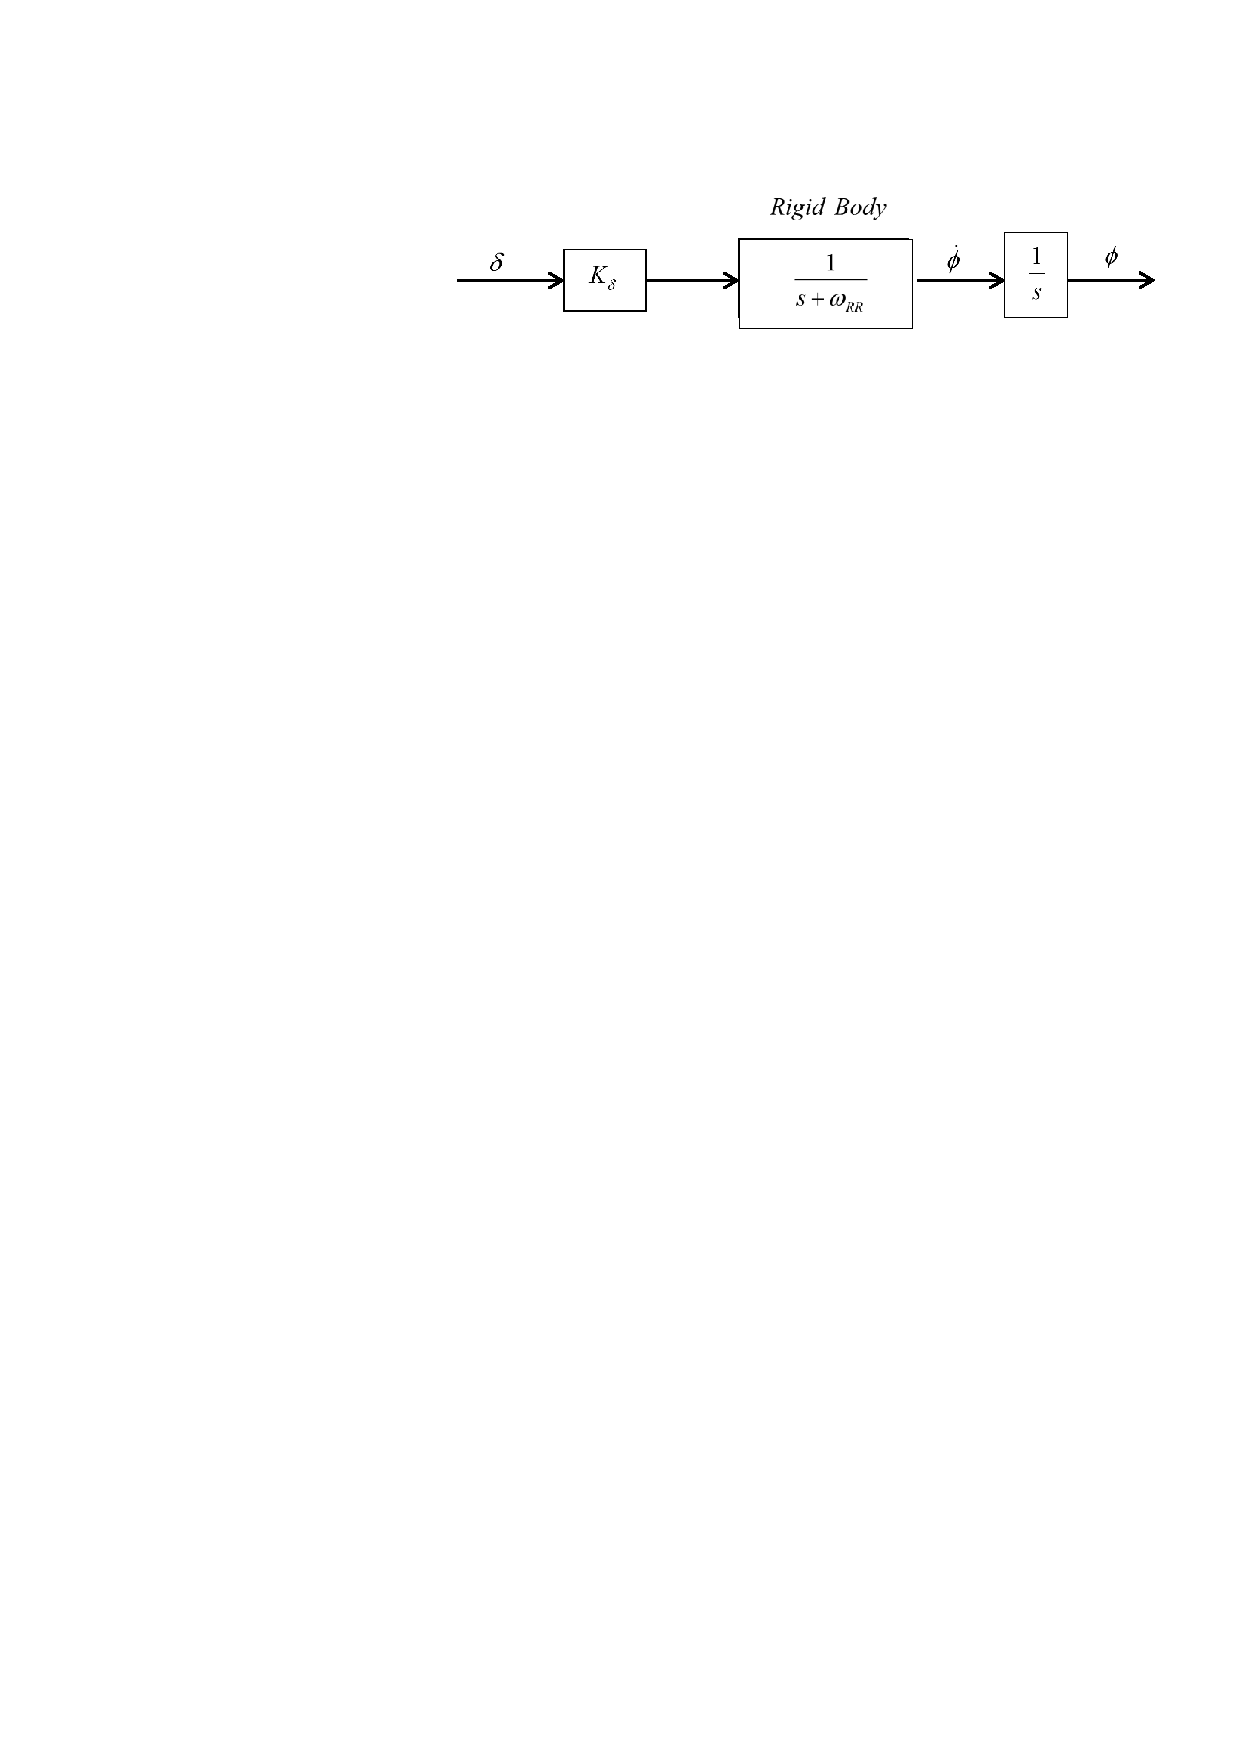
\includegraphics[width=8.4cm]{fig1}    % The printed column width is 8.4 cm.
\caption{Block Diagram Schematic of roll dynamics} 
\label{fig1}
\end{center}
\end{figure}
%-----------------------------------------------------------------------------------------------------------------------------------------------------------------------------------------------------------
\subsection{Design of UDE based control law}
As stated above, for an ideal actuator $\delta = \delta_c$. Now, defining the states $x_1$ and $x_2$ to be $\phi$ and $p$, respectively, the state space representation for (\ref{eq1}) is as follows;
%
\begin{eqnarray}
\dot{x}_1 &=& x_2 \nonumber \\
\dot{x}_2 &=& - \omega_{RR}x_2 + K_{\delta}\delta
\label{eq2}
\end{eqnarray}
%
Taking into account, the uncertainties in $\omega_{RR}$ and $K_{\delta}$ and external disturbance ($d_{ext}$) acting on the system, we can express the actual value of roll rate bandwidth as $\omega_{RR}= \omega_{RR n}+\Delta\omega_{RR}$ and actual fin effectiveness as $K_\delta = K_{\delta n}+\Delta K_{\delta}$, where $K_{\delta n}$ and $\omega_{RR n}$ are the nominal values, with the uncertainties being expressed by $\Delta K_{\delta}$ and $\Delta\omega_{RR}$. The dynamics given in (\ref{eq2}) can thus be re-written as
%
\begin{eqnarray}
\dot{x}_1 &=& x_2 \nonumber \\
\dot{x}_2 &=& -( \omega_{RRn} + \Delta\omega_{RR})x_2 + (K_{\delta n} + \Delta K_{\delta} )\delta + d_{ext}
\label{eq3}
\end{eqnarray}
%
Clubbing the uncertainties and the external disturbance terms in (\ref{eq3}), defining $d = -\Delta\omega_{RR}x_2 + \Delta K_{\delta} \delta + d_{ext}$; the dynamics of the plant are now given by
%
\begin{eqnarray}
\dot{x}_1 &=& x_2 \nonumber \\
\dot{x}_2 &=& - \omega_{RRn}x_2 + K_{\delta n}\delta + d
\label{eq4}
\end{eqnarray}
%
With $\delta$ as the control input ($u$), the control law is proposed as
%
\begin{equation}
u = \frac{1}{K_{\delta n}}\left[u_a + u_d + \nu \right]
\label{eq5}
\end{equation}
%
where $u_a =  \omega_{RRn}x_2$ and $\nu$ is that part of the control law which is responsible for driving the system to the desired dynamics. $\nu$ is defined as;
%
\begin{equation}
\nu = \ddot{\phi}_{ref} - m_1(\dot{\phi} - \dot{\phi}_{ref}) - m_2(\phi - \phi_{ref})
\label{eq6}
\end{equation}
%
where $\phi_{ref}$ is the desired output or the reference value, with $\phi$ being the actual roll angle value. $m_1$ and $m_2$ are feedback gains whose values can be chosen as per the desired characteristics.
With $u_a$ and $\nu$ having been defined, we now need to design $u_d$ to cater to the effects of $d$.
As referred in \cite{zhong2004}, we define $\hat d$ to be the estimate of $d$ and relate the two as follows;
%
\begin{equation}
\hat d = \left( \frac{1}{1 + s\tau}\right)d
\label{eq7}
\end{equation}
%
where $\tau$ is the time constant of the first order filter. $\tau$ must be chosen to have a sufficient bandwidth, such that it nullifies the effect of the lumped disturbance $d$. From (\ref{eq4}), $d$ can be defined as;
%
\begin{equation}
d = \dot{x}_2 + \omega_{RRn}x_2 - K_{\delta n}u
\label{eq8}
\end{equation}
%
Using (\ref{eq7}) and (\ref{eq8}), we express $\hat{d}$ as
%
\begin{equation}
\hat d = \left( \frac{1}{1 + s\tau}\right)\left(\dot{x}_2 + \omega_{RRn}x_2 - K_{\delta n}u\right)
\label{eq9}
\end{equation}
%
Taking $u_d = -\hat d$, after few algebraic manipulations, the closed form expression for $u_d$ from (\ref{eq9}) can be derived as;
%
\begin{equation}
u_d= - \frac{1}{\tau}\left[x_2 - \int \nu dt\right]
\label{eq10}
\end{equation}
%
The final UDE based robust control law using (\ref{eq5}), (\ref{eq6}) and (\ref{eq10}) can be written as
%
\begin{equation}
u =  \frac{1}{K_{\delta n}}\left[\omega_{RRn}x_2  - \frac{1}{\tau}\left[x_2 - \int \nu dt\right]+\nu\right]
\label{eq11}
\end{equation}
%
Since the stability analysis for the UDE based control law for similar systems is available in the literature, it has been omitted.
\subsection{Performance analysis of UDE based controller}
To analyze the performance of the plant with an ideal actuator in accordance with the UDE based control law given in (\ref{eq11}), the simulation parameters for the considered tactical missile were chosen using Table. 1 of \cite{talole2011}. 
%
\begin{table}[h]
\begin{center}
\caption{Performance specifications}\label{tb1}
\begin{tabular}{ccc}
\hline
$\omega_{RR}$ & roll rate bandwidth & 2 rad/s\\ \hline
$K_\delta$ & fin effectiveness & 9000 1/$s^2$\\ \hline
$\omega_A$ & actuator bandwidth & 100 rad/s\\ \hline
$\zeta_A$ & actuator damping & 0.65 \\ \hline
$\phi_{max}$ & maximum desired roll angle & 10 deg\\ \hline
$\dot{\phi}_{max}$ & maximum desired roll rate & 300 deg/s\\ \hline
$d_{ext}$ & external disturbance & 200 rad/$s^2$ \\ \hline
$\delta_{cmax}$ & maximum desired fin deflection & 30 deg \\ \hline
\end{tabular}
\end{center}
\end{table}
%
$\tau$ was chosen to be 0.01. With a desired settling time of 180 ms and damping factor of 0.8, the feedback gains $m_1$ and $m_2$ were evaluated to be 42.45 and 771.13, respectively. Simulations were carried out with $\phi$ having an initial condition of 10 deg.
To ascertain the stabilization capability of control law in (\ref{eq11}) in presence of the external disturbance $d_{ext}$ and an uncertainty in $\omega_{RR}$ simulations were carried out. Taking $\omega_{RR}$ to be -3 rad/s , the simulation results are presented in Fig. 2. The results confirm the satisfactory performance of the proposed control law (\ref{eq11}) with a phase margin of 69 deg. A similar performance was also seen when $\omega_{RR}= +3$ rad/s. 
%---------------------------------figure2-------------------------------------------------------------------------------------------------------

\begin{figure}[h]
\begin{center}
	%\begin{subfigure}
	%\subfigure[Output Response]{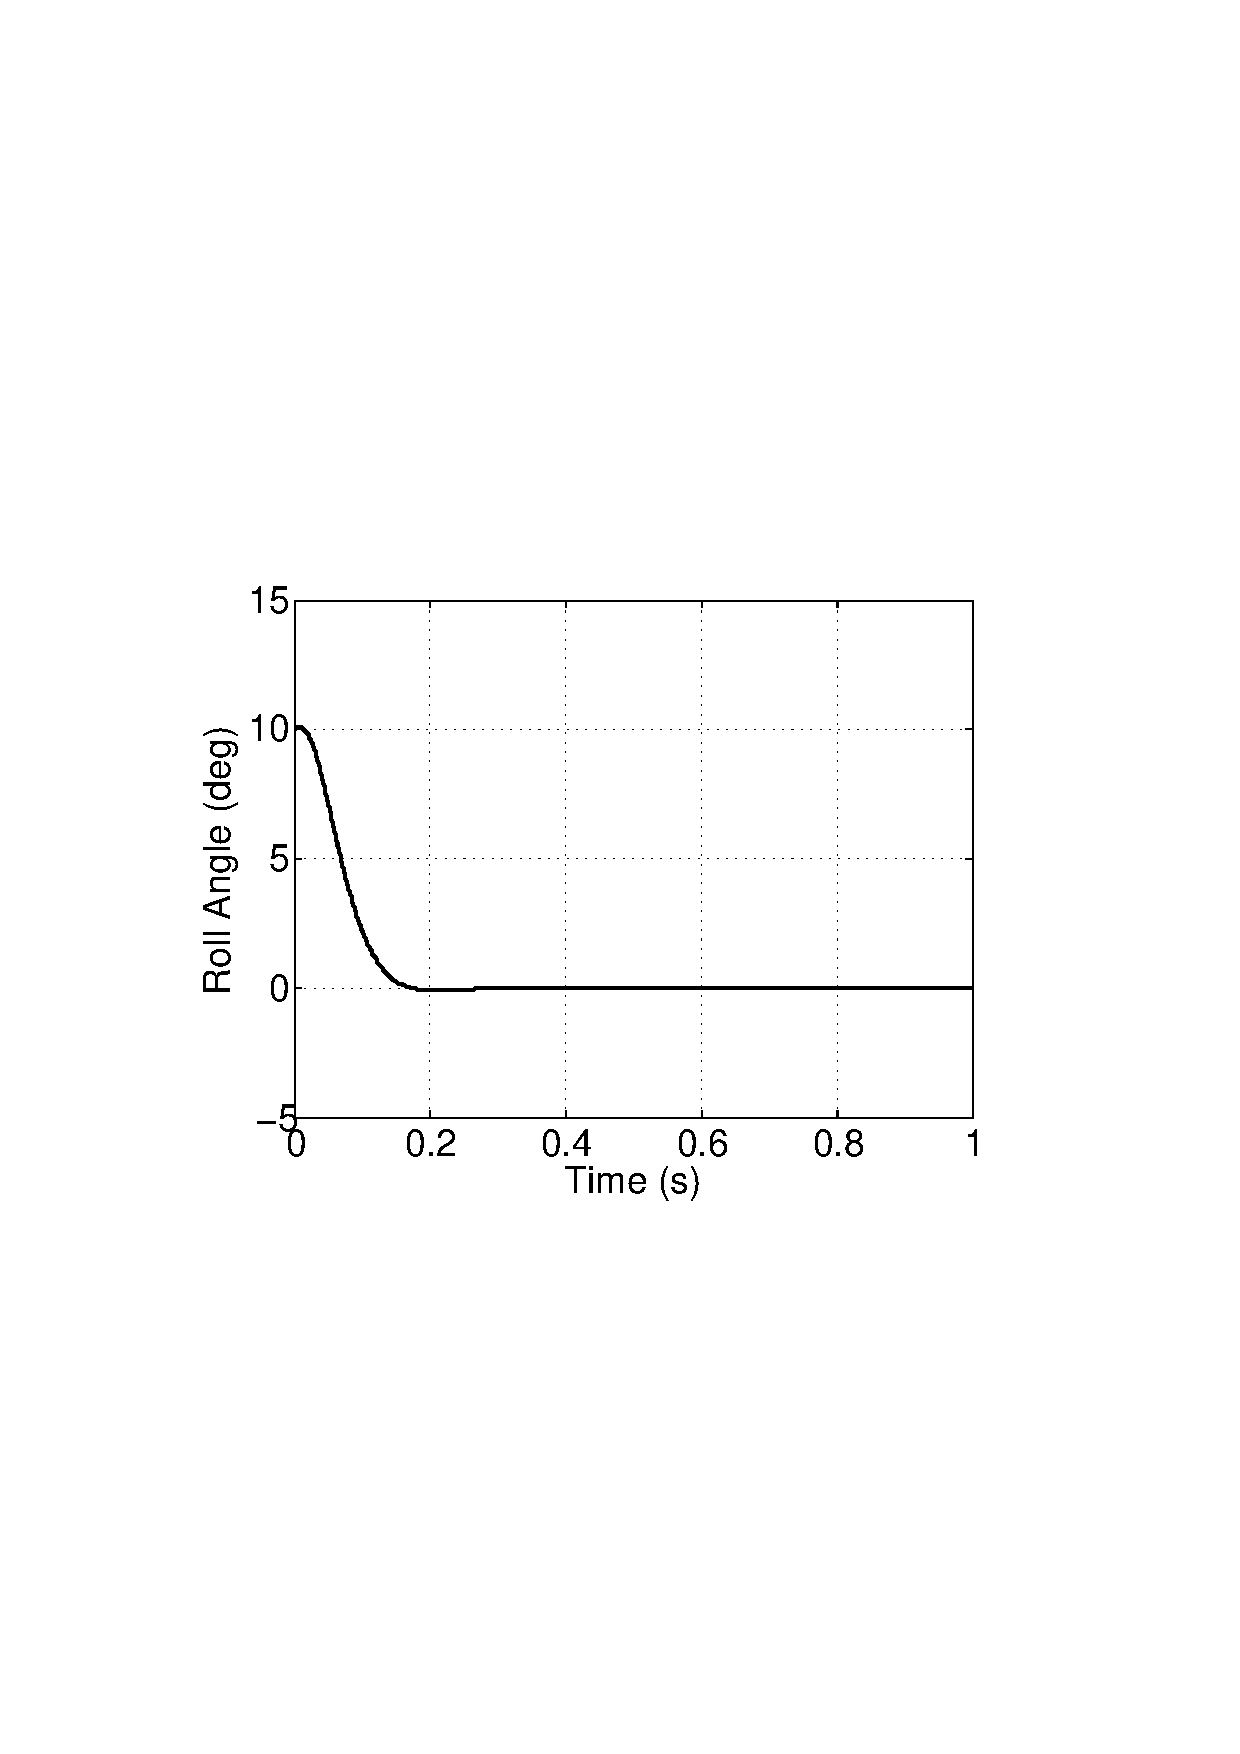
\includegraphics[width=8.4cm]{fig2a}}
	\subfigure[Output Response]{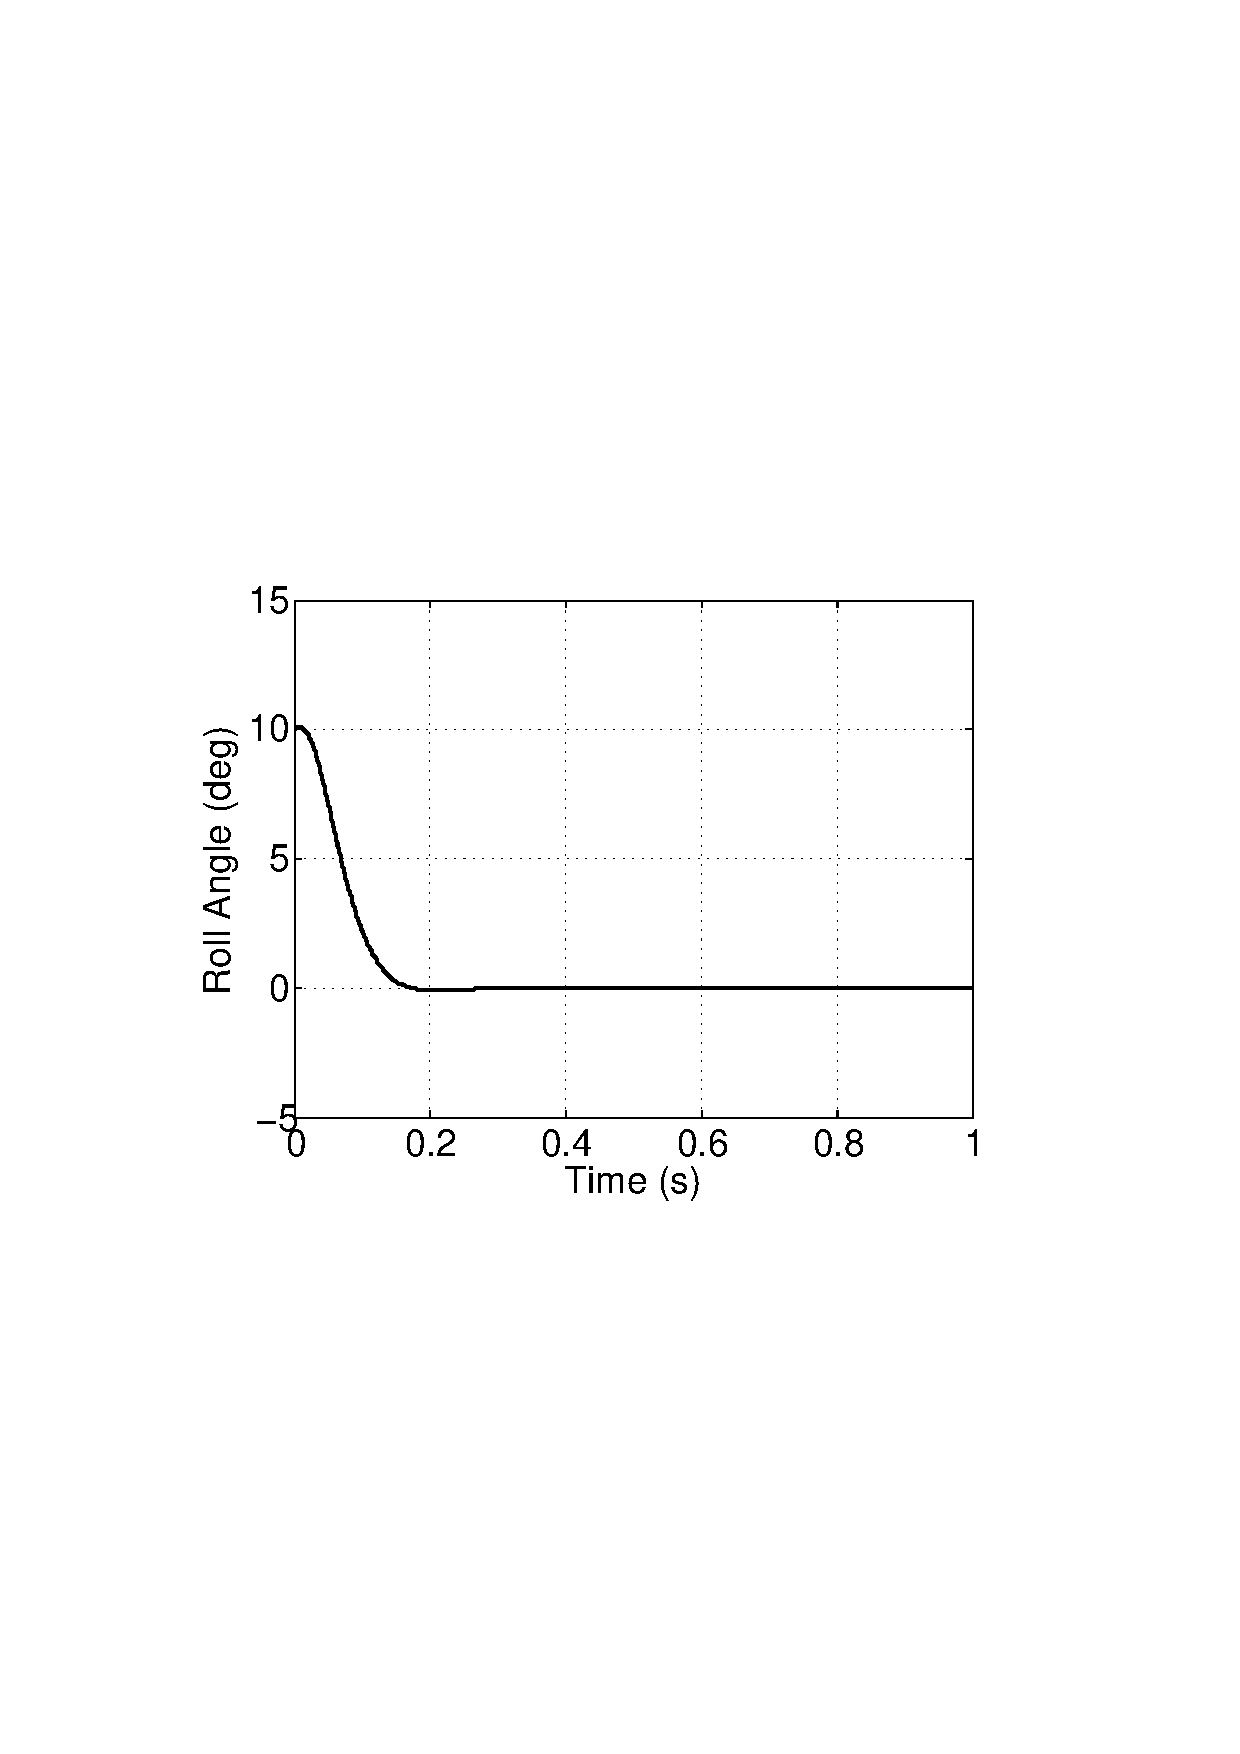
\includegraphics[width=4cm]{fig2a}}
	%\includegraphics[width=8.4cm]{fig3a}    % The printed column width is 8.4 cm.
	%\caption{Output response}
	%\end{subfigure}
%
	%\begin{subfigure}
	\subfigure[Control Effort]{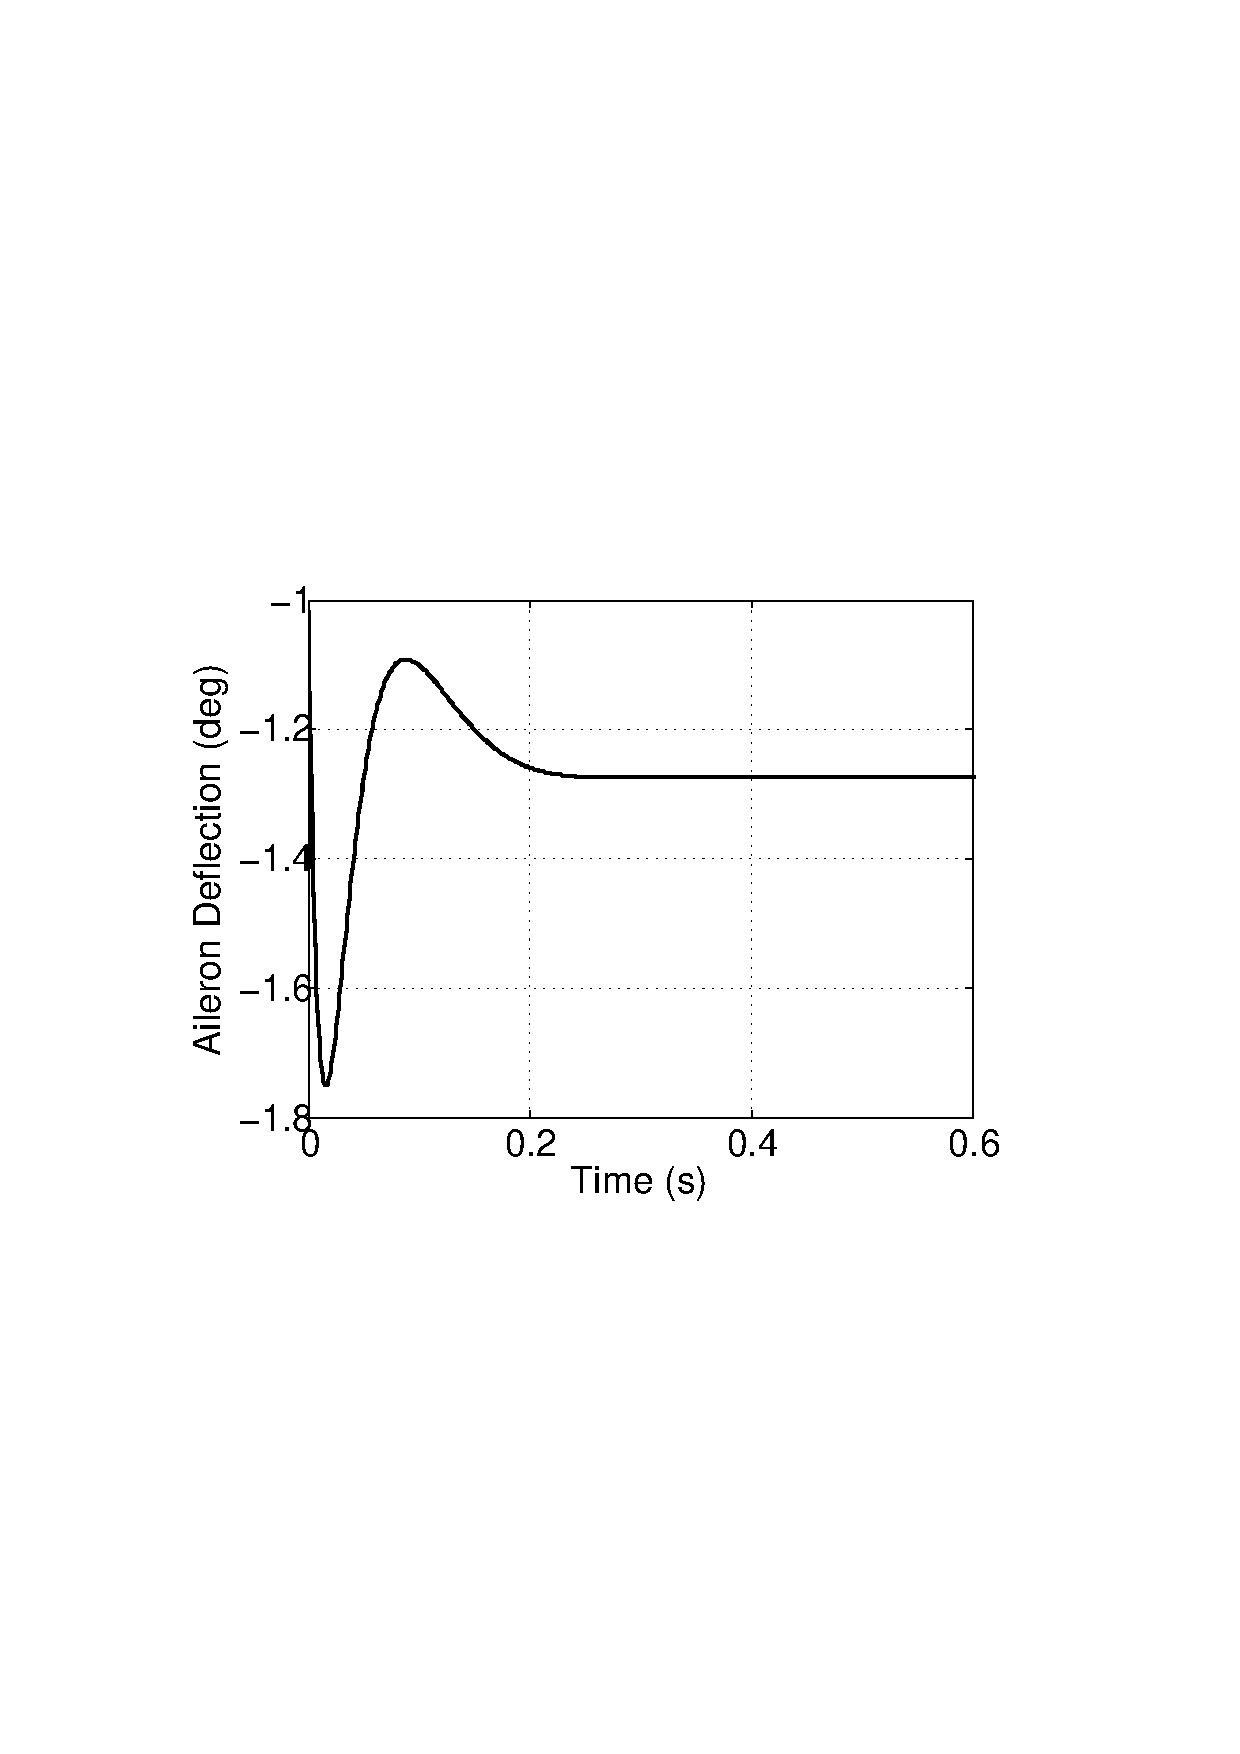
\includegraphics[width=4cm]{fig2b}}
	%\includegraphics[width=8.4cm]{fig3b}    % The printed column width is 8.4 cm.
	%\caption{Control Effort}
	%\end{subfigure}
	\subfigure[Disturbance Estimation]{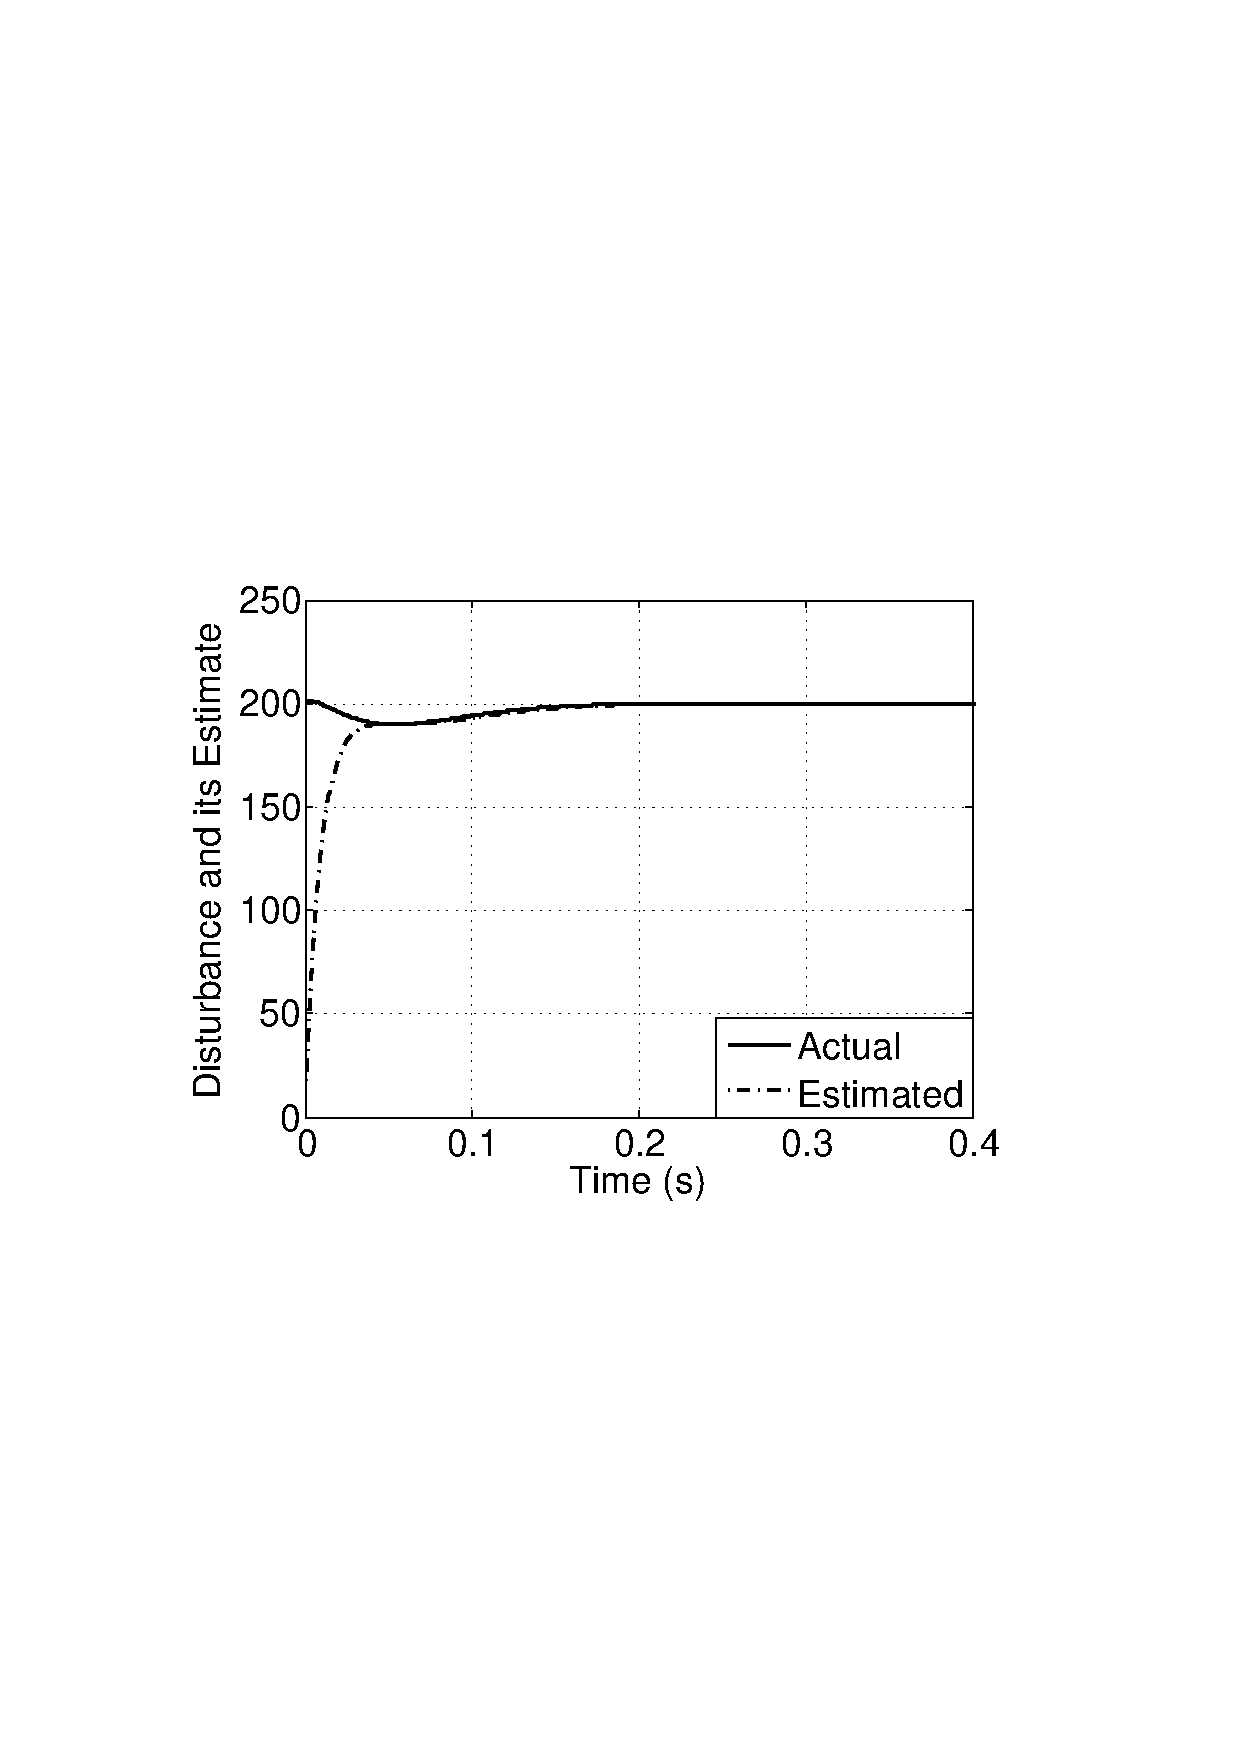
\includegraphics[width=4cm]{fig2c}}
	\caption{Performance of UDE based controller with ideal actuator in presence of disturbances and uncertainties} 
\label{fig2}
\end{center}
\end{figure}
%%--------------------------------------------------------------------------------------------------------
UDE based control law thus exhibits a satisfactory performance in the presence of external disturbances as well as uncertainties, assuming ideal actuator.
%%----------------------------------------------------------------------------------------------------------------------------------------------------------------------------------------------------------------------------------------------------------------------------------------------------------------------------------------------------------------Section 2 -------------------------------------------------------------------------------------------------------------------------
\subsection{Performance of UDE based controller with second order actuator in the loop}
An actuator modeled as a second order transfer function, as referred in \cite{talole2011}, of the form ${{\delta (s)}\over{\delta_c(s)}} = {{\omega^2_A}\over{s^2 + 2\zeta_A \omega_A s + \omega^2_A}}$ is introduced in the plant, as illustrated in Fig. 3. Here $\omega_A$ is the actuator bandwidth and $\zeta_A$ is the actuator damping ratio.
%--------------------------------------------------------------------------------- To insert Fig. 4--------------------------------------------
% 
\begin{figure}[h]
\begin{center}
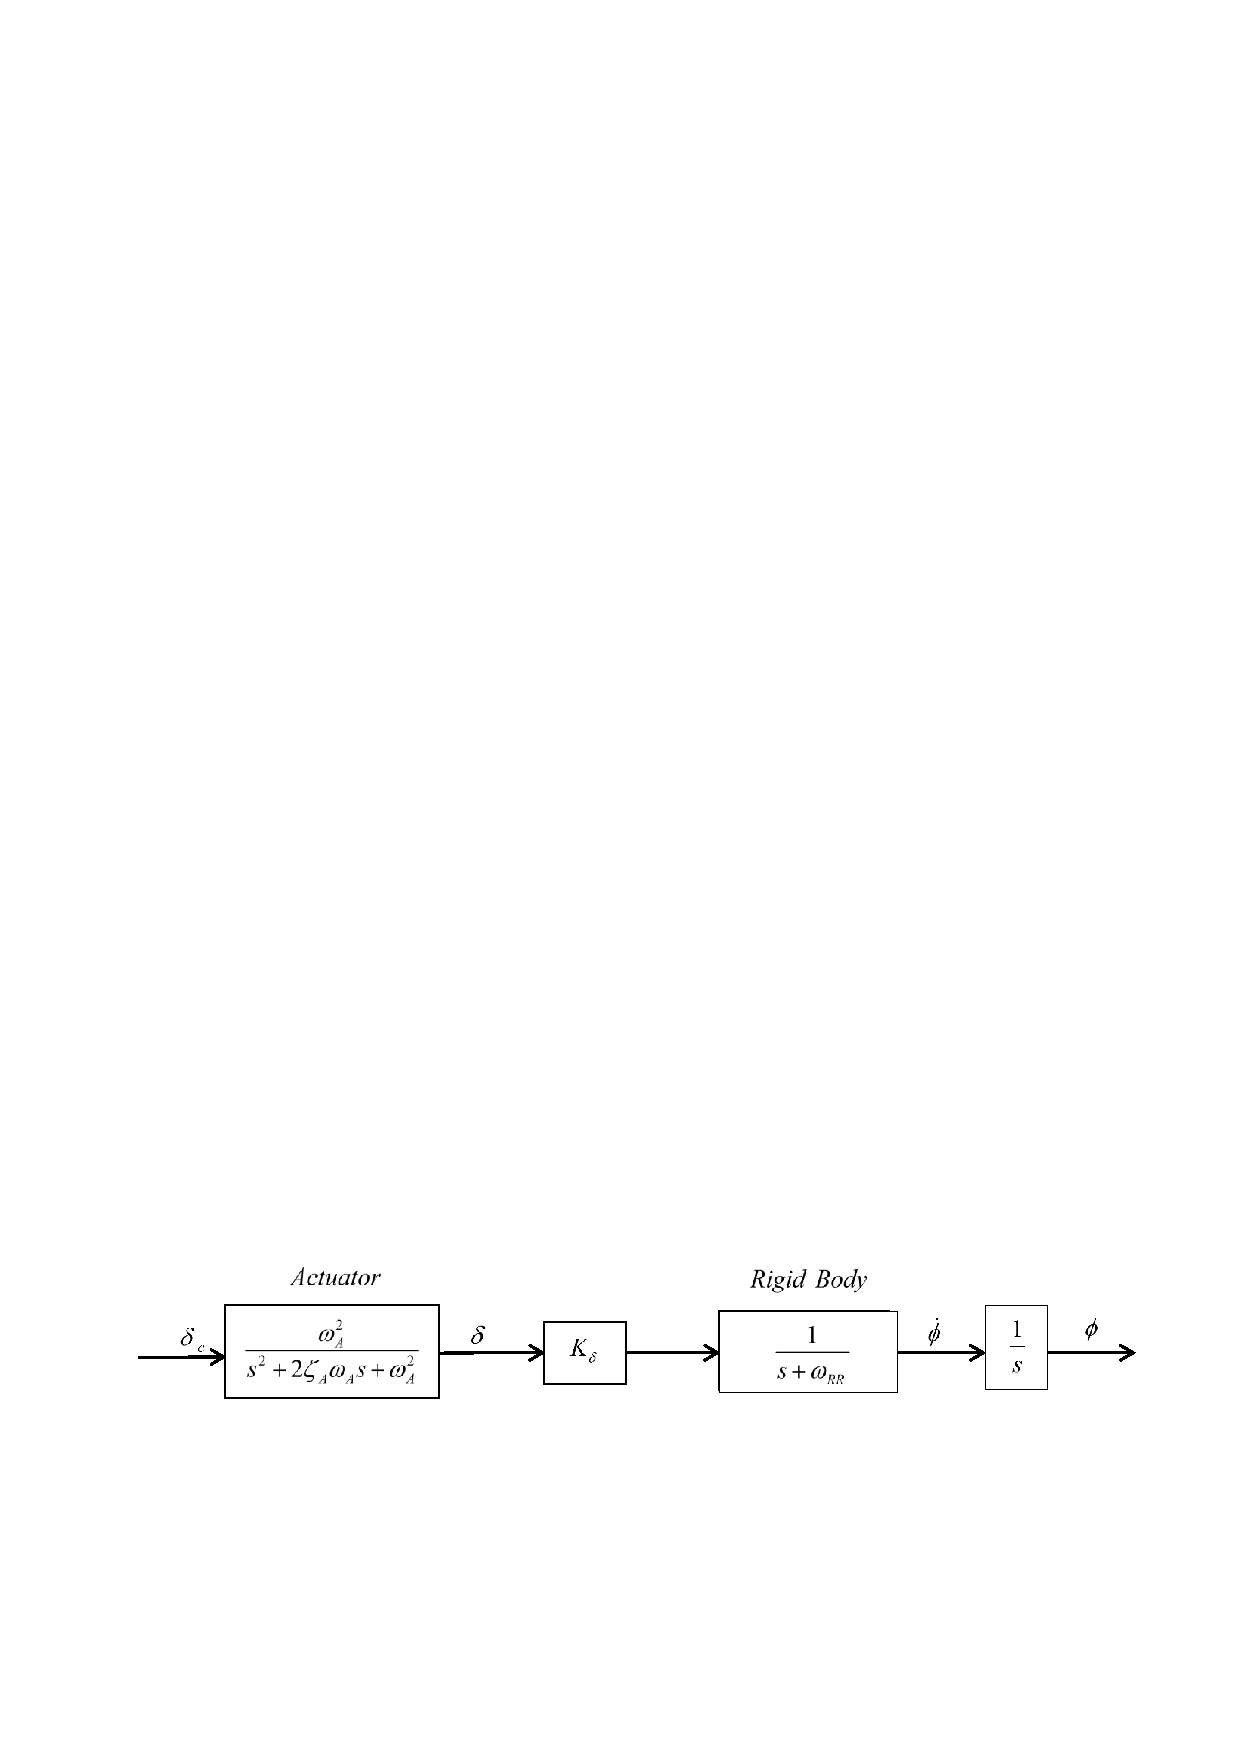
\includegraphics[width=8.4cm]{fig4}    % The printed column width is 8.4 cm.
\caption{Schematic of roll dynamics with second order actuator} 
\label{fig3}
\end{center}
\end{figure}
Simulations were carried out with the parameter values as specified in Table. 1, using the control law defined in (\ref{eq11}), with $\tau$ as 0.01. In this case only disturbance of $d_{ext}$ has been considered. Since actuator dynamics included here were unaccounted for in the design of control law in (\ref{eq11}), the performance of the system does not remain the same as in previous case, as can be seen in Fig. 4. 

%%-------------------------------------------------------------------------------Figure5-------------------------------------------------------------------
%
\begin{figure}[h]
\begin{center}
	%\begin{subfigure}
	%\subfigure[Output Response]{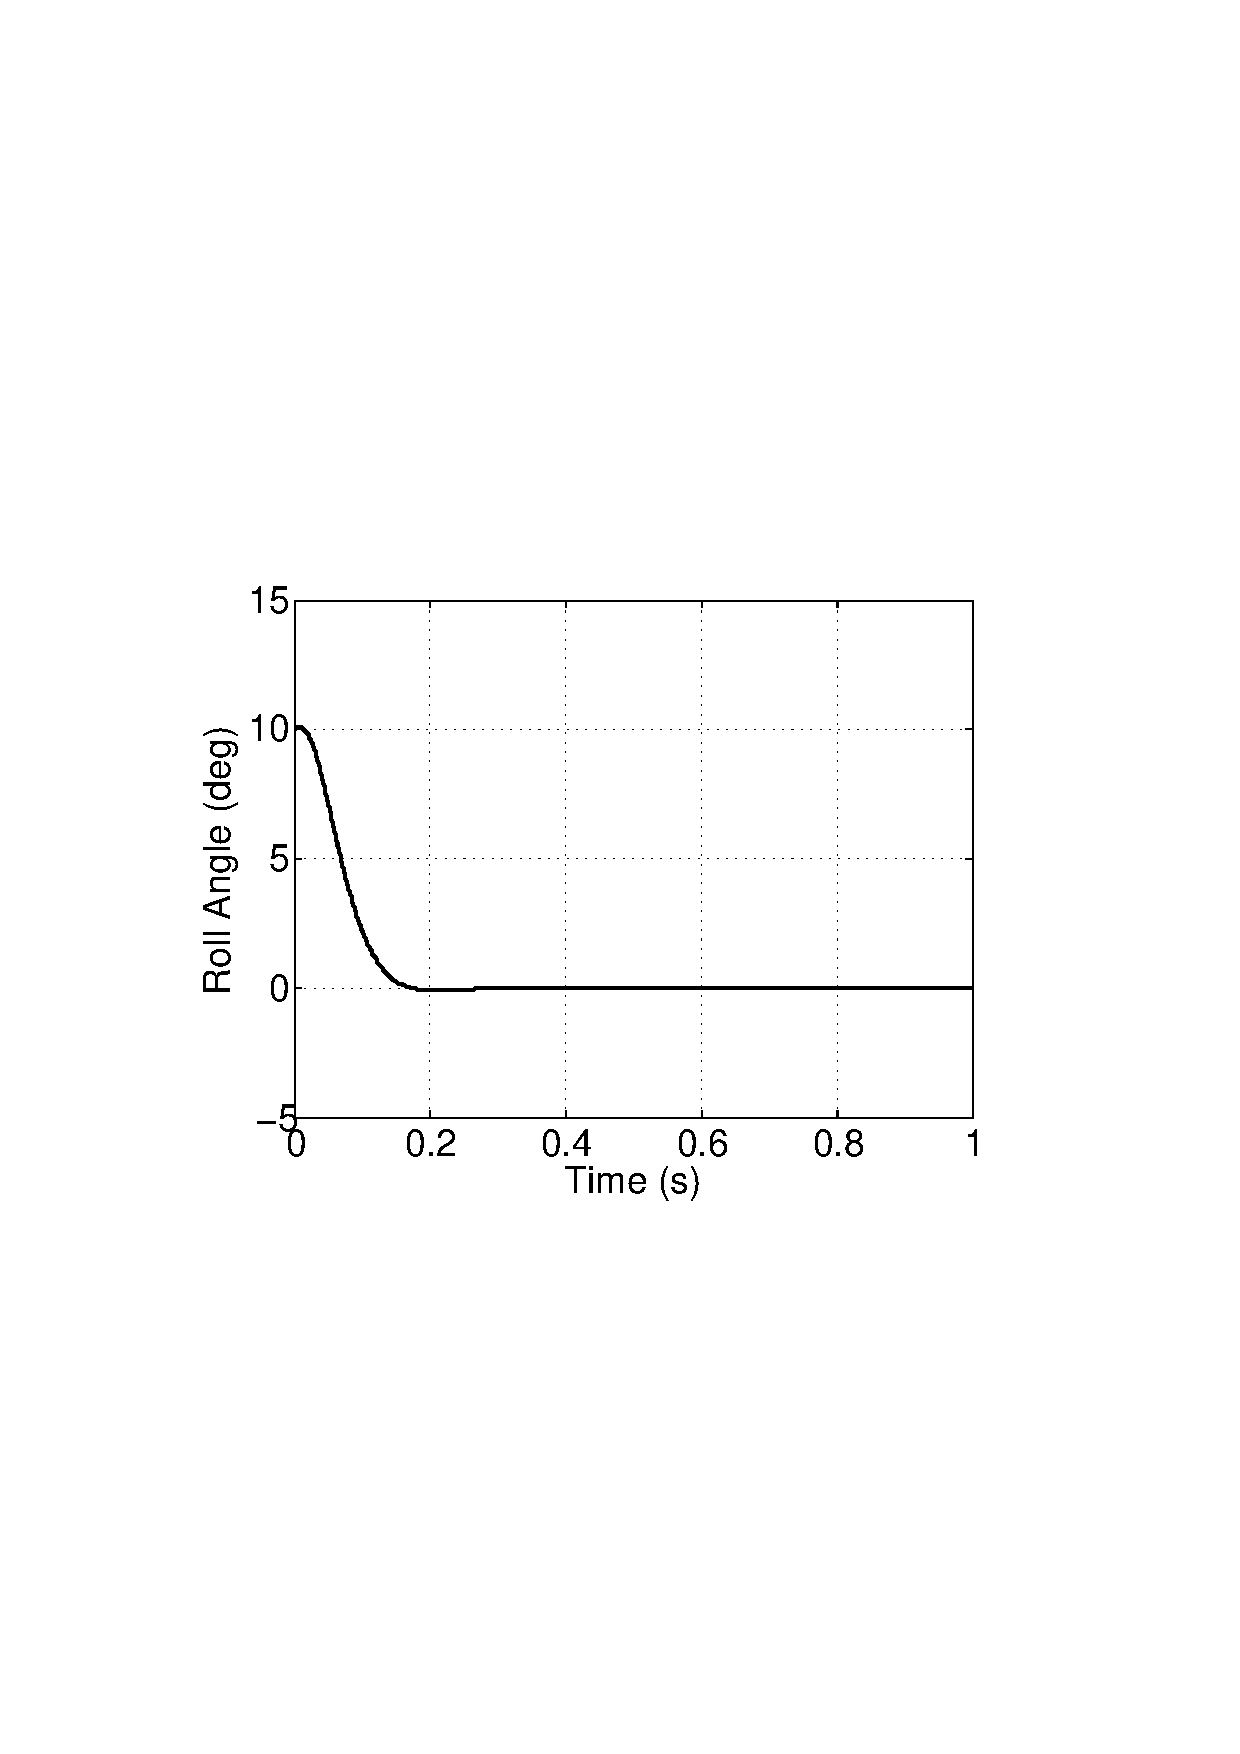
\includegraphics[width=8.4cm]{fig2a}}
	\subfigure[Output Response]{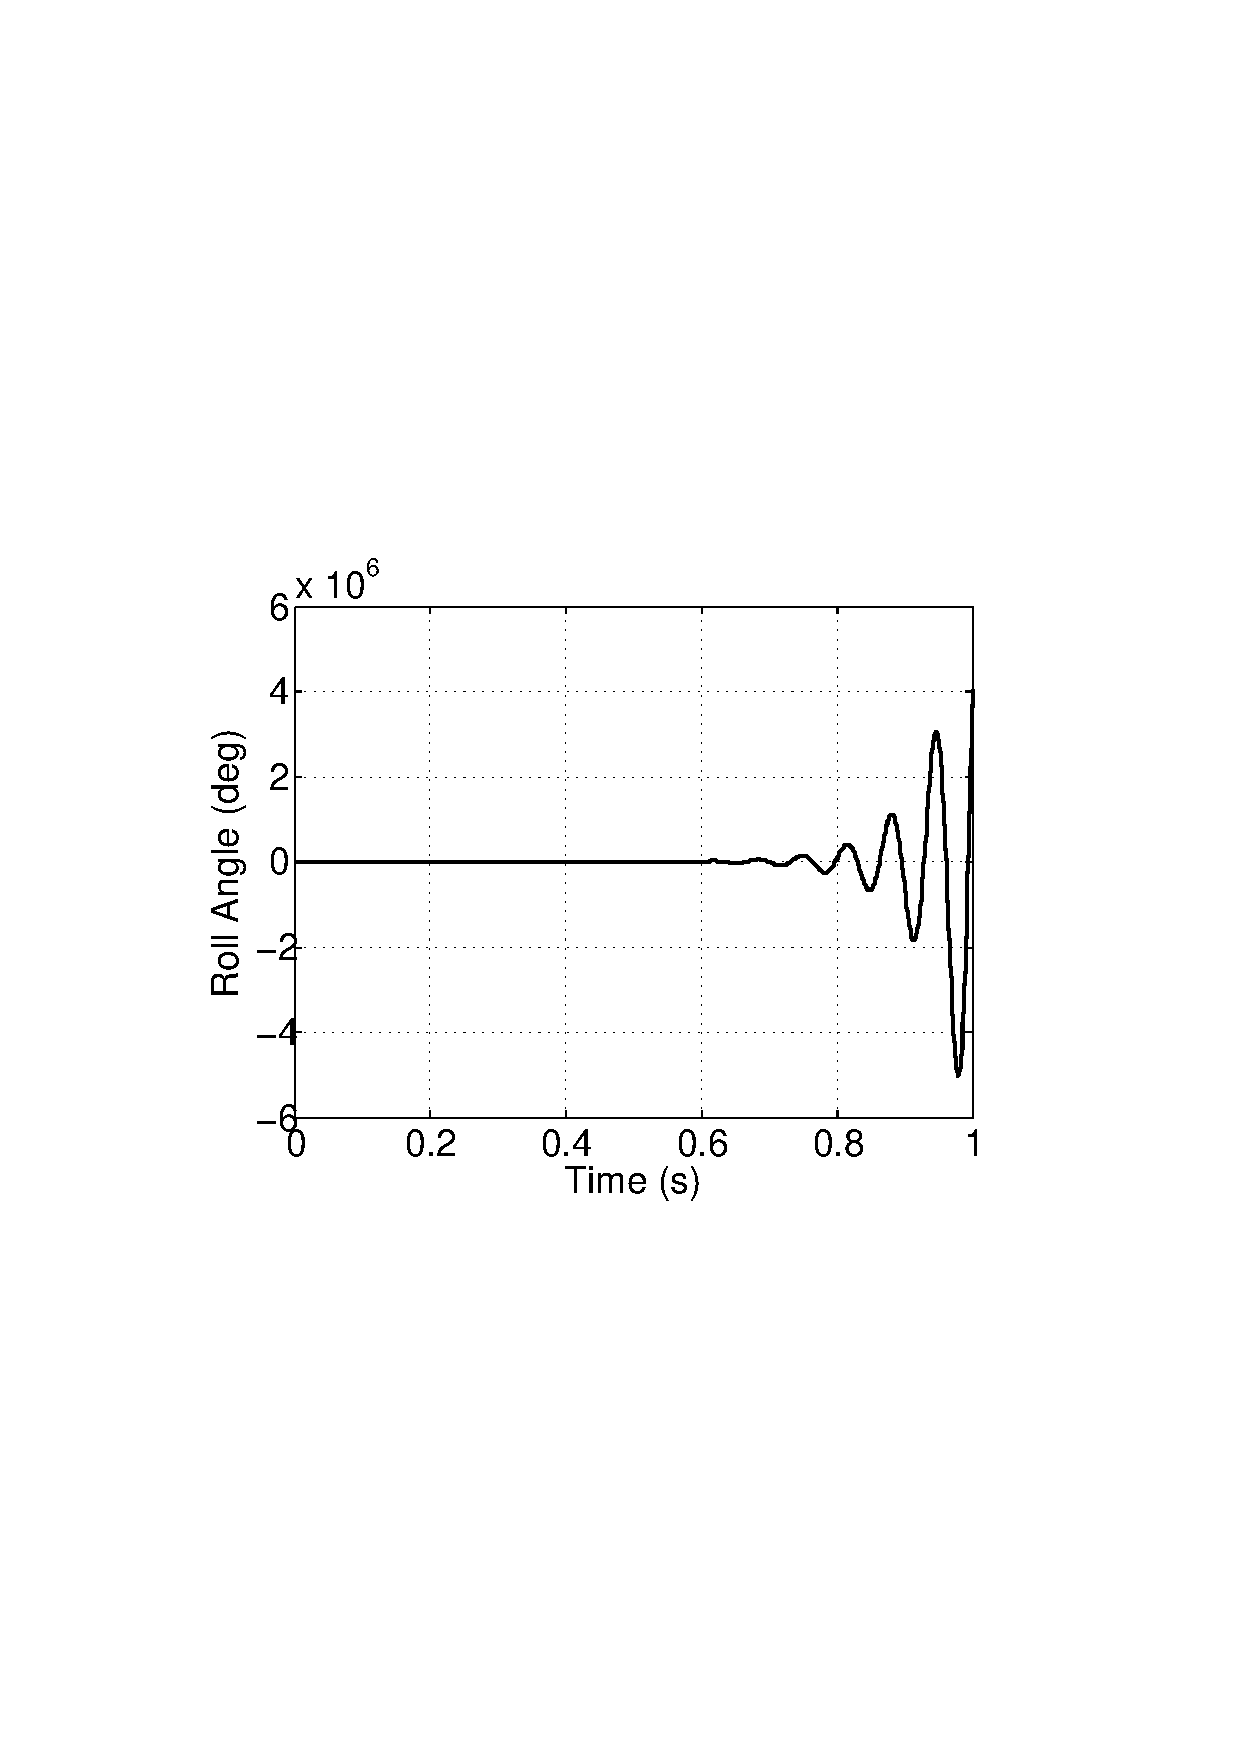
\includegraphics[width=4cm]{fig5a}}
	%\includegraphics[width=8.4cm]{fig3a}    % The printed column width is 8.4 cm.
	%\caption{Output response}
	%\end{subfigure}
%
	%\begin{subfigure}
	\subfigure[Control Effort]{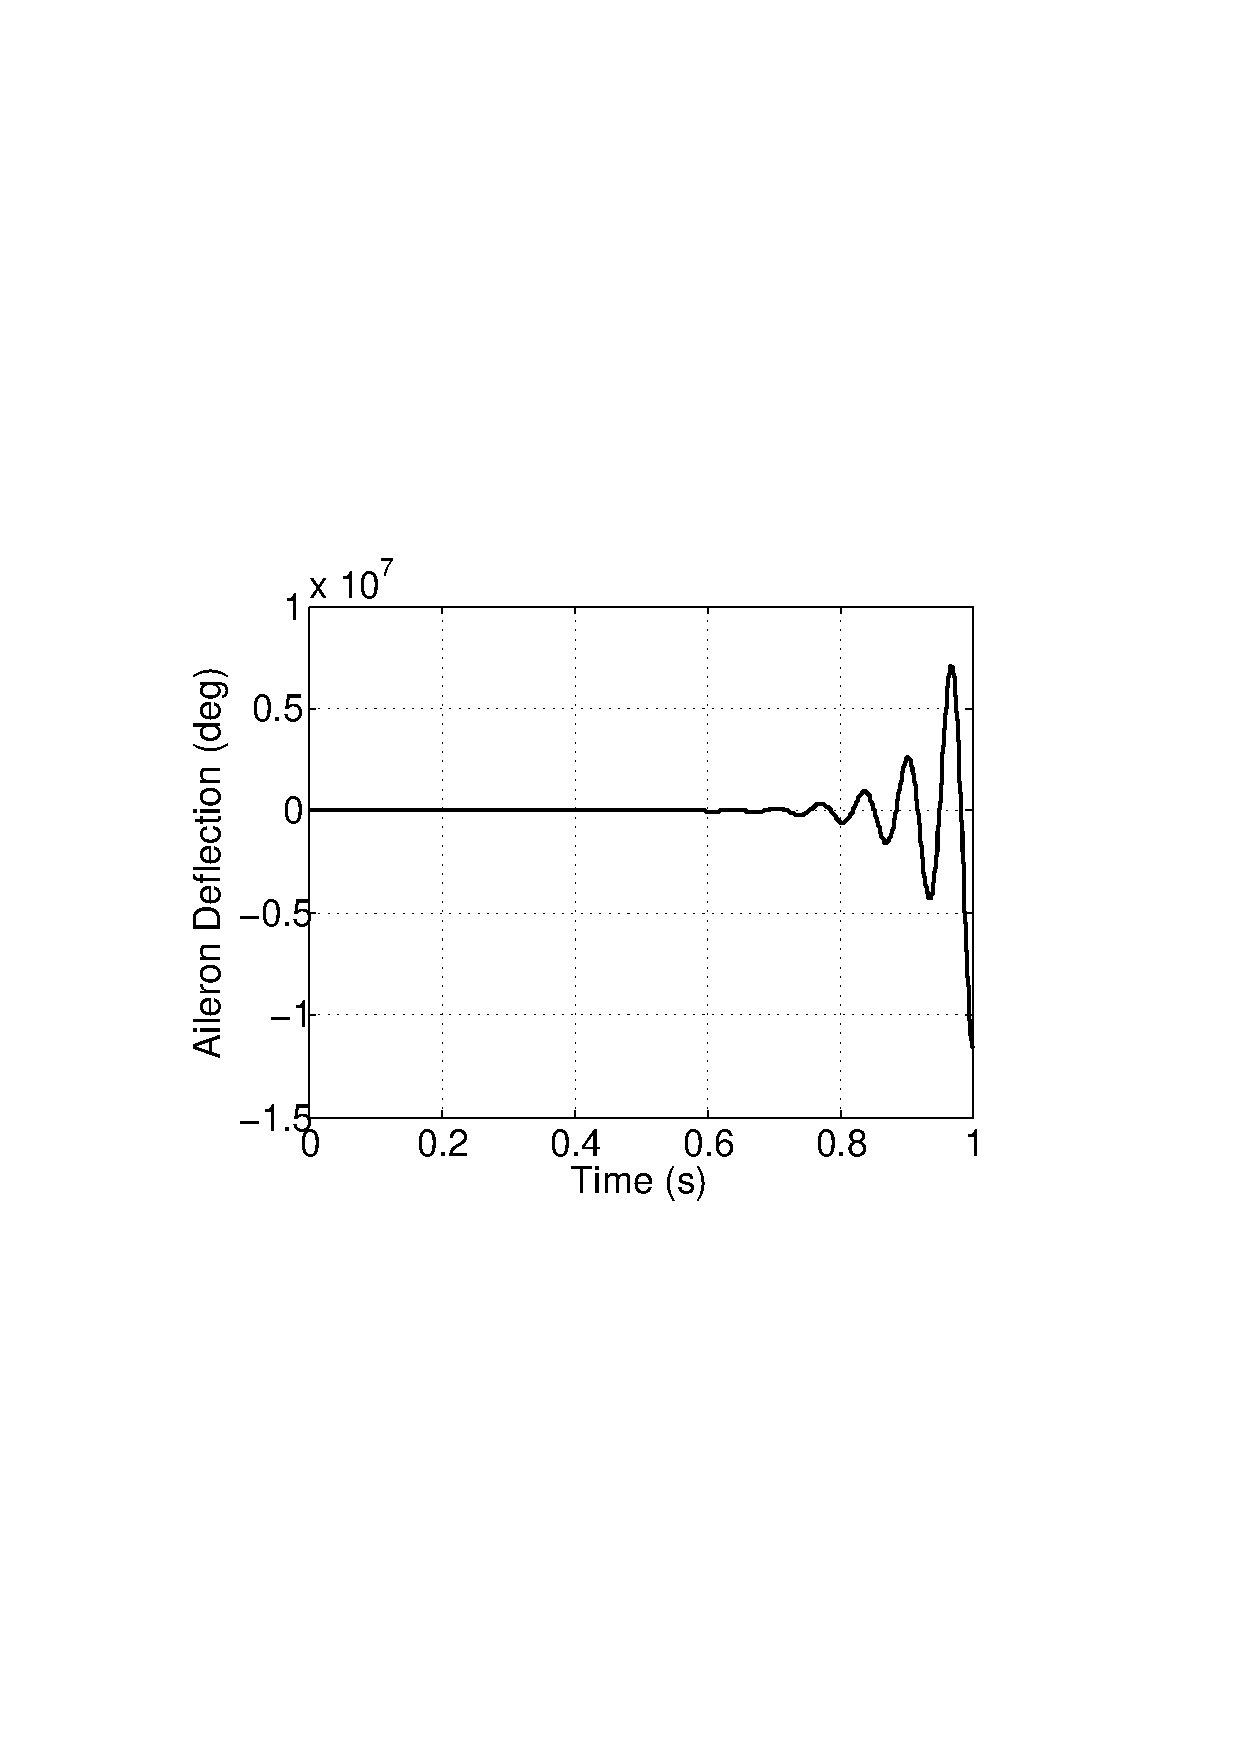
\includegraphics[width=4cm]{fig5b}}
	%\includegraphics[width=8.4cm]{fig3b}    % The printed column width is 8.4 cm.
	%\caption{Control Effort}
	%\end{subfigure}
	\subfigure[Disturbance Estimation]{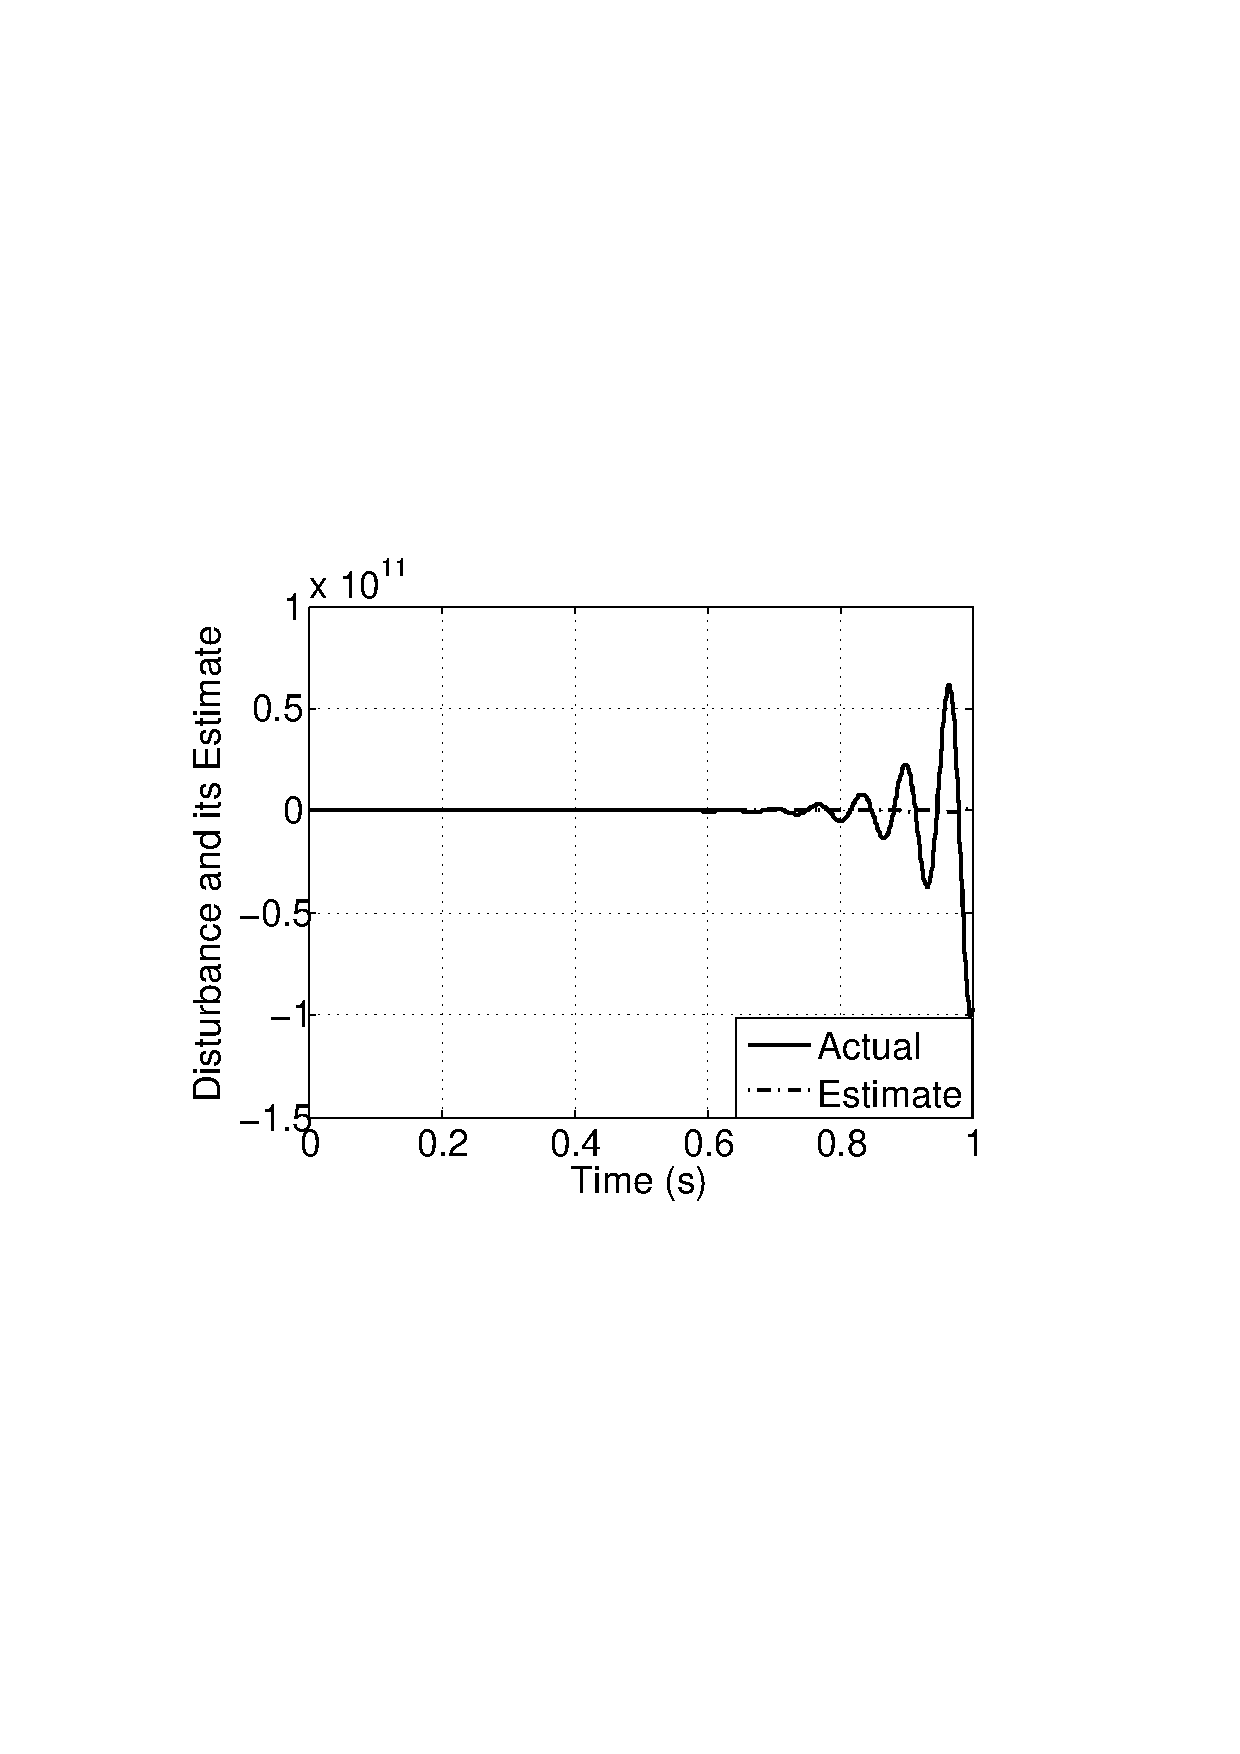
\includegraphics[width=4cm]{fig5c}}
	\caption{Performance of system with second order actuator}  
\label{fig4}
\end{center}
\end{figure}
%%--------------------------------------------------------------------------------------------------------
%%----------------------------------------------------------------------------------------------------------------------------------------------------------------------------------------------------------------------
%%-------------------------------------------------------------------------------------------------------------------------------------------------------------------------------
\section{Actuator compensated UDE based control law}

It has been noted that the addition of a second order actuator to the plant has rendered the system unstable. The reason for this instability is an additional lag introduced by the actuator. Hence there is a need to compensate the effects of the actuator by proper tuning the UDE based robust control law or design a compensator for the actuator. The attempts thus made are explained in the subsequent discussion.

\subsection{Method 1: Tuning of $\tau$}
As inferred from Fig. 3, the relation between $\delta$ and $\delta_c$ is as follows
%
\begin{equation}
\delta = \delta_c - \left[{{1}\over{\omega^2_A}}\left( \ddot \delta + 2\zeta_A \omega_A \dot \delta\right)\right]
\label{eq12}
\end{equation}
%
As $\delta_c$ is the only control available for design purposes, the plant as expressed in (\ref{eq4}) can be represented as
%
\begin{eqnarray}
\dot{x}_1 &=& x_2 \nonumber \\
\dot{x}_2 &=& - \omega_{RRn}x_2 + K_{\delta n}\left[\delta_c - {{1}\over{\omega^2_A}}\left( \ddot \delta + 2\zeta_A \omega_A \dot \delta\right)\right] \nonumber \\
&& + d
\label{eq13}
\end{eqnarray}
%%
Since ${{-K_\delta n}\over{\omega^2_A}}\left( \ddot \delta + 2\zeta_A \omega_A \dot \delta\right)$ is unknown, it can be treated as an unknown disturbance and clubbed with $d$ and denoted as $d_1$. 
\begin{equation}
d_1 = {{-K_\delta n}\over{\omega^2_A}}\left( \ddot \delta + 2\zeta_A \omega_A \dot \delta\right) + d
\label{eq14}
\end{equation}
%%
The resultant plant dynamics thus become;
%
\begin{eqnarray}
\dot{x}_1 &=& x_2 \nonumber \\
\dot{x}_2 &=& - \omega_{RRn}x_2 + K_{\delta n}\delta_c + d_1
\label{eq15}
\end{eqnarray}
%

For the system (\ref{eq15}), the control law in (\ref{eq5}) remains the same, with $u_a =  \omega_{RRn}x_2$, $\nu = \ddot{\phi}_{ref} - m_1(\dot{\phi} - \dot{\phi}_{ref}) - m_2(\phi - \phi_{ref})$ and $u_d= - \frac{1}{\tau}\left[x_2 - \int \nu dt\right]$. The feedback gains $m_1$ and $m_2$ also remain the same.
It is to be noted that the plant continues to be driven through $\delta$, in keeping with the physical structure of the system.
Unlike previous discussions, the control term $u_d$ now caters to the additional disturbance term  ${{-K_\delta n}\over{\omega^2_A}}\left( \ddot \delta + 2\zeta_A \omega_A \dot \delta\right)$ in addition to $d$. This calls for careful choice of $\tau$ to take care of $d_1$.
%%------------------------------------------------------------------------------------------------------------------------------------------------------
\subsubsection{Performance analysis of UDE based controller with actuator compensation using Method 1}
Simulations were carried out with the data given in Table. 1, along with an external disturbance $d_{ext}$. The time constant $\tau$ when chosen to be 0.01, rendered the system unstable. Hence it was varied to achieve the desired performance. It was observed that as the value of $\tau$ increases from 0.01 till 0.025, the system remained unstable, as in Fig. 4. On further increasing the value of $\tau$, the system gradually began to stabilize. The value of $\tau$ which gave the best possible performance was $\tau = 0.04$, the results of which can be seen in Fig. 5.
%%-----------------------------------------------------Figure6--------------------------------------------------------------------%%
\begin{figure}[h]
\begin{center}
	%\begin{subfigure}
	\subfigure[Output Response]{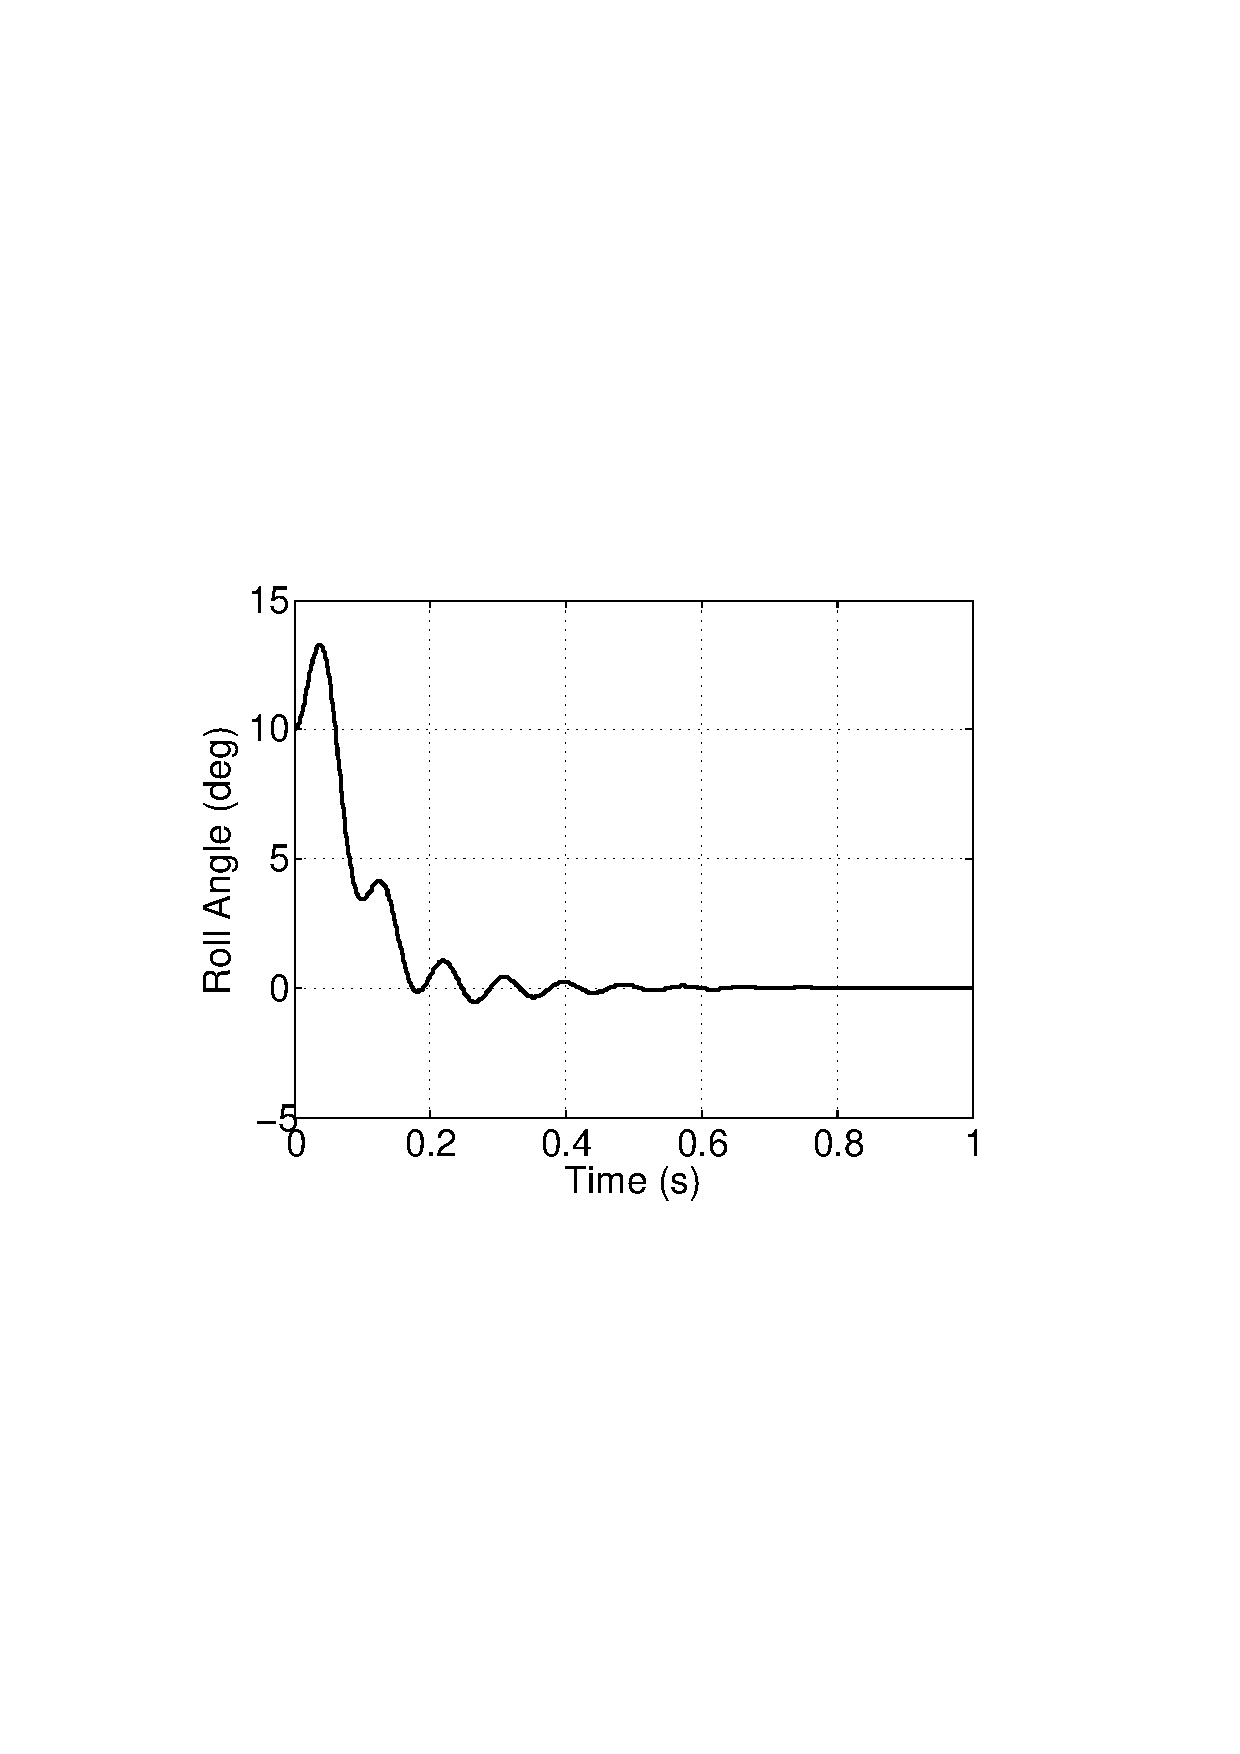
\includegraphics[width=4cm]{fig6a}}
	%\subfigure[Output Response]{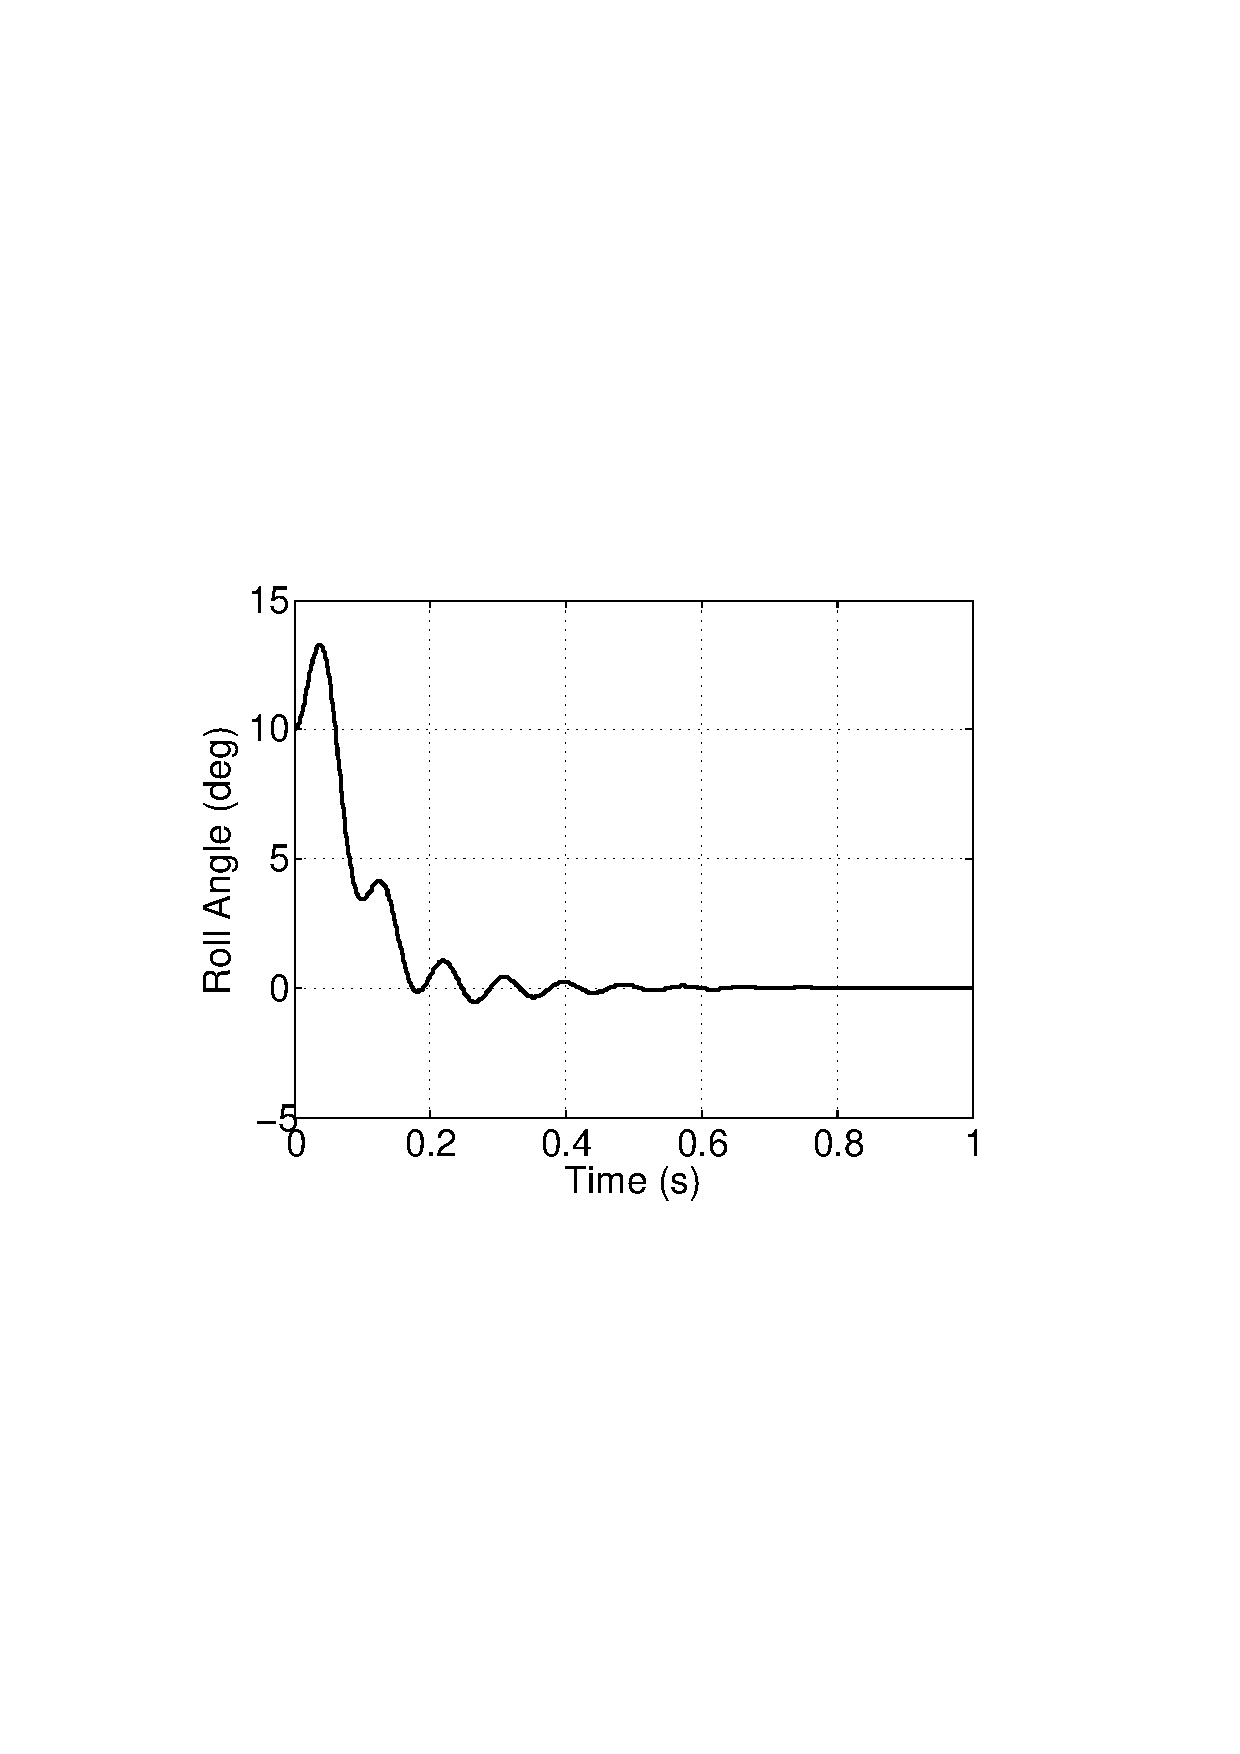
\includegraphics[width=4cm]{fig6a}}
	%%\includegraphics[width=8.4cm]{fig3a}    % The printed column width is 8.4 cm.
	%%\caption{Output response}
	%%\end{subfigure}
%%
	%%\begin{subfigure}
	\subfigure[Control Effort]{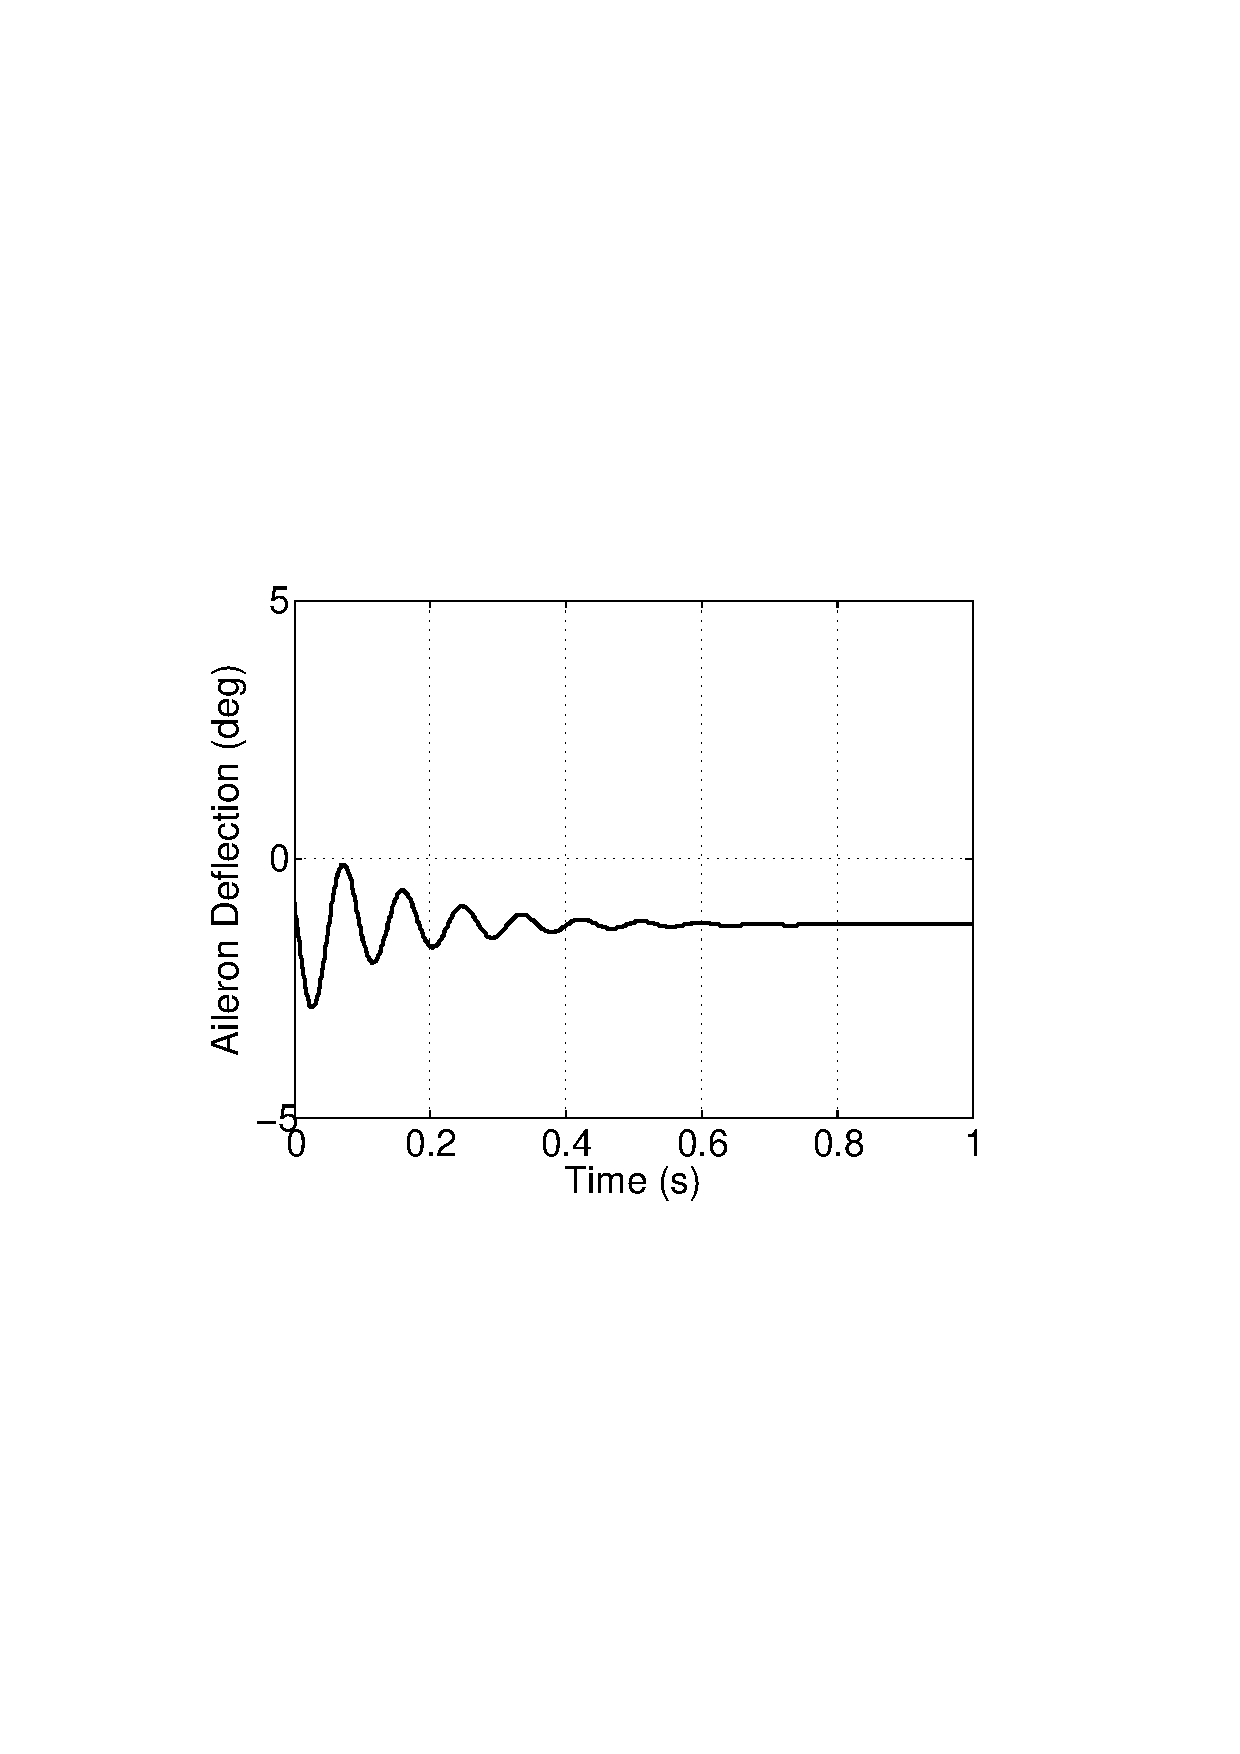
\includegraphics[width=4cm]{fig6b}}
	%%\includegraphics[width=8.4cm]{fig3b}    % The printed column width is 8.4 cm.
	%%\caption{Control Effort}
	%%\end{subfigure}
	\subfigure[Disturbance Estimation]{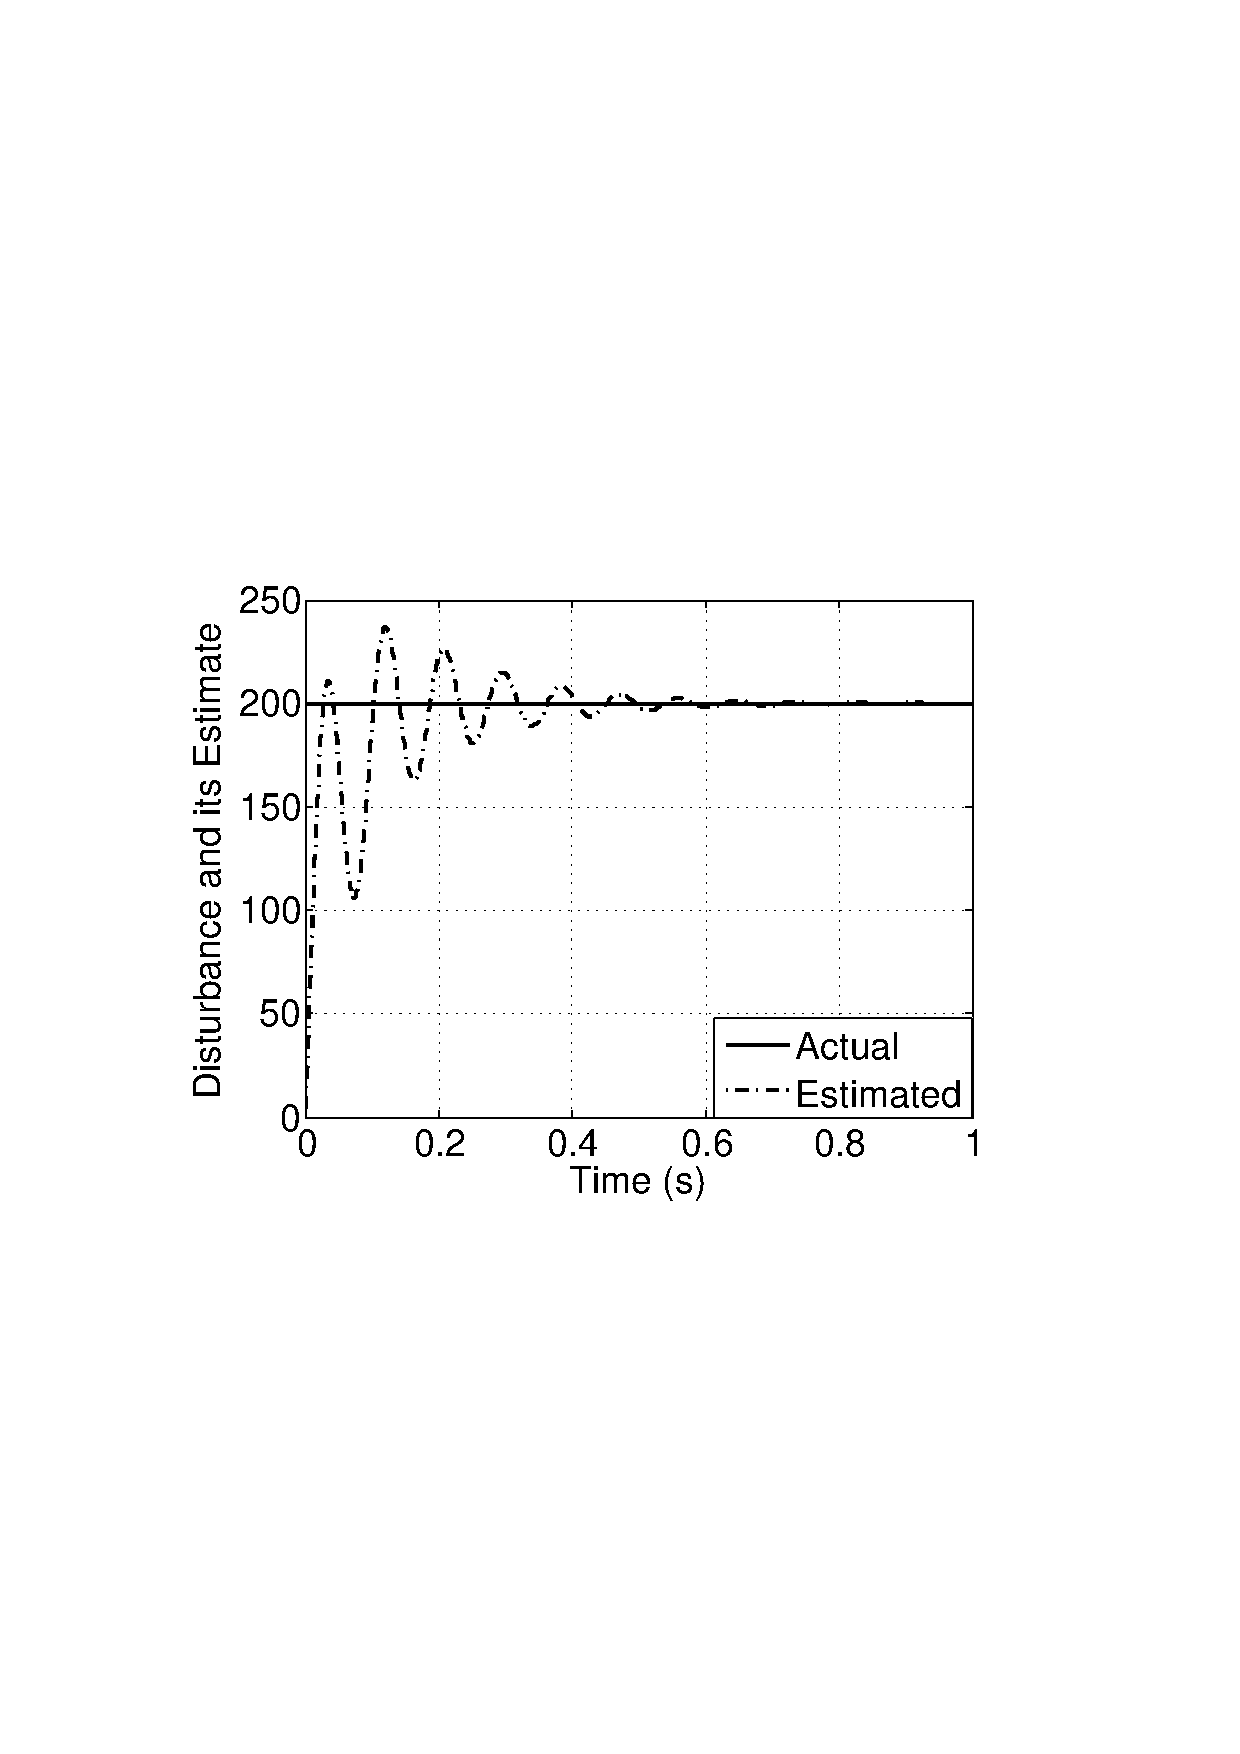
\includegraphics[width=4cm]{fig6c}}
	\caption{Performance with Method 1} 
\label{fig5}
\end{center}
\end{figure}

%%----------------------------------------------------------------------------------------------------------------------------------------------------------------------
From Fig. 5a, it can be seen that the roll angle does not show a smooth descent to equilibrium. An overshoot from its initial condition of 10 deg was also observed, which was dependent on the magnitude of the disturbance. Disturbance estimation was found to be satisfactory after 500 ms and the control effort was found to be oscillatory, though within acceptable limits.
It can thus be inferred, that tuning of $\tau$ did help the system in attaining stability but not to the desired extent, as was shown in Fig. 2.
  
%%--------------------------------------------------------------------------------------------------------------------------------
\subsection{Method 2: Using Compensator Form 1}
Due to the presence of a second order actuator in the loop, there is a lag between $\delta$ and $\delta_c$. The primary aim is to ensure that $\delta$ tracks $\delta_c$ in a sufficiently small time interval which would require a compensator, as inferred from \cite{chwa2004}. In this direction, an attempt has been made to design a compensator, cascaded with the actuator, to reduce the delay. The schematic is shown in Fig. 6
%- ---------------------------------------------------Figure7----------------------------------------------------------------------
\begin{figure}[h]
\begin{center}
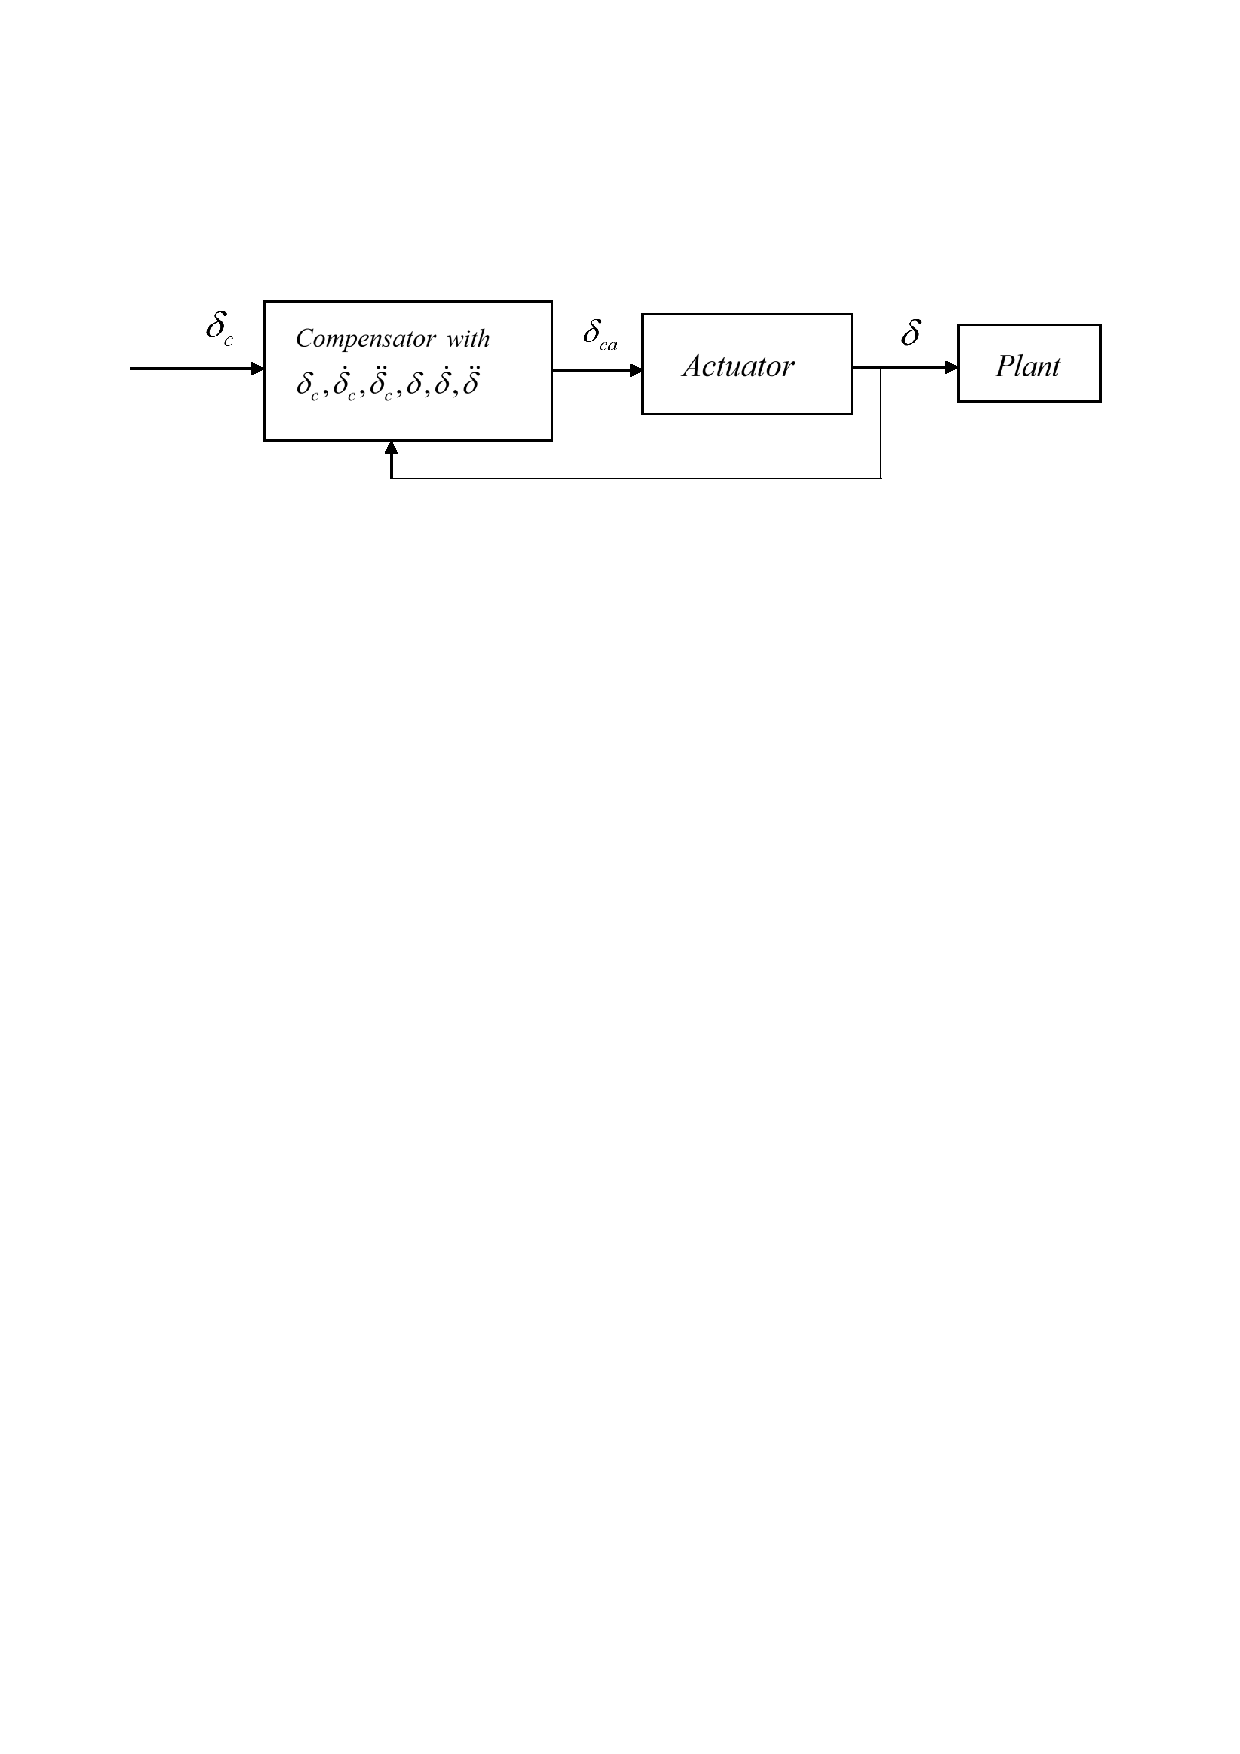
\includegraphics[width=8.4cm]{fig7}    % The printed column width is 8.4 cm.
\caption{Block Diagram Schematic for Method 2} 
\label{fig6}
\end{center}
\end{figure}
%---------------------------------------------------------------------------------------------------------------------------------
The transfer function of the actuator, as given in Fig. 3 can be written as;
%
\begin{equation}
\ddot{\delta}=-2\zeta_A\omega_A\dot{\delta}-\omega_A^2\delta+\omega_A^2\delta_c
\label{eq16}
\end{equation}
%
Unlike the previous approach where the tuning of $\tau$ was done in the control input $u$ or $\delta_c$, here $\delta_c$ derived in (\ref{eq11}), is taken as a reference signal which $\delta$ is required to track before it is fed to the plant, as depicted in Fig. 6. 
Denoting $\delta_{ca}$ to be the output of the compensator, (\ref{eq16}) can be re-written as;
%
\begin{equation}
\ddot{\delta}=-2\zeta_A\omega_A\dot{\delta}-\omega_A^2\delta+\omega_A^2\delta_{ca}
\label{eq17}
\end{equation}
%
where $\delta_{ca}$ is the compensated control to the actuator and is designed as follows;
%
\begin{equation}
\delta_{ca}={{1}\over{\omega^2_A}}(\nu_a+u_{na})
\label{eq18}
\end{equation}
%
Here $u_{na}$ is chosen to be equal to $2\zeta_A\omega_A\dot{\delta}+\omega_A^2\delta$. Substituting this in (\ref{eq17}) we get;
%
\begin{equation}
\ddot{\delta}=\nu_a
\label{eq19}
\end{equation}
%
In order to ensure that $\delta$ tracks $\delta_c$, $\nu_a$ is defined as follows;
%
\begin{equation}
\nu_a=\ddot{\delta_c}  -  k_{a1}\dot{\delta_e} - k_{a2}\delta_e
\label{eq20}
\end{equation}
%
Taking $\delta_e=\delta_c-\delta$, we can infer that $\dot{\delta_e}=\dot{\delta_c}-\dot{\delta}$ and $\ddot{\delta_e}=\ddot{\delta_c}-\ddot{\delta}$. Application of (\ref{eq20}) into (\ref{eq19}), results in a tracking error dynamics of the form;
%
\begin{equation}
\ddot{\delta_e}  +  k_{a1}\dot{\delta_e} + k_{a2}\delta_e=0
\label{eq21}
\end{equation}
%
By proper choice of $k_{a1}$ and $k_{a2}$, stability of (21) can be ensured. To implement the control $\nu_a$, we need $\dot{\delta}$, $\ddot{\delta}$, $\dot{\delta_c}$ and $\ddot{\delta_c}$ in addition to $\delta$ and $\delta_c$ and they are assumed to be available.
%
\subsubsection{Performance Analysis of UDE based controller with actuator compensation using Method 2}
Referring to Table. 1 for the actuator parameters $\omega_A$ and $\zeta_A$, it can be inferred that the actuator has a settling time of 50 ms. Keeping the desired settling time of error dynamics as 50 ms with a damping ratio of 0.8, $k_{a1}$ and $k_{a2}$ are evaluated to be 160 and 10000, respectively. $\tau$ was retained as 0.01. Other simulation parameters were according to Table. 1. In addition to the disturbance $d_{ext}$, an uncertainty was introduced such that $\omega_{RR}= -3$ rad/s.
The results are shown in Fig. 7, which are quite similar to the performance in Fig. 2. 
%---------------------------------------------------Figure8-----------------------------------------------------------------------
\begin{figure}[h]
\begin{center}
	%\begin{subfigure}
	%\subfigure[Output Response]{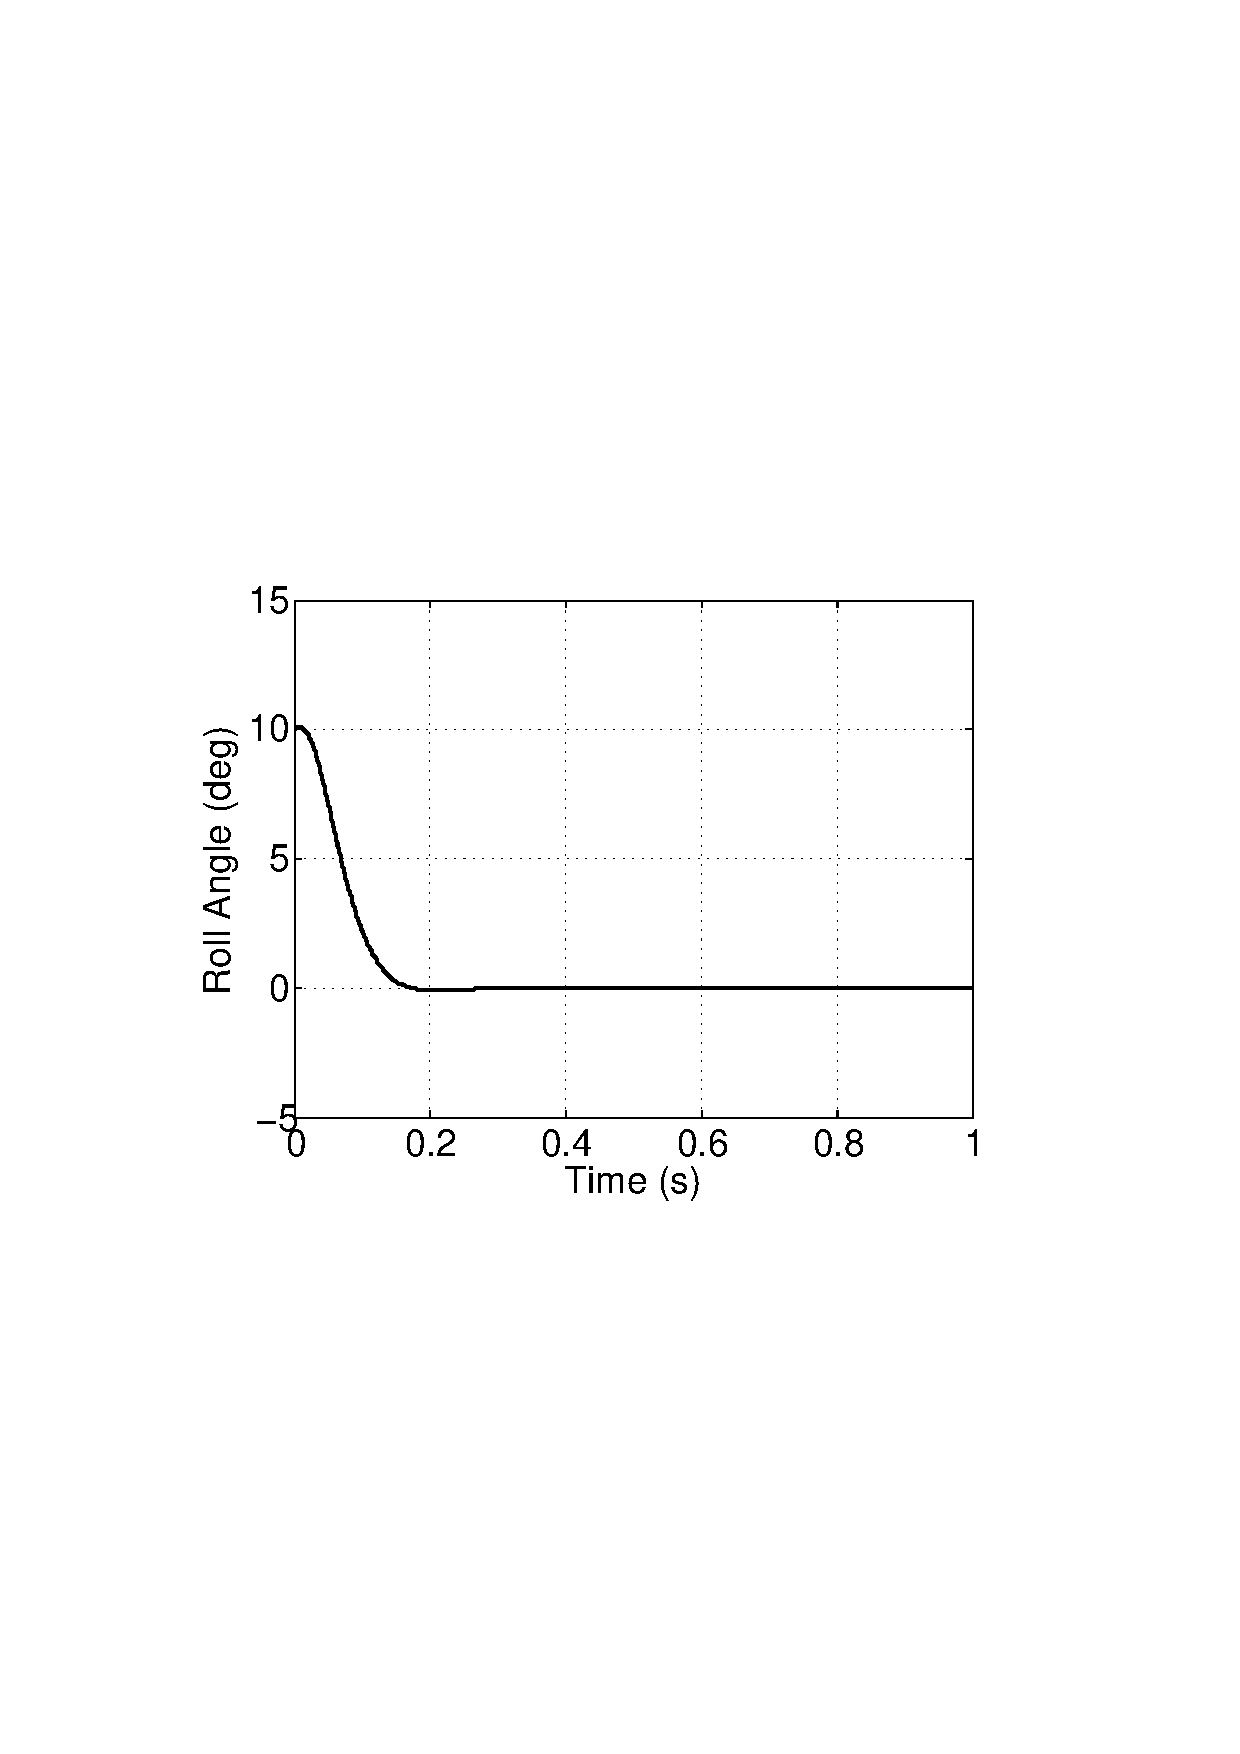
\includegraphics[width=8.4cm]{fig2a}}
	\subfigure[Output Response]{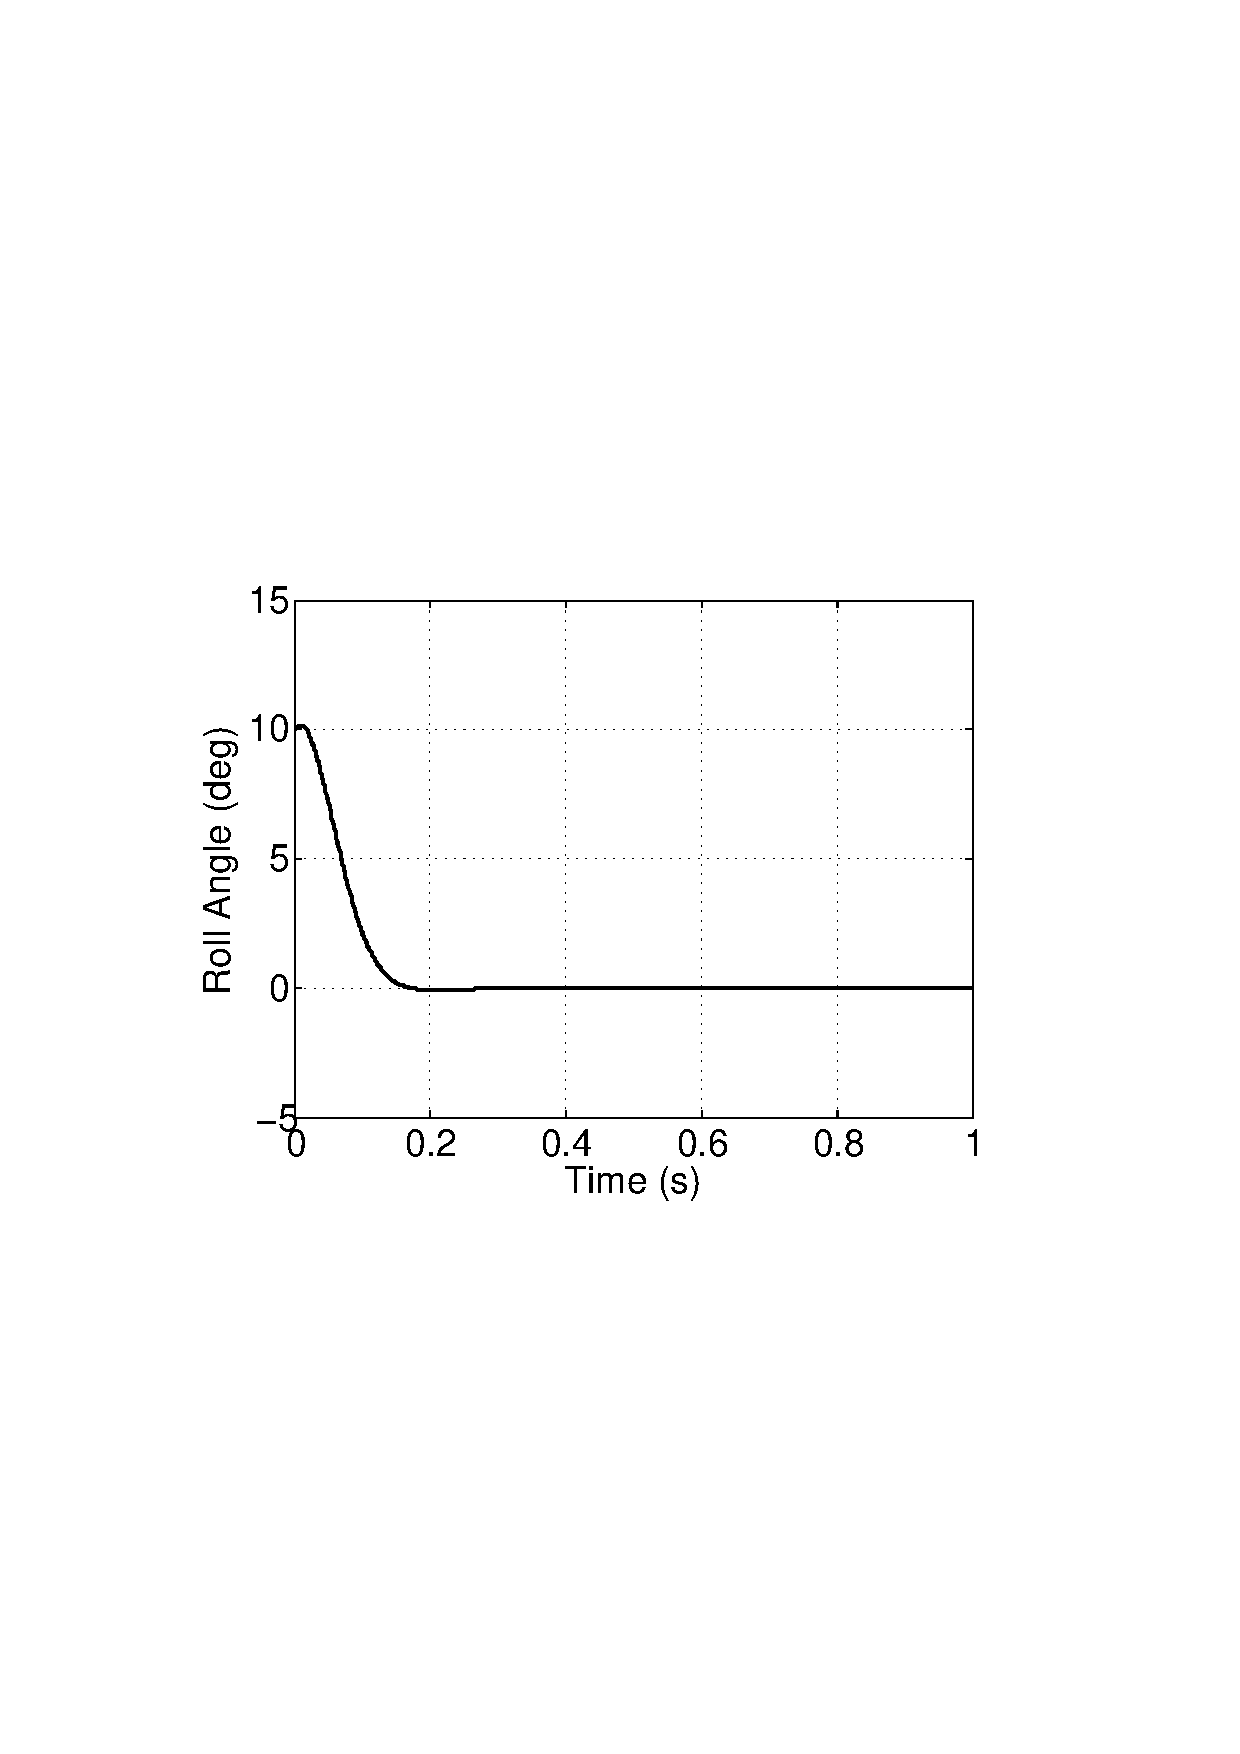
\includegraphics[width=4cm]{fig8a}}
	%\includegraphics[width=8.4cm]{fig3a}    % The printed column width is 8.4 cm.
	%\caption{Output response}
	%\end{subfigure}
%
	%\begin{subfigure}
	\subfigure[Control Effort]{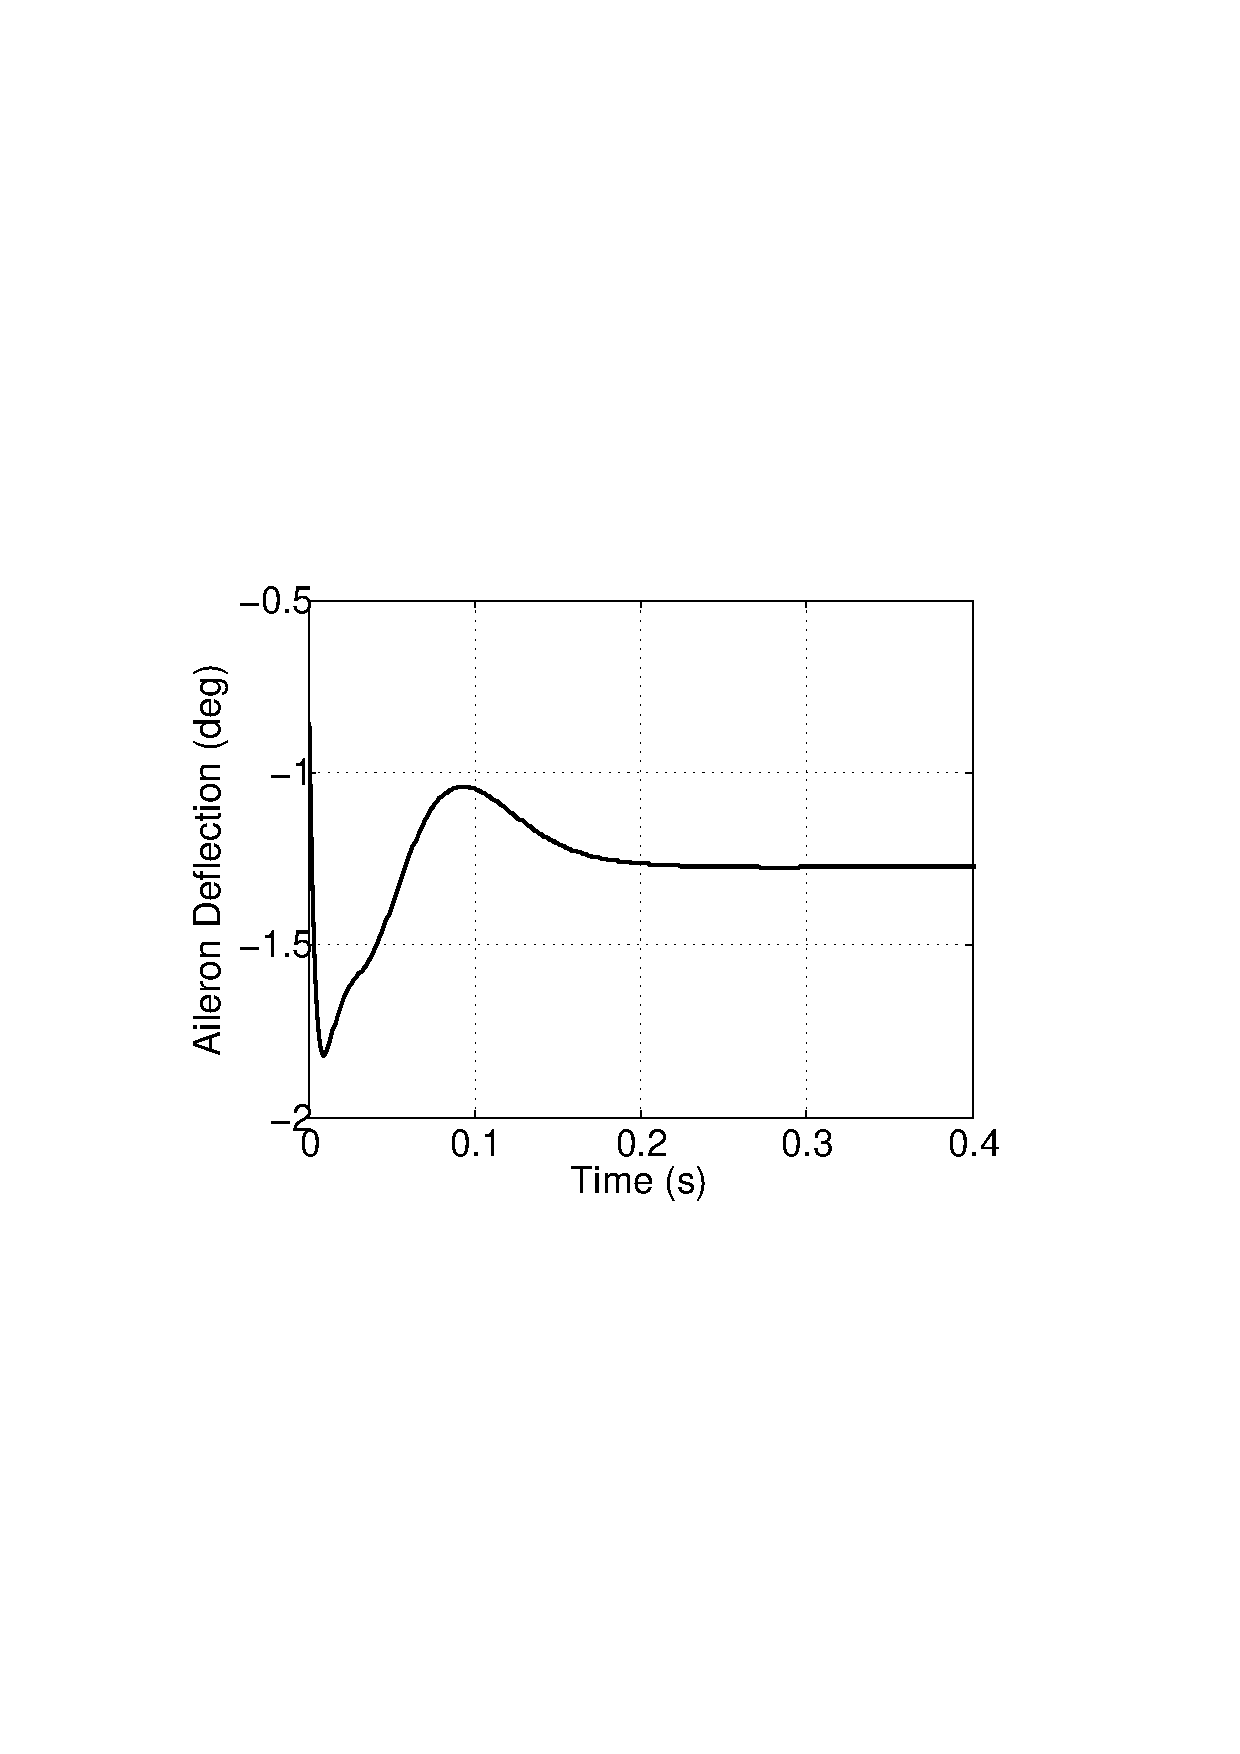
\includegraphics[width=4cm]{fig8b}}
	%\includegraphics[width=8.4cm]{fig3b}    % The printed column width is 8.4 cm.
	%\caption{Control Effort}
	%\end{subfigure}
	\subfigure[Disturbance Estimation]{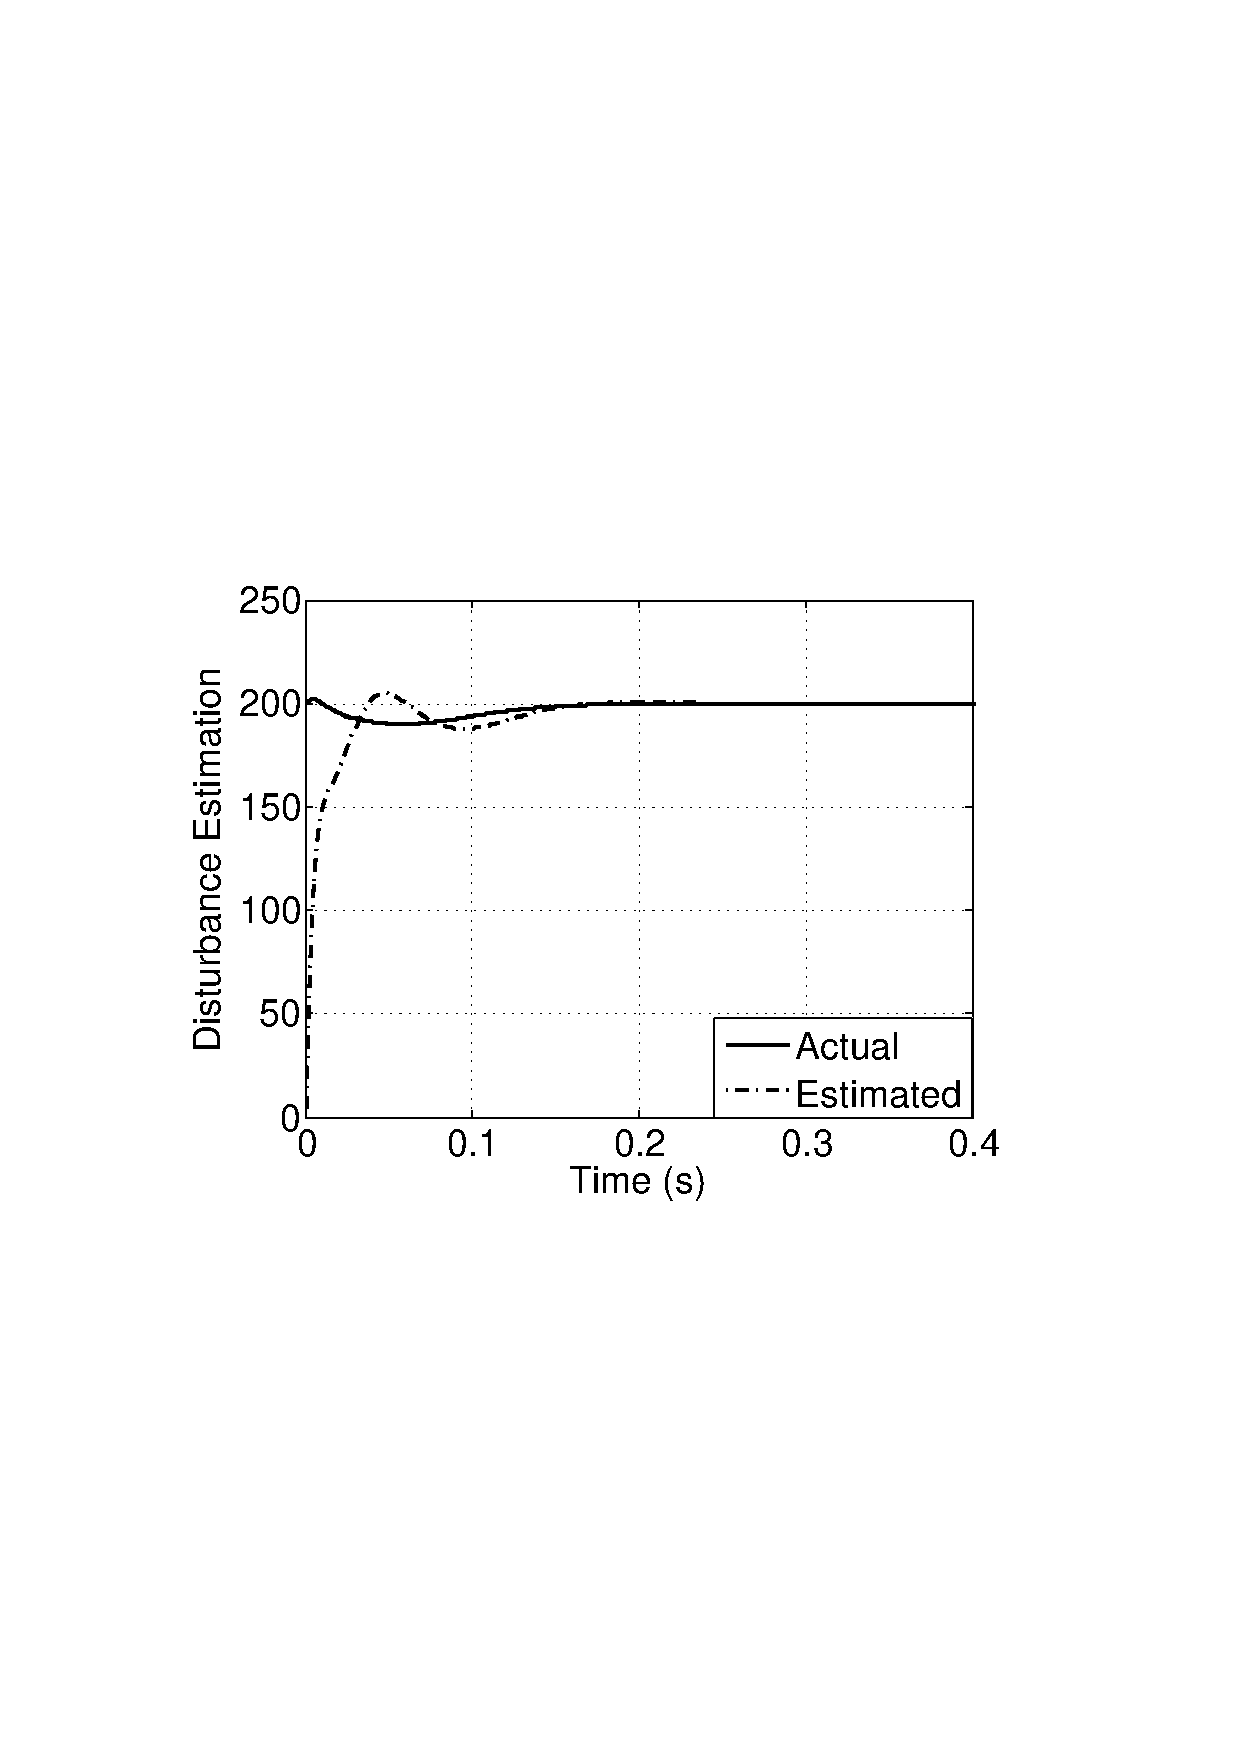
\includegraphics[width=4cm]{fig8c}}
	\subfigure[$\delta$ vs $\delta_c$]{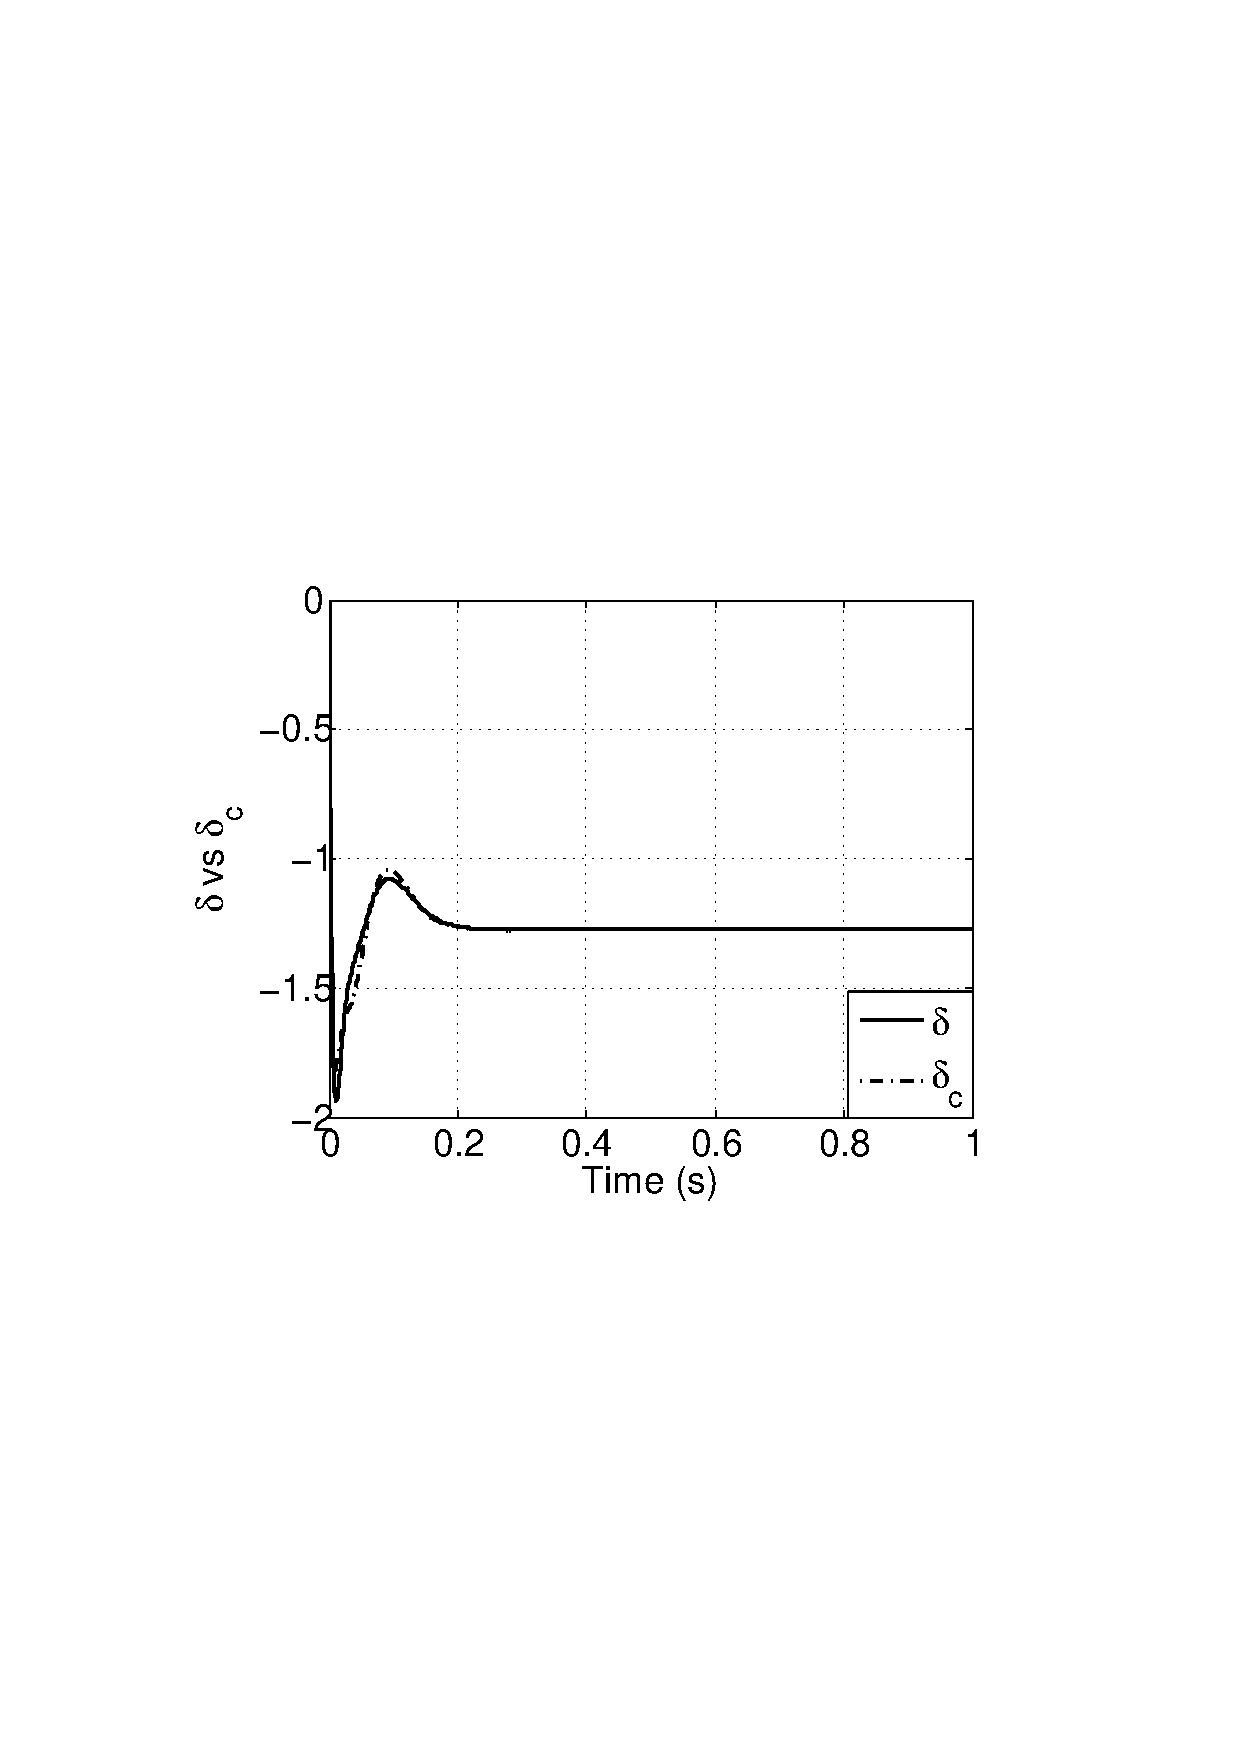
\includegraphics[width=4cm]{fig8d}}
	\caption{Performance with Method 2} 
\label{fig7}
\end{center}
\end{figure}
%---------------------------------------------------------------------------------------------------------------------------------
It can be observed in Fig. 7d, that the compensator (\ref{eq18}) has been successful in its attempt to make $\delta$ track $\delta_c$. 
While this approach satisfies all criteria of the desired performance, its main drawback lies in its dependence on the availability of the derivatives of $\delta$ and $\delta_c$. While the requirement for their availability was met with, solely for simulation purposes, their availability cannot be assured in real-life situations.
%---------------------------------------------------------------------------------------------------------------------------------
\subsection{Method 3: Using Compensator Form 2}
To eliminate the need for the derivatives of $\delta$ and $\delta_c$, another strategy for designing an actuator compensator is proposed, which not only compensates the actuator lag, but also reduces the number of derivatives required. As referred from \cite{ogata2010}, the block diagram schematic is as shown in Fig. 8.
% ---------------------------------------------------Figure9----------------------------------------------------------------------
\begin{figure}[h]
\begin{center}
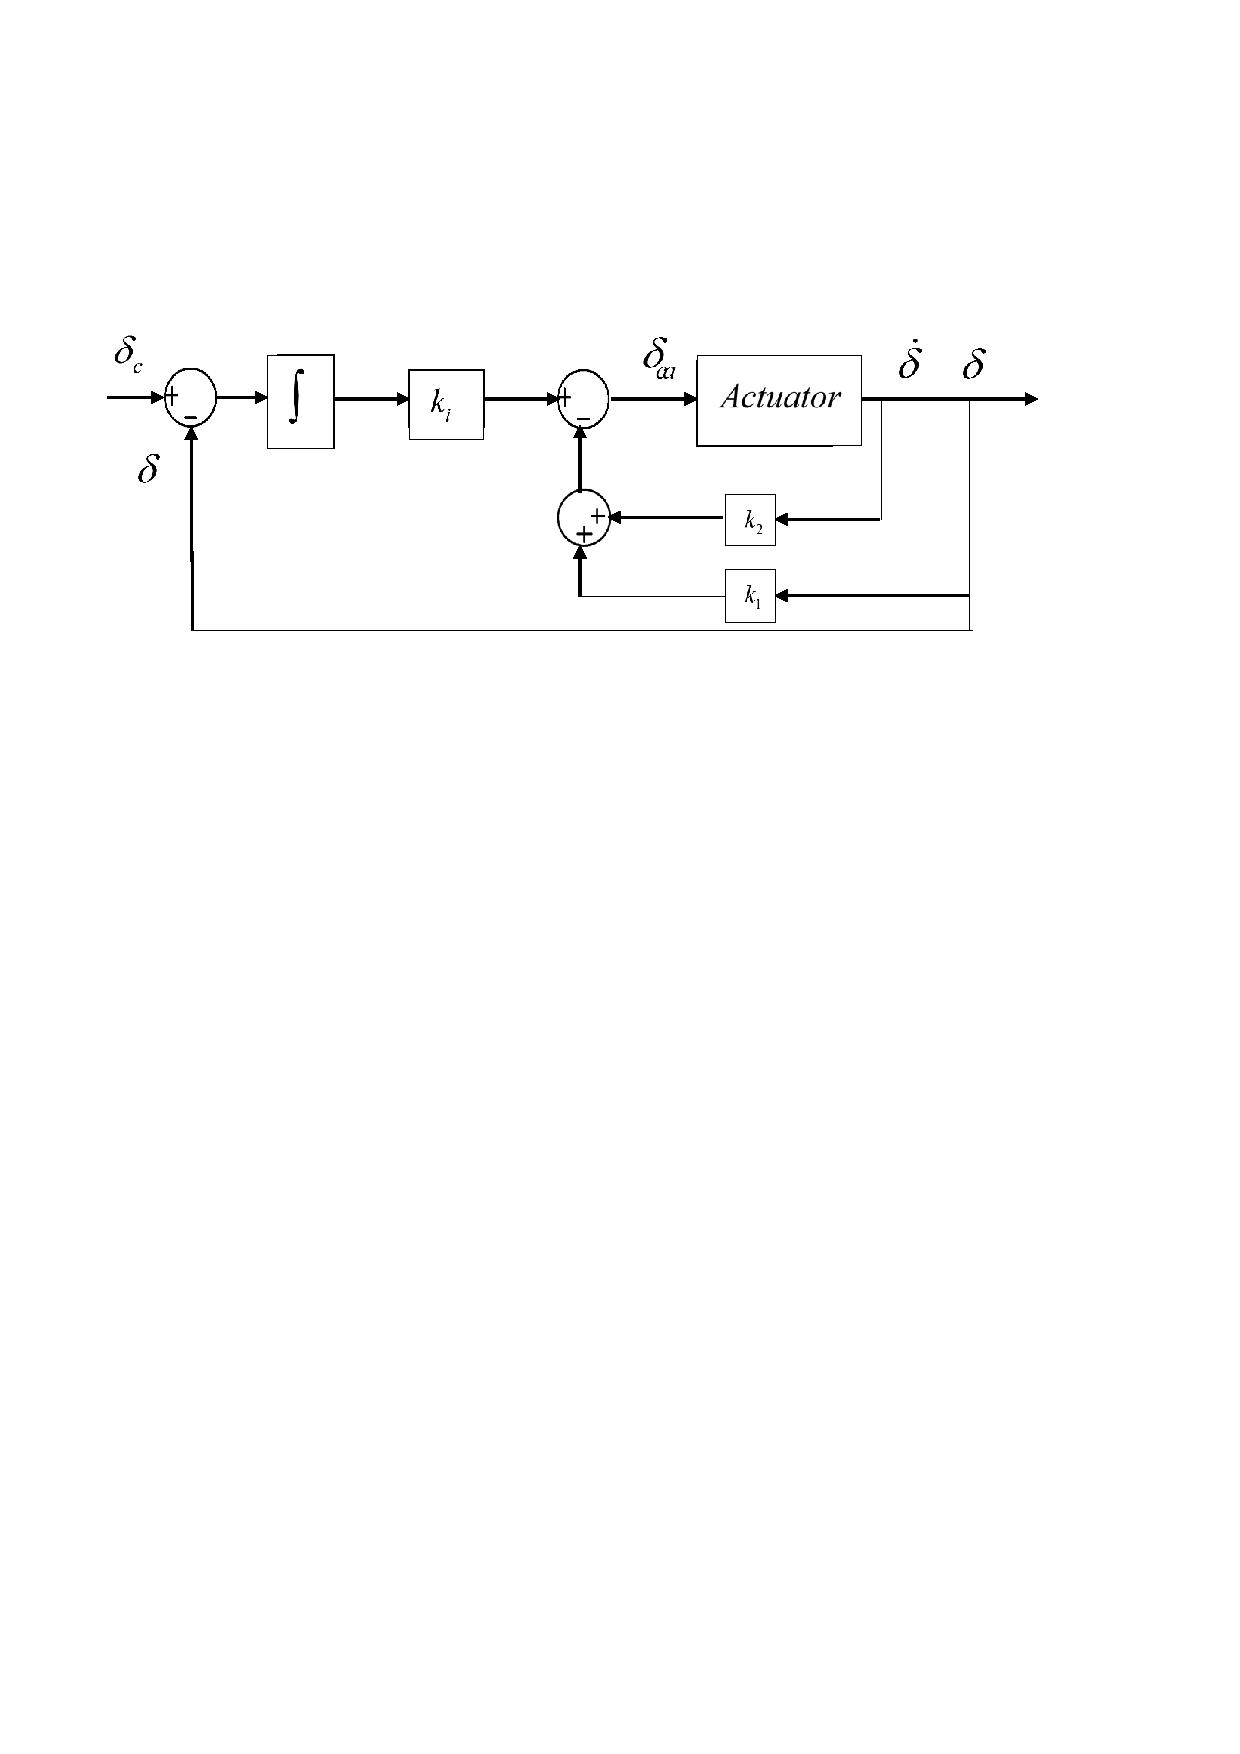
\includegraphics[width=8.4cm]{fig9}   % The printed column width is 8.4 cm.
\caption{Block Diagram Schematic for Method 3} 
\label{fig8}
\end{center}
\end{figure}
%----------------------------------------------------------------------------------------------------------------------------------------------
From Fig. 8, the expression for compensated actuator input $\delta_{ca}$ can be expressed as ;
%
\begin{equation}
\delta_{ca}=-k_1\delta-k_2\dot{\delta}+k_i\int[\delta_c-\delta]dt
\label{eq21}
\end{equation}
%
The transfer function of the second order actuator, as shown in Fig. 3, can be written as;
%
\begin{equation}
%\delta_{ca}={{1}\over{\omega^2_A}}(\nu_a+u_{na})
{{\delta (s)}\over{\delta_c(s)}} = {{b}\over{s^2 + as + b}}
\label{eq22}
\end{equation}
%
with $b=\omega_A^2$ and $a=2\zeta_A\omega_A$. The actuator dynamics can be re-written in the state space model as follows;
%
\begin{eqnarray}
\dot{x} &=& Ax+Bu \nonumber \\
y &=& Cx
\label{eq23}
\end{eqnarray}
%
where A, B and C are the matrices of the system and are given by
$$
A=\left[
\begin{array}{cccc}
0 & 1\\
-b & -a\\
\end{array}\right]; 
%$$
%$$
B=\left[
\begin{array}{cccc}
0 \\
b\\
\end{array}\right]; 
%$$
%$$
C=\left[
\begin{array}{cccc}
1 & 0\\
0 & 1\\
\end{array}\right]
$$
%
With the state variables $x_1$ and $x_2$ being $\delta$ and $\dot{\delta}$, respectively, following \cite{ogata2010}, the control input $u$ is defined as follows;
%
\begin{equation}
u= \delta_{ca}= -k_1\delta -k_2\dot{\delta} +k_i \int{(\delta_c-\delta)}dt
\label{eq24}
\end{equation}
%
%where $k_i$ is the integral gain and $K$ is a matrix defined to be equal to 
%
%$$
%K=\left[
%\begin{array}{cccc}
%k_1 & k_2 \\
%\end{array}\right]
%$$
%
To determine the values of user defined gains $k_1$, $k_2$ and $k_i$, we need to determine the desired and the actual characteristic equations for the closed loop system comprising of the actuator and its compensator. The desired characteristic equation for this system is of the form $(s^2+ 2\zeta_d\omega_ds+ \omega_d^2)(s+ \zeta_d\omega_d)=0$ for a desired settling time and damping factor. To derive the actual characteristic equation for this system, following \cite{ogata2010}, we first need to define matrices $\hat A$, $\hat B$, $\hat K$;
%
$$
\hat A=\left[
\begin{array}{cc}
A & 0\\
-C & 0\\
\end{array}\right]; 
%$$
%$$
\hat B=\left[
\begin{array}{c}
B\\
0\\
\end{array}\right]; 
%$$
%$$
\hat K=\left[
\begin{array}{ccc}
k_1 & k_2 & k_i\\
\end{array}\right]
$$
% 
Computing $sI-(\hat A-\hat B\hat K)=0$ results in the actual characteristic equation of the form;
%
\begin{equation}
s^3+s^2(a+bk_2)+s(b+bk_1)+bk_i=0
\label{eq25}
\end{equation}
%
From the desired and the actual characteristic equation, we can evaluate the values of $k_1$, $k_2$ and $k_i$ .

To determine the desired characteristic equation, a damping factor of 0.8 is chosen. The desired settling time for the actuator compensator-actuator system now needs to be determined, the choice of which bears a close relationship with the actuator parameters. From the knowledge of the parameters of actuator: $\omega_A=100$ rad/s and $\zeta_A = 0.8$, the settling time for the actuator is 50 ms. Since the compensator dynamics need to be faster than the actuator dynamics, by rule of thumb we choose a desired settling time to be $1/4$ times the actuator settling time, i.e. 12.5 ms, For these values of settling time and damping factor, the desired characteristic equation is derived and compared with the actual characteristic equation to give values of $k_1$, $k_2$ and $k_i$, as discussed subsequently. 


\subsubsection{Performance Analysis of UDE based controller with actuator compensation using Method 3}
Simulation is carried out with simulation parameters as per Table. 1 and an external disturbance equal to $d_{ext}$. As stated before, simulations were carried out for a desired settling time of 12.5 ms for the actuator compensator-actuator system, retaining the value of $\tau$ as 0.01. For this value of desired settling time, with damping ratio of 0.8, $k_1$, $k_2$ and $k_i$ were calculated to be 35.48, 0.083, 5120, respectively. Simulation results are shown in Fig. 9.
% ---------------------------------------------------Figure10---------------------------------------------------------------------
\begin{figure}[h]
\begin{center}
	%\begin{subfigure}
	%\subfigure[Output Response]{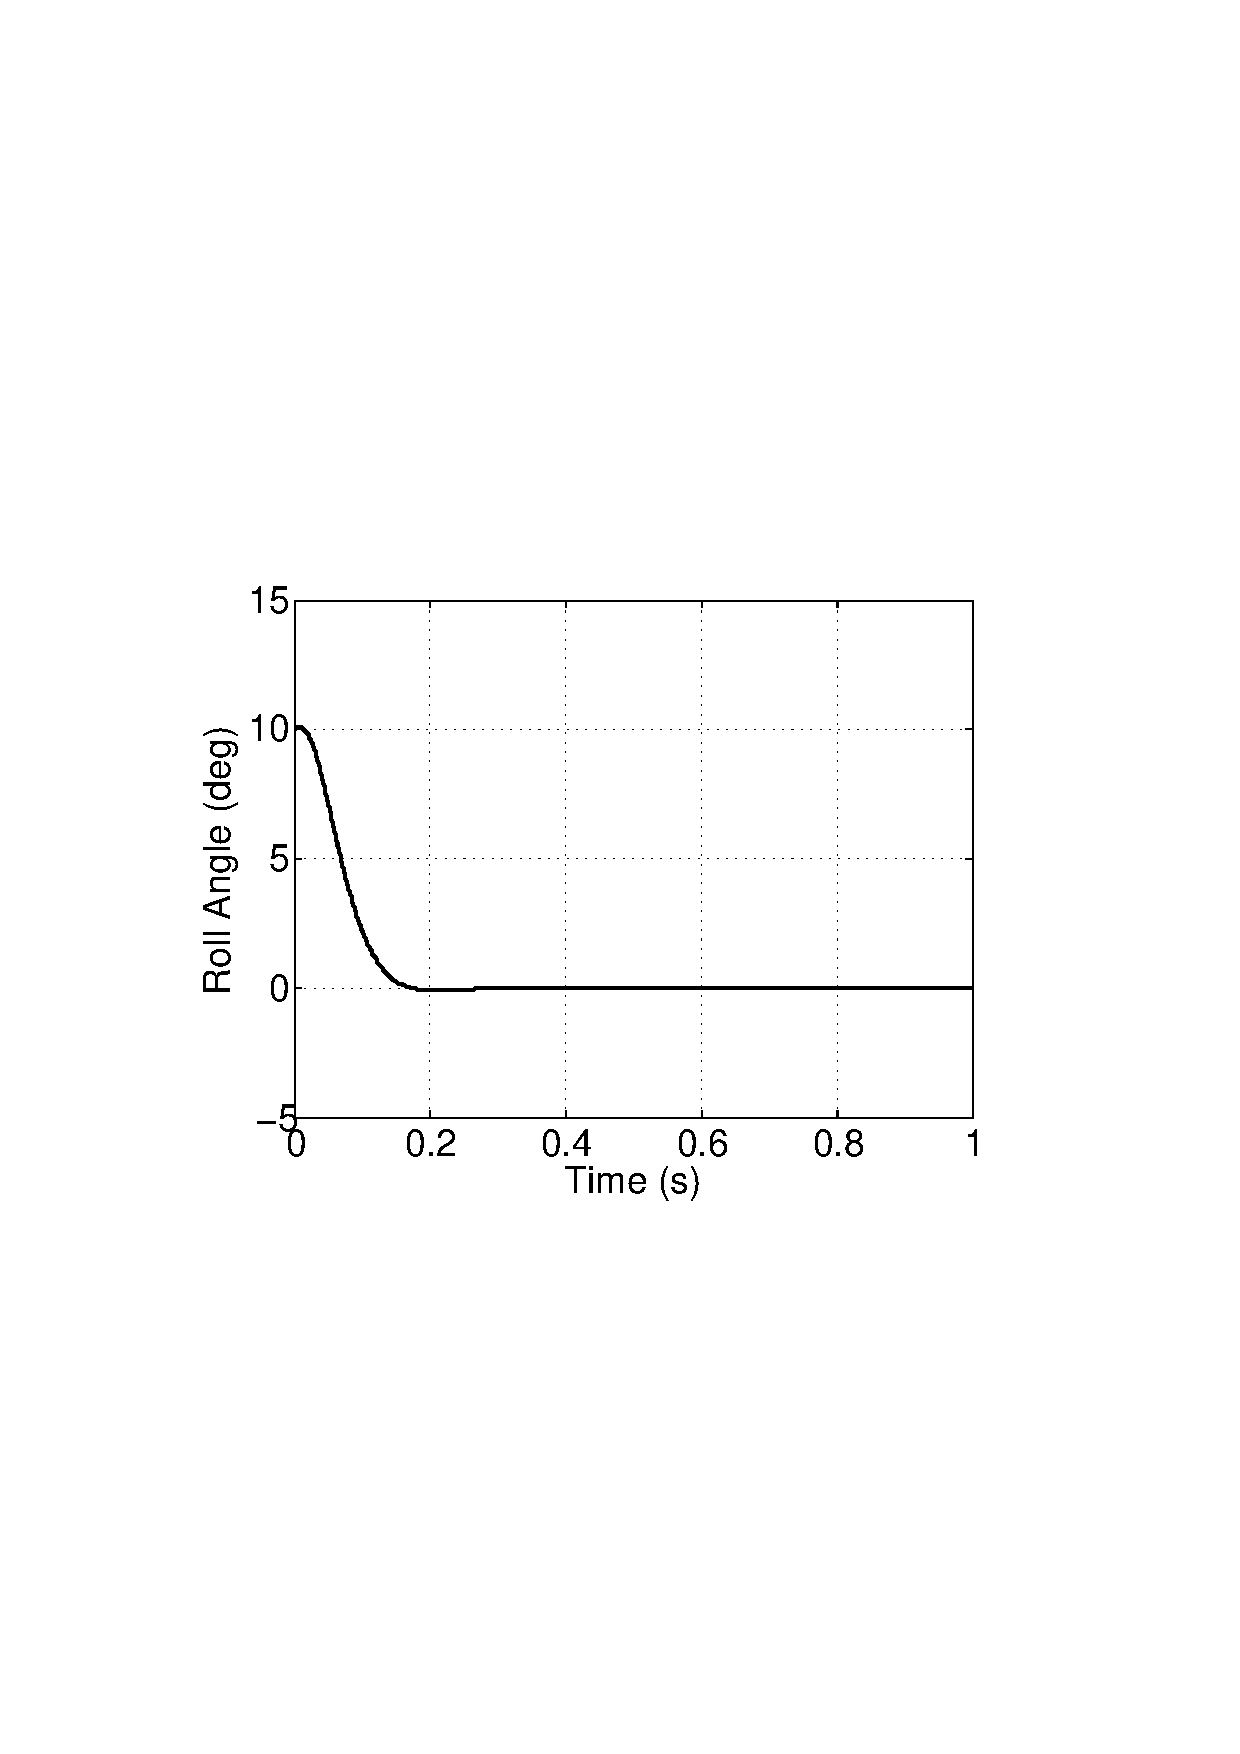
\includegraphics[width=8.4cm]{fig2a}}
	\subfigure[Output Response]{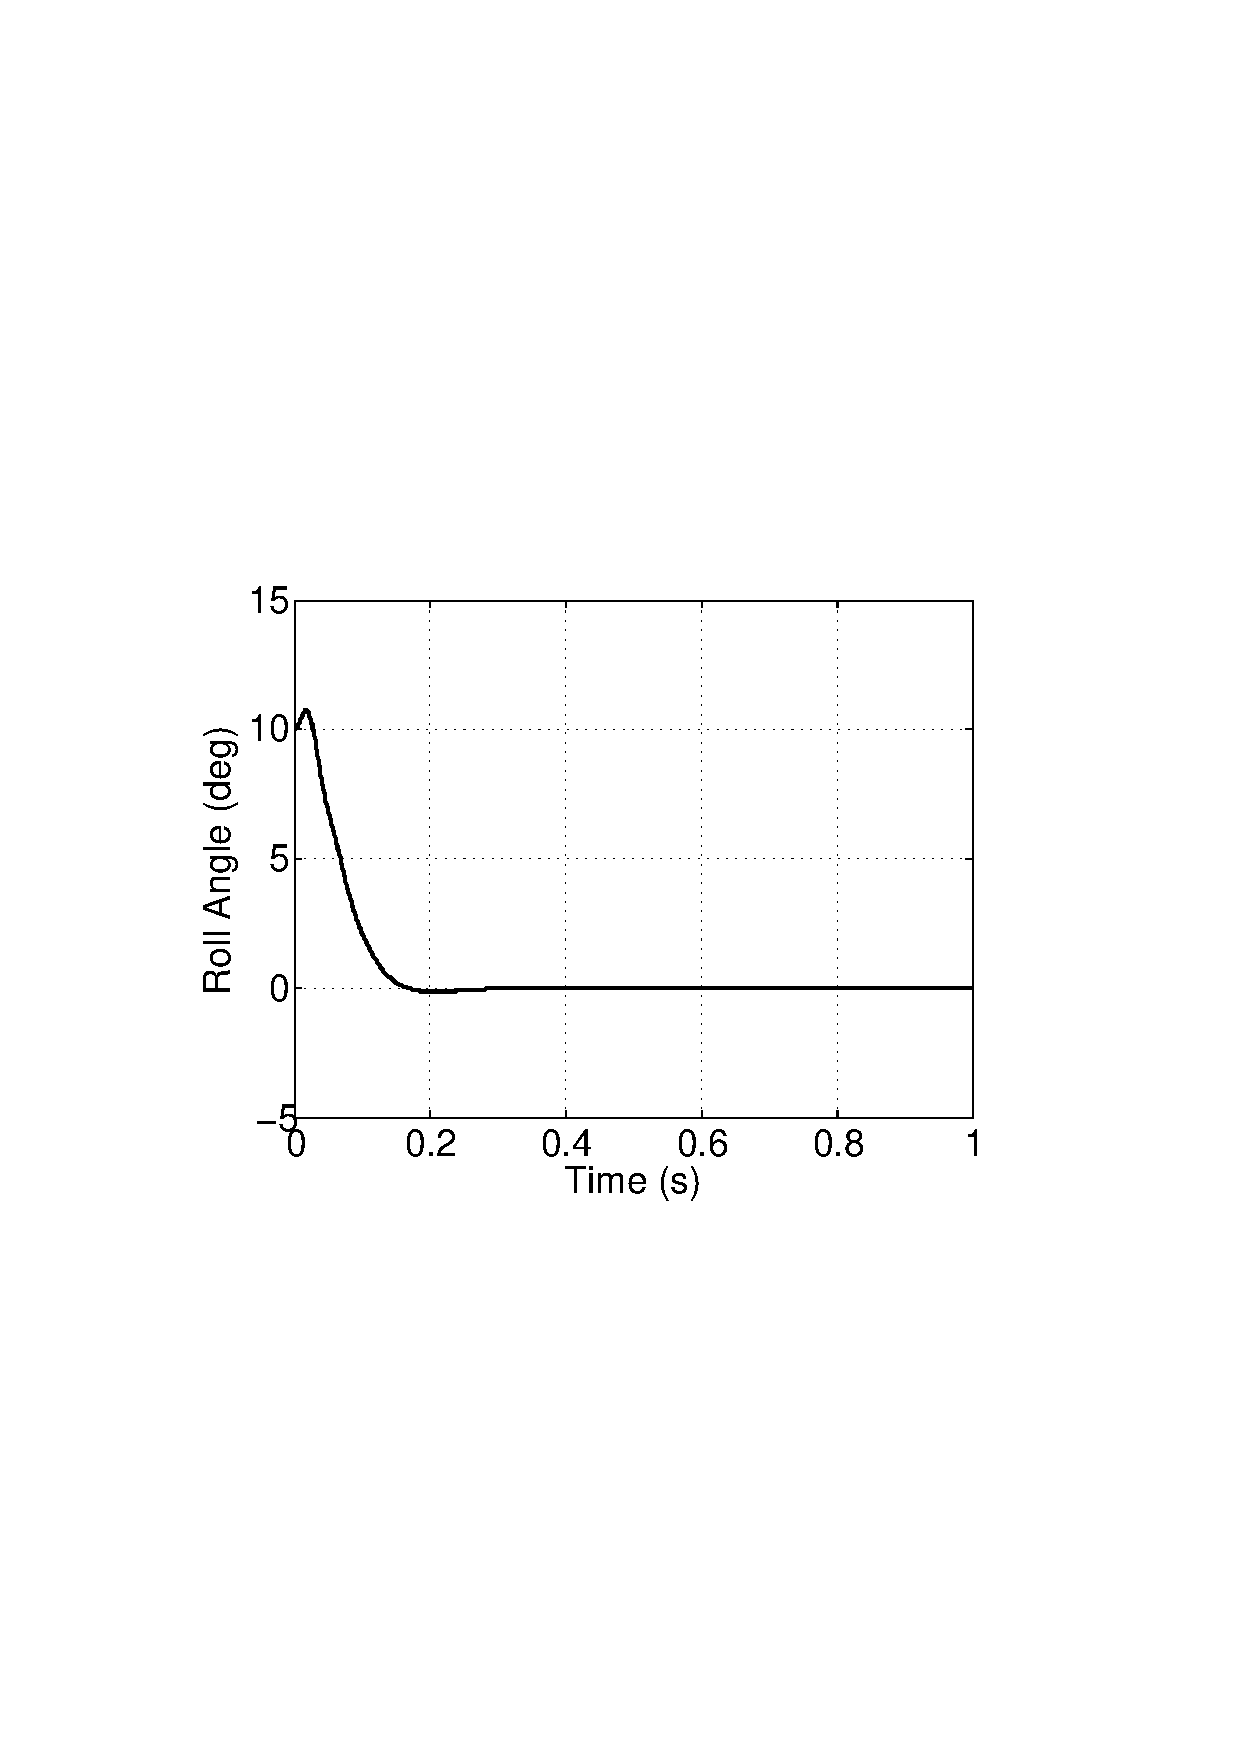
\includegraphics[width=4cm]{fig10a}}
	%\includegraphics[width=8.4cm]{fig3a}    % The printed column width is 8.4 cm.
	%\caption{Output response}
	%\end{subfigure}
%
	%\begin{subfigure}
	\subfigure[Control Effort]{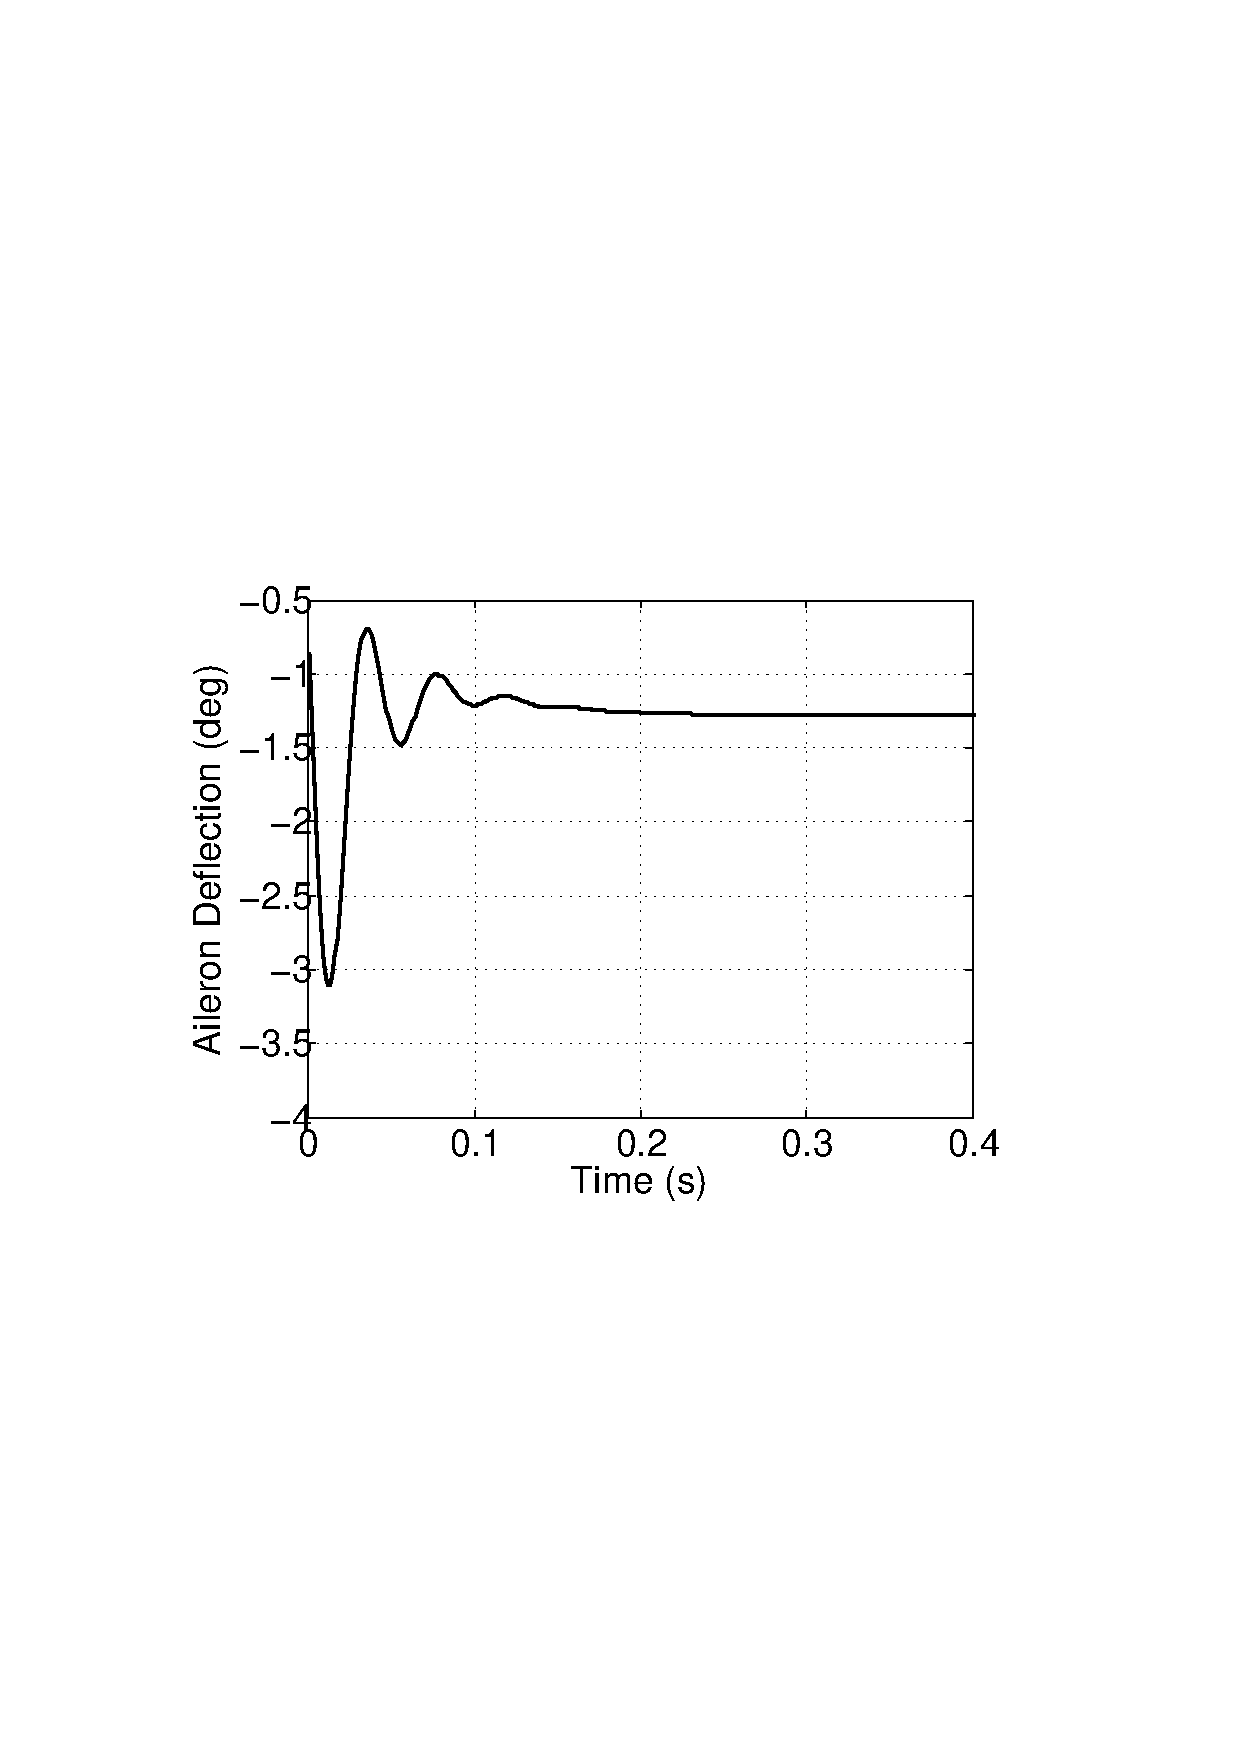
\includegraphics[width=4cm]{fig10b}}
	%\includegraphics[width=8.4cm]{fig3b}    % The printed column width is 8.4 cm.
	%\caption{Control Effort}
	%\end{subfigure}
	\subfigure[Disturbance Estimation]{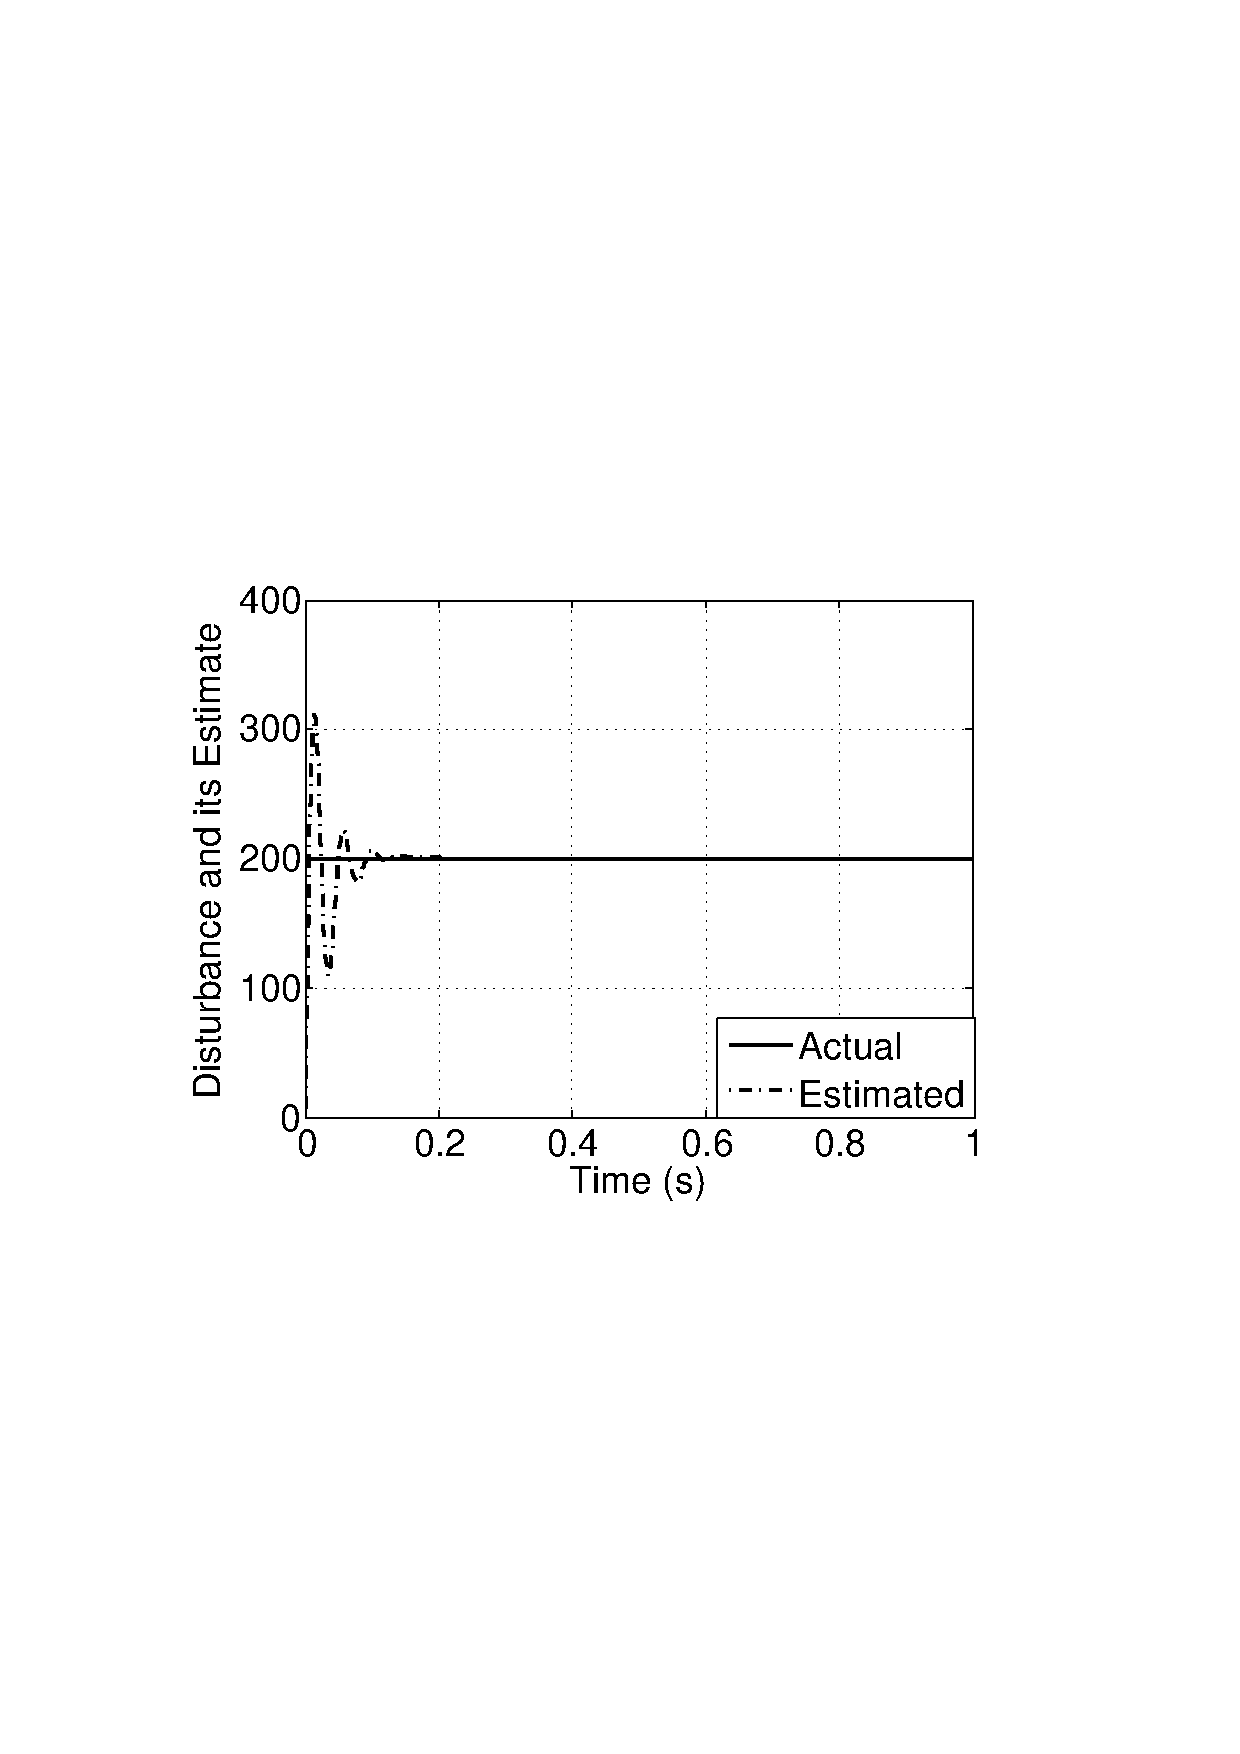
\includegraphics[width=4cm]{fig10c}}
	%
	\subfigure[$\delta$ vs $\delta_c$]{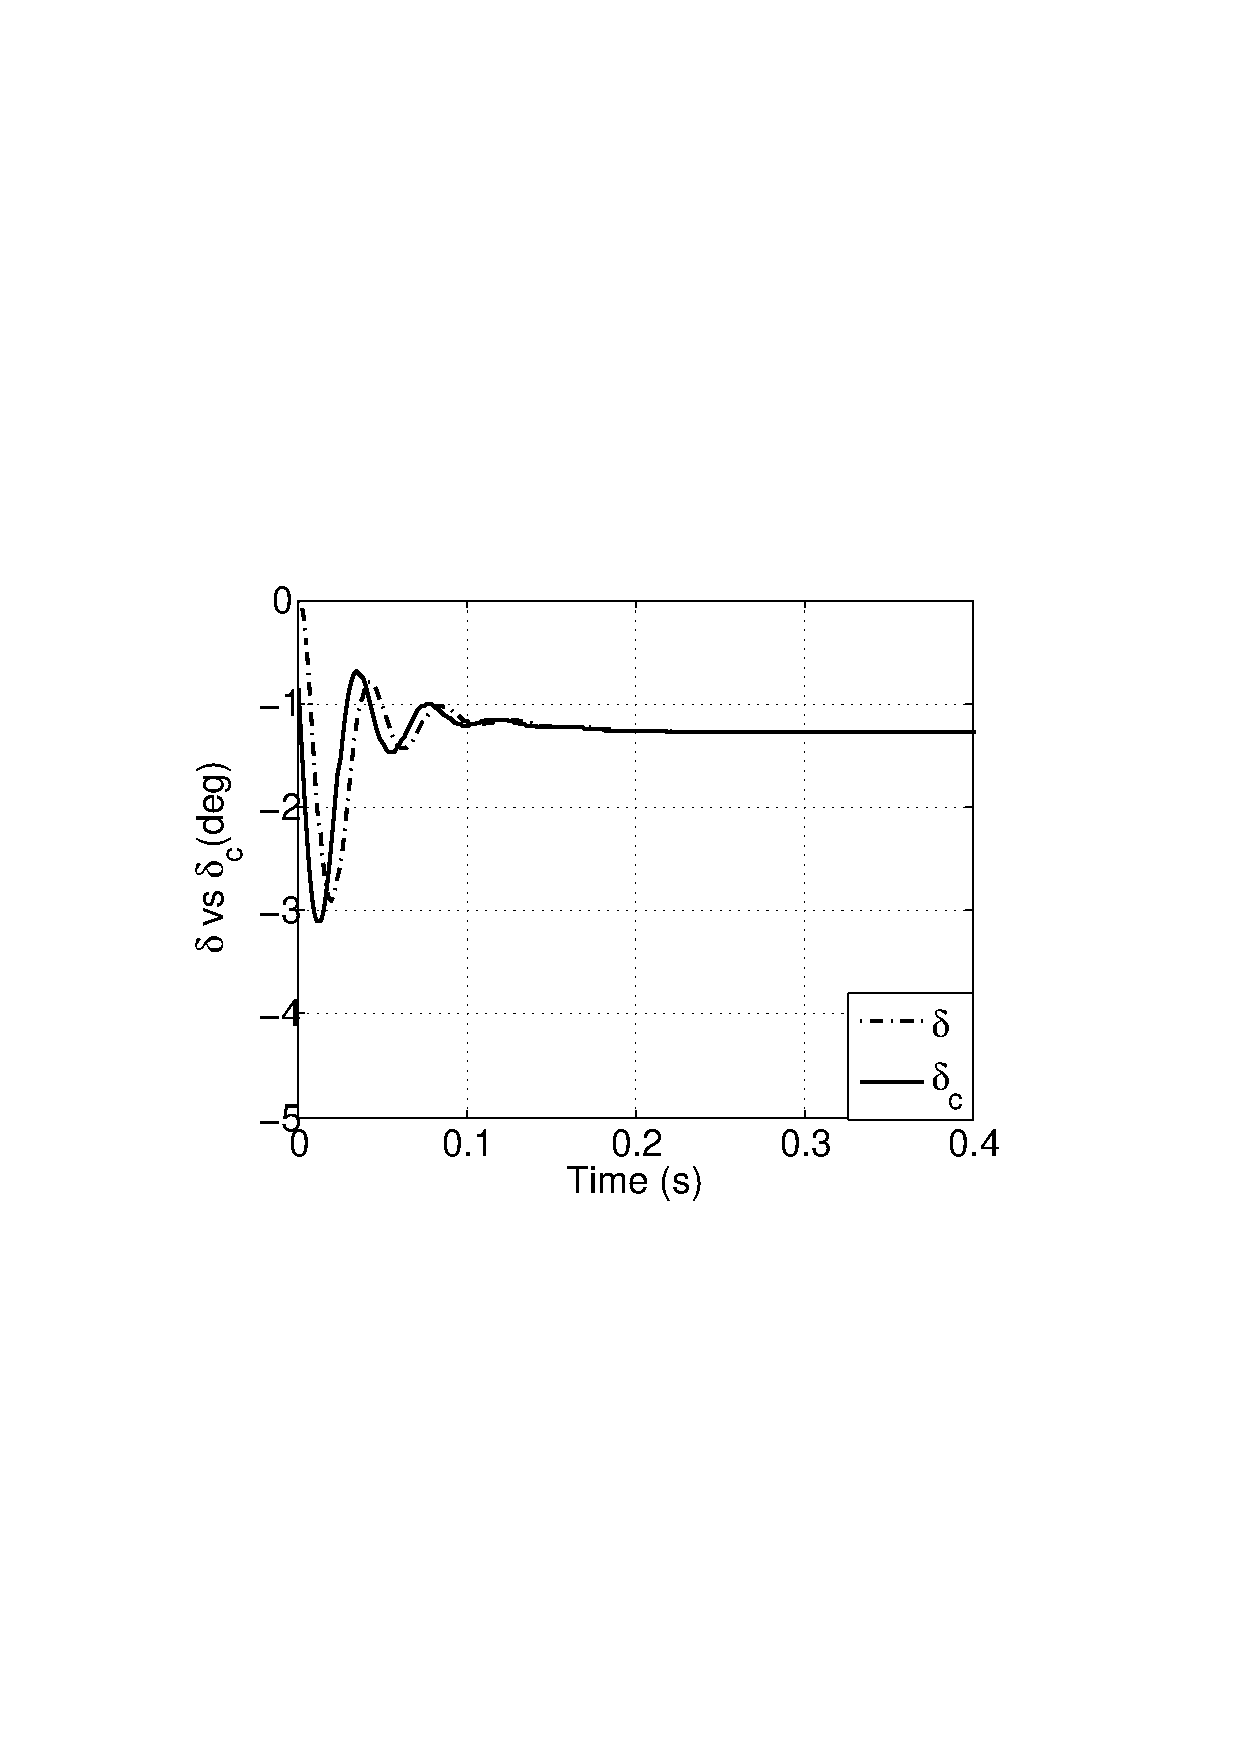
\includegraphics[width=4cm]{fig10d}}
	\caption{Performance with Method 3 ($k_1= 35.48, k_2= 0.083, k_i= 5120$)} 
\label{fig9}
\end{center}
\end{figure}
%
From Fig. 9a, it can be observed that the roll angle $\phi$ has settled down to zero, as desired. The output response shows a small overshoot. It can be seen from Fig. 9d, that $\delta$ tracks $\delta_c$ as desired. 
It can thus be concluded that by proper choice of $k_1$, $k_2$ and $k_i$, the delay created by the actuator can be compensated. When a desired settling time of 25 ms was chosen with corresponding values $k_1$, $k_2$ and $k_i$, the performance was observed to be similar to Method 1 (Fig. 5 refers).
Few more trials were carried out to explore the relation between the choice of $\tau$ and desired settling time of the actuator compensator-actuator system. It was observed that for a given damping ratio, say 0.8, the relation between $\tau$ and settling time for the error dynamics ($t_s$) can be expressed as $\tau=1.25 t_s$. Following this analogy, keeping $\tau=0.01$, the desired settling time was computed to be 7.96 ms. $k_1$, $k_2$ and $k_i$ were then calculated to be 88.89, 0.137 and 19800, respectively. Further, an uncertainty of -30 \% in $\omega_{RR}$ and +30 \% in $K_{\delta}$ along with $d_{ext}$ were introduced. Simulation results for this choice, are shown in Fig. 10, which indicate satisfactory performance.
% ---------------------------------------------------Figure11---------------------------------------------------------------------
\begin{figure}[h]
\begin{center}
	%\begin{subfigure}
	%\subfigure[Output Response]{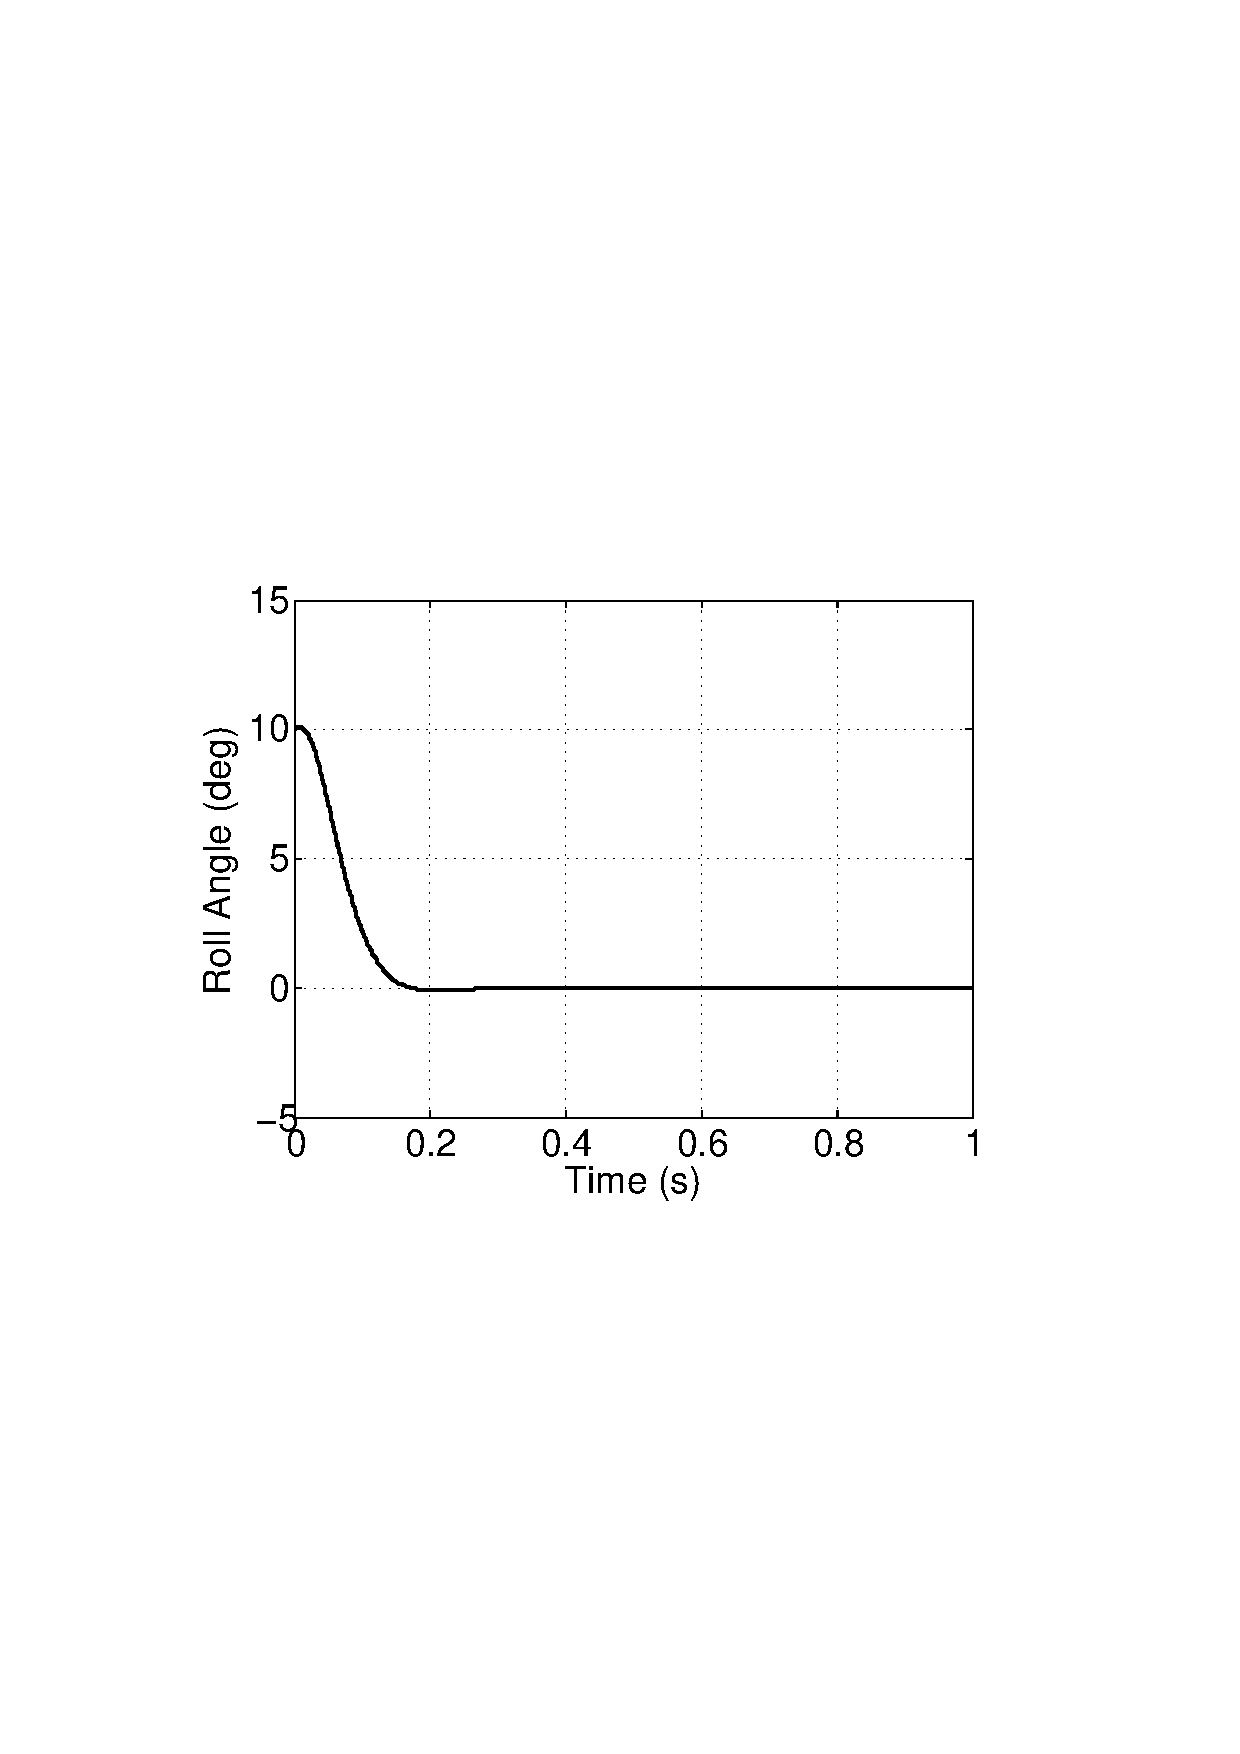
\includegraphics[width=8.4cm]{fig2a}}
	\subfigure[Output Response]{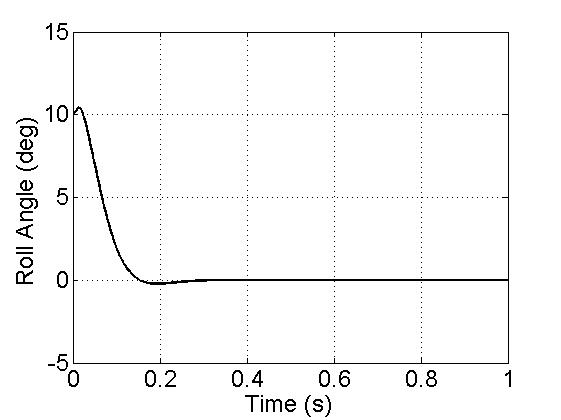
\includegraphics[width=4cm]{fig11a}}
	%\includegraphics[width=8.4cm]{fig3a}    % The printed column width is 8.4 cm.
	%\caption{Output response}
	%\end{subfigure}
%
	%\begin{subfigure}
	\subfigure[Control Effort]{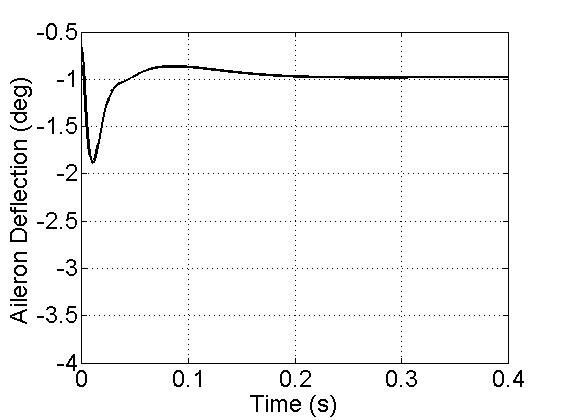
\includegraphics[width=4cm]{fig11b}}
	%\includegraphics[width=8.4cm]{fig3b}    % The printed column width is 8.4 cm.
	%\caption{Control Effort}
	%\end{subfigure}
	\subfigure[Disturbance Estimation]{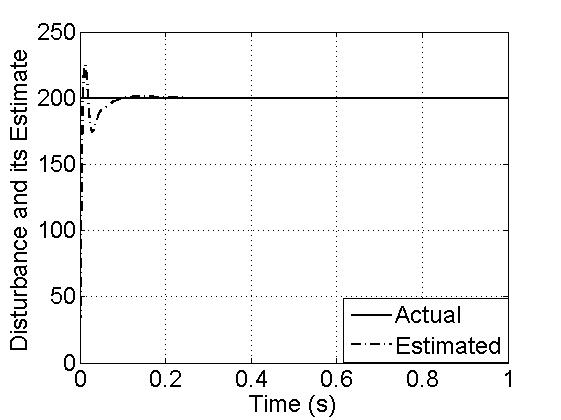
\includegraphics[width=4cm]{fig11c}}
	%
	\subfigure[$\delta$ vs $\delta_c$]{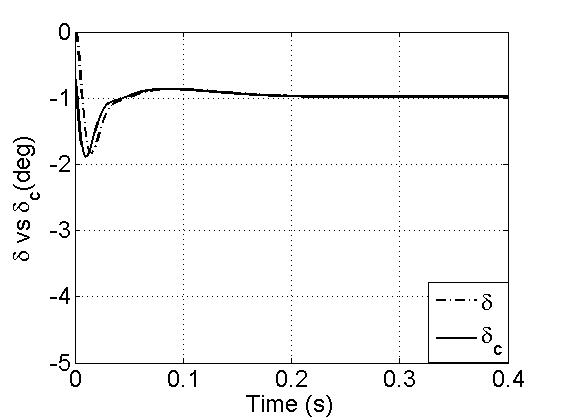
\includegraphics[width=4cm]{fig11d}}
	\caption{Performance with Method 3 ($k_1= 88.89, k_2= 0.137, k_i= 19800$)}
\label{fig10}
\end{center}
\end{figure}
%
This approach when compared to the previous two approaches, yields better results, while eliminating the need for $\ddot{\delta}$, $\ddot{\delta_c}$ and even $\dot{\delta_c}$. To demonstrate the validity of the proposed Method 3 in practical situations, constraints were imposed on $\delta$ and $\dot{\delta}$ to the tune of +/- 24 deg and +/- 250 deg/s, respectively. While simulating Fig.10, it was found that the obtained values were within specified limits. Effects of dead zone, backlash of a practical actuator and measurement noise on the performance, have been assigned for future study.  
%---------------------------------------------------------------------------------------------------------------------------------
\section{Conclusion}
%In this work, the strategy of uncertainty and disturbance estimator (UDE) was employed in the design of a robust roll autopilot. Design of a robust UDE based law for the roll dynamics assuming ideal actuator was carried out first, followed by the presentation of effects of second order actuator in the performance. By tuning the filter time constant, the performance of UDE based controller for robustness and actuator compensation was found to be acceptable, though required improvement. To achieve this, two forms of compensator were proposed and evaluated. It was found that Compensator Form 2 gave the desired results at the same time reducing the requirement of derivatives of the control effort.
%
In this work, the strategy of UDE was employed in the design of a robust roll autopilot with actuator compensation. Design assuming ideal actuator followed by the effects of second order actuator in the performance have been presented. By tuning the filter time constant, the performance of UDE based controller for robustness and actuator compensation was found to be acceptable, though required improvement. To achieve this, two forms of compensator were proposed and evaluated. It was found that Compensator Form 2 gave the desired results at the same time reducing the requirement of derivatives of the control effort. Our future work would involve further investigation into the role of filter time constant ($\tau$) in actuator compensation. Design of UDE based control law to cater to time varying uncertainties and disturbances along with actuator compensation, is another area to be focused in future. Applicability of the proposed methods for non-linear roll dynamics would also be explored in our future work.


%%------------------------------------------------------------------------------------------------------------------------------------------------------------------------------------------
%%\subsection{Subsection Heading Here}
%%Subsection text here.
%%
%%
%%\subsubsection{Subsubsection Heading Here}
%%Subsubsection text here. \cite{song2002}.
%
%
%% An example of a floating figure using the graphicx package.
%% Note that \label must occur AFTER (or within) \caption.
%% For figures, \caption should occur after the \includegraphics.
%% Note that IEEEtran v1.7 and later has special internal code that
%% is designed to preserve the operation of \label within \caption
%% even when the captionsoff option is in effect. However, because
%% of issues like this, it may be the safest practice to put all your
%% \label just after \caption rather than within \caption{}.
%%
%% Reminder: the "draftcls" or "draftclsnofoot", not "draft", class
%% option should be used if it is desired that the figures are to be
% displayed while in draft mode.
%
%\begin{figure}[!t]
%\centering
%\includegraphics[width=2.5in]{myfigure}
% where an .eps filename suffix will be assumed under latex, 
% and a .pdf suffix will be assumed for pdflatex; or what has been declared
% via \DeclareGraphicsExtensions.
%\caption{Simulation results for the network.}
%\label{fig_sim}
%\end{figure}

% Note that IEEE typically puts floats only at the top, even when this
% results in a large percentage of a column being occupied by floats.


% An example of a double column floating figure using two subfigures.
% (The subfig.sty package must be loaded for this to work.)
% The subfigure \label commands are set within each subfloat command,
% and the \label for the overall figure must come after \caption.
% \hfil is used as a separator to get equal spacing.
% Watch out that the combined width of all the subfigures on a 
% line do not exceed the text width or a line break will occur.
%
%\begin{figure*}[!t]
%\centering
%\subfloat[Case I]{\includegraphics[width=2.5in]{box}%
%\label{fig_first_case}}
%\hfil
%\subfloat[Case II]{\includegraphics[width=2.5in]{box}%
%\label{fig_second_case}}
%\caption{Simulation results for the network.}
%\label{fig_sim}
%\end{figure*}
%
% Note that often IEEE papers with subfigures do not employ subfigure
% captions (using the optional argument to \subfloat[]), but instead will
% reference/describe all of them (a), (b), etc., within the main caption.
% Be aware that for subfig.sty to generate the (a), (b), etc., subfigure
% labels, the optional argument to \subfloat must be present. If a
% subcaption is not desired, just leave its contents blank,
% e.g., \subfloat[].


% An example of a floating table. Note that, for IEEE style tables, the
% \caption command should come BEFORE the table and, given that table
% captions serve much like titles, are usually capitalized except for words
% such as a, an, and, as, at, but, by, for, in, nor, of, on, or, the, to
% and up, which are usually not capitalized unless they are the first or
% last word of the caption. Table text will default to \footnotesize as
% IEEE normally uses this smaller \sffamilyfont for tables.
% The \label must come after \caption as always.
%
%\begin{table}[!t]
%% increase table row spacing, adjust to taste
%\renewcommand{\arraystretch}{1.3}
% if using array.sty, it might be a good idea to tweak the value of
% \extrarowheight as needed to properly center the text within the cells
%\caption{An Example of a Table}
%\label{table_example}
%\centering
%% Some packages, such as MDW tools, offer better commands for making tables
%% than the plain LaTeX2e tabular which is used here.
%\begin{tabular}{|c||c|}
%\hline
%One & Two\\
%\hline
%Three & Four\\
%\hline
%\end{tabular}
%\end{table}


% Note that the IEEE does not put floats in the very first column
% - or typically anywhere on the first page for that matter. Also,
% in-text middle ("here") positioning is typically not used, but it
% is allowed and encouraged for Computer Society conferences (but
% not Computer Society journals). Most IEEE journals/conferences use
% top floats exclusively. 
% Note that, LaTeX2e, unlike IEEE journals/conferences, places
% footnotes above bottom floats. This can be corrected via the
% \fnbelowfloat command of the stfloats package.
%
%
%
%
%\section{Conclusion}
%The conclusion goes here.
%
%
%
%
%% conference papers do not normally have an appendix
%
%
%% use section* for acknowledgment
%\section*{Acknowledgment}
%
%
%The authors would like to thank...
%
%
%
%
%
% trigger a \newpage just before the given reference
% number - used to balance the columns on the last page
% adjust value as needed - may need to be readjusted if
% the document is modified later
%\IEEEtriggeratref{8}
% The "triggered" command can be changed if desired:
%\IEEEtriggercmd{\enlargethispage{-5in}}
%
% references section
%
% can use a bibliography generated by BibTeX as a .bbl file
% BibTeX documentation can be easily obtained at:
% http://www.ctan.org/tex-archive/biblio/bibtex/contrib/doc/
% The IEEEtran BibTeX style support page is at:
% http://www.michaelshell.org/tex/ieeetran/bibtex/
%\bibliographystyle{IEEEtran}
% argument is your BibTeX string definitions and bibliography database(s)
%\bibliography{IEEEabrv,../bib/paper}
%
% <OR> manually copy in the resultant .bbl file
% set second argument of \begin to the number of references
% (used to reserve space for the reference number labels box)
\begin{thebibliography}{1}

%\bibitem{IEEEhowto:kopka}
%H.~Kopka and P.~W. Daly, \emph{A Guide to \LaTeX}, 3rd~ed.\hskip 1em plus
  %0.5em minus 0.4em\relax Harlow, England: Addison-Wesley, 1999.
	%
% Reference 1
\bibitem{song2002}
Chanho Sung, and Yoon-Sik Kim, \lq \lq A new approach to motion modeling and autopilot design of skid-to-turn missile," Trans. on Control, Automation, and System Engg, 4(3), Sep 2002, pp. 231-238. 

% Reference 2
\bibitem{kang2009}
S. Kang, and H. J. Kim, \lq \lq Roll-pitch-yaw integrated robust autopilot design for a high angle-of-attack missile," J. of Guidance, Control, and Dynamics, 32(5), Sep-Oct 2009, pp. 1622-1628.

%Reference 3
\bibitem{sirisha2012}
C. V. Sirisha, Ranajit Das, and R. N. Bhattacharjee, \lq \lq Disturbance estimation based roll autopilot design for tactical missiles," Proc. Advances in Control and Optimisation of Dynamic Systems, ACDOS - 2012, pp. 1-5.

%Reference 4
\bibitem{luo2015}
D. Luo, and Y. Liu, \lq \lq Roll autopilot using variable structure control based on new reaching law," Int. J. of Technical Research and Applicat., 23, July 2015, pp. 29-32.

%Reference 5
\bibitem{chen2016}
W. H. Chen, J. Yang, and Z. Zhao, \lq \lq Robust control of uncertain nonlinear systems: a nonlinear DOBC approach," ASME J. of Dynamic Systems, Measurement, and Control, vol.138, Jul 2016, in press.

%Reference 6
\bibitem{mohammadi2016}
M. R. Mohammadi, M. F. Jegarhandi, and A. Moarrefianpour, \lq \lq Robust roll autopilot design couplings of a tactical missile," Aerospace Science and Tech., 51, 2016, pp. 142-150.

%Reference 7
\bibitem{nesline1984}
F. W. Nesline, and P. Zarchan, \lq \lq Why modern controllers can go unstable in practice,"' J. Guidance, Control, and Dynamics, 7(4), Jul-Aug 1984, pp. 495-500.

%Reference 8
\bibitem{chwa2004}
D. Chwa, J. Y. Choi, and J. H. Seo, \lq \lq Compensation of actuator dynamics in nonlinear missile control," IEEE Trans. Control Syst. Technol., 12(4), July 2004, pp. 620-626.

%Reference 9
\bibitem{parkhi2010}
P. Parkhi, B. Bandyopadhyay, and M. Jha, \lq \lq Design of roll autopilot for a tail controlled missile using sliding mode technique," Proc. Int. Workshop on Variable Structure Systems, Mexico, June 2010, pp. 389-394.

%Reference 10
\bibitem{gezer2014}
R. B. Gezer, and A. K. Kutay, \lq \lq Robust model following control design for missile roll autopilot," Proc. UKACC Int. Conf. on Control, Loughborough,  U. K., July 2014, pp. 7-12.

%Reference 11
\bibitem{talole2011}
S. E. Talole, A. A. Godbole, and J. P. Kolhe, \lq \lq Robust autopilot design for tactical missiles," J. of Guidance, Control, and Dynamics, 34(1), Jan - Feb 2011, pp. 107-117.

%Reference 12
\bibitem{sankar2016}
R. B. Sankar, B. Bandyopadhyay, and H. Arya, \lq \lq Roll Autopilot design of a Tactical Missile using Higher Order Sliding Mode Technique," Proc.  Indian Control Conference (ICC), Hyderabad, India, Jan 2016, pp. 298-303.

%Reference 13
\bibitem{zhong2004}
Q. C. Zhong, and D. Rees, \lq \lq Control of LTI systems based on an uncertainty and disturbance estimator," ASME Trans. J. of Dynamic systems, measurement, and Control, 126(4), 2004, pp. 905-910.

%Reference 14
\bibitem{ogata2010}
K. Ogata, Modern Control Engineering, 5th ed. PHI, New Delhi, 2010, pp. 743-746.

\end{thebibliography}




% that's all folks
\end{document}


